\documentclass[12pt,UTF8]{ctexart}

\usepackage[margin=1in]{geometry}
\usepackage{amsmath,amssymb,amsthm,bm}
\usepackage{booktabs}
\usepackage{graphicx}
\usepackage{enumitem}
\usepackage{hyperref}
\usepackage{xcolor}
\usepackage{float}
\usepackage{setspace}

\hypersetup{colorlinks=true,linkcolor=blue,citecolor=blue,urlcolor=blue,hypertexnames=false}

\newtheorem{assumption}{假设}
\newtheorem{proposition}{命题}
\newtheorem{remark}{备注}

\newcommand{\E}{\mathbb{E}}
\newcommand{\dd}{\mathrm{d}}
\newcommand{\barx}[1]{\overline{#1}}
\allowdisplaybreaks[2]

\title{\textbf{地方政府债务、公共投资与货币政策的地区传导：\\一个两地区 TANK--DSGE 模型}}
\author{\quad 周方兴\thanks{上海师范大学商学院，电子邮箱：\texttt{fxzhou@shnu.edu.cn}。文责自负。} }
\date{2026年6月}

\begin{document}
	\maketitle
	\begin{spacing}{1.2}
		
		\begin{abstract}
			本文研究地方政府债务异质性如何改变统一货币政策的区域传导。为此，本文构建一个两地区、双居民类型的 TANK--DSGE 模型，将地方政府名义债务、央地税收分成、内生公共投资、公共资本外部性、跨地区中间品投入网络以及李嘉图与流动性约束家庭纳入统一框架。模型揭示了一条地方债务实际付息压力渠道：在滚动发行的一时期名义债务设定下，统一货币紧缩通过通胀回落抬升到期债务的实际负担，并通过后续再融资利率上升提高债务服务成本；高债务地区因债务基数更大而面临更强的财政空间收缩，进而通过公共资金影子价格上升压缩生产性公共投资和公共资本积累，并最终传导至地区产出、工资收入和流动性约束家庭消费。数值模拟表明，高债务地区在基准紧缩冲击下承受更高的实际付息压力和更深的公共投资下行，且该非对称效应随稳态债务率提高而单调增强。反事实政策分析进一步显示，严格债务余额限额能够降低债务风险暴露，但在冲击期可能加剧公共投资收缩和短期产出损失；反周期中央转移支付稳定器能够补充高债务地区财政空间，但其效果应理解为未扣除后续中央财政融资成本的总缓冲效应。负向需求冲击实验还表明，更强的通胀稳定反应虽可降低全国总量波动，却可能扩大地区产出不同步并引发异质性家庭福利再分配。本文结论说明，在地方债务分布不均衡的经济体中，货币政策、债务管理和中央转移支付制度需要在统一宏观稳定与区域协调之间形成更精细的政策组合。
			
			\vspace{0.3cm}
			\noindent\textbf{关键词：} 货币紧缩；地方政府债务；税收分成；公共投资；TANK模型；非对称传导
		\end{abstract}
		
		\newpage
		
		\section{引言}
		
		统一货币政策通常以全国通胀和总产出稳定为目标，但其传导并不必然在地区之间保持对称。在中国式财政分权和区域发展不平衡并存的制度环境下，地方政府承担基础设施、公共服务和部分稳增长职能，同时又面对差异显著的债务存量、税基规模和预算约束。由此产生的一个重要问题是：当中央银行实施统一紧缩时，地方政府债务负担是否会使高债务地区承受更强的财政调整压力，并进一步放大地区实体经济分化？
		
		现有新凯恩斯框架对货币政策传导已有较为成熟的解释。代表性家庭模型强调实际利率对跨期消费和总需求的影响，TANK 与 HANK 文献进一步揭示了流动性约束家庭在财政乘数和货币政策传导中的放大作用（Galí, 2015; Galí et al., 2007; Kaplan et al., 2018）。财政政策和区域经济文献则表明，公共投资、财政乘数和跨地区投入网络会影响地方冲击的空间传播（Baxter and King, 1993; Leeper et al., 2010; Nakamura and Steinsson, 2014）。然而，在地方政府债务规模高度异质、地方公共投资又具有跨期生产外部性的情形下，统一货币政策如何经由地方政府资产负债表转化为区域财政调整差异，仍缺乏一个可用于定量评估的统一框架。
		
		本文的核心机制可以概括为地方债务的实际付息压力渠道。紧缩性货币政策一方面提高名义利率，另一方面压低通胀；在一时期名义地方债务滚动发行的设定下，通胀回落首先抬升已经到期债务的实际偿还负担，名义利率上升则通过新增和续发债务的定价影响后续债务服务成本。高债务地区由于初始债务基数更大，在同一利率和价格冲击下会面临更显著的财政空间收缩。若地方政府在刚性支出、债务稳定和公共投资之间进行跨期权衡，财政资金影子价格的上升将内生压缩生产性公共投资，进而通过公共资本积累、私人要素回报和劳动收入影响地区产出与居民消费。
		
		为刻画这一机制，本文构建了一个两地区双居民（Two-Agent New Keynesian, TANK）动态随机一般均衡模型。模型包含 Ricardian 家庭与 Hand-to-Mouth 家庭、Calvo 价格粘性、跨地区中间品投入网络、央地税收分成、地方政府名义债务以及内生公共投资选择。地区 1 被设定为低债务地区，地区 2 被设定为高债务地区。为了尽可能排除外生偏好、技术、价格粘性或区域投入结构差异对结果的机械影响，基准模型保持两地区在偏好、技术、名义刚性、税收制度和公共投资技术上的对称性，仅让稳态地方债务率及其财政配平结果存在差异。由此，脉冲响应中的区域分化可以更清楚地解释为地方债务资产负债表渠道的结果。
		
		定量模拟支持上述机制。基准货币紧缩冲击下，高债务地区的实际付息压力、财政空间收缩和公共投资下降均明显强于低债务地区，短期投资缺口进一步累积为公共资本缺口并传导至产出。债务率强度实验显示，随着高债务地区稳态债务率上升，高低债务地区之间的付息压力和公共投资差异呈单调扩大趋势，说明债务率是影响统一货币政策区域传导弹性的关键状态变量。地区规模异质性检验进一步表明，该机制并不依赖完全对称的地区规模设定。
		
		本文还进一步考察了政策反事实含义。在全国性负向需求冲击下，提高 Taylor 规则中的通胀反应系数能够降低全国通胀和总产出波动，但可能扩大地区产出不同步程度，并在 Ricardian 与 Hand-to-Mouth 家庭之间产生福利再分配。严格债务余额限额能够降低债务风险暴露，却可能在冲击期通过更深的公共投资压缩带来短期产出成本；反周期中央转移支付稳定器则通过补充高债务地区财政空间，更直接地削弱“付息压力--公共投资收缩”的传导链条，但其效果需要与中央财政融资成本和潜在兜底预期一并评估。上述结果表明，在地方债务分布不均衡的经济体中，总量货币政策、地方债务管理和中央转移支付制度需要被放在同一框架下加以评估。
		
		本文的边际贡献主要体现在三个方面。第一，本文在统一金融市场闭合的两地区 TANK--DSGE 框架中，证明即使两地区在偏好、技术、名义刚性和投入网络上保持对称，稳态地方债务率差异本身也足以形成统一货币政策的区域非对称传导渠道。第二，本文将名义地方债务的实际付息压力、央地税收分成和地方公共投资一阶条件置于同一预算约束中，刻画了通胀回落和利率上升如何通过财政空间压缩内生挤出公共投资。第三，本文将总量稳定、区域同步和异质性居民福利纳入统一的政策评价框架，并比较严格债务余额限额与反周期中央转移支付稳定器的不同作用边界，从而揭示了稳债务、稳投资与稳增长之间的跨期权衡。
		
		\section{文献综述与边际贡献}
		
		本文与三支文献密切相关：其一是新凯恩斯货币政策传导与居民异质性，其二是公共投资、财政乘数与区域传导，其三是中国地方政府债务、土地财政和央地财政关系。这些文献分别解释了统一货币政策如何影响总需求、公共资本如何改变实体产出以及地方财政制度如何塑造政府行为。与既有研究相比，本文关心的核心问题更具体：当地方政府债务率在地区之间存在稳态差异时，统一货币紧缩是否会通过实际付息压力和财政空间收缩，使高债务地区发生更强的公共投资调整和实体经济下行。
		
		第一支文献讨论货币政策传导及其居民异质性基础。标准新凯恩斯模型强调名义刚性下实际利率对跨期消费、投资和总需求的调节作用\cite{gali2015}；TANK 与 HANK 研究进一步表明，流动性约束、边际消费倾向差异和资产负债表暴露会改变货币政策与财政政策的总量效应和再分配效应\cite{gali2007,kaplan2018,auclert2019,bilbiie2025}。中国情境下，货币政策规则研究显示，单一利率规则或数量规则难以完整刻画央行操作，混合规则更能描述中国货币政策实践\cite{wangxi2017}；异质性家庭研究则表明，收入不确定性、金融摩擦和消费品结构会影响货币政策与财政刺激的传导效率及分配后果\cite{xu2019uncertainty,wangxi2024,zhou2025}。本文吸收这类文献关于居民异质性和收入敏感消费的设定，但将地区非对称的初始来源从家庭部门转向地方政府资产负债表：Hand-to-Mouth 家庭在模型中放大地区内部收入和消费调整，而债务率差异才是生成区域传导差异的关键状态变量。
		
		第二支文献关注公共投资、财政乘数和区域外溢。公共资本能够通过提高私人要素边际生产率影响长期产出，公共投资 DSGE 文献也强调财政工具的短期需求效应与长期供给效应并存\cite{baxter1993,leeper2010}。近期及区域财政乘数研究进一步说明，政府支出的效果取决于经济状态、融资方式、货币政策反应以及地区间联系强度\cite{farhi2016,ramey2018,nakamura2014,chodorowreich2019,auerbach2020}。中国研究同样表明，政府投资外部性、财政政策规则和地方财政支出结构会显著影响支出乘数与宏观波动\cite{wangtian2014,ma2019,liulei2025}；两区域新凯恩斯模型和财政分权 DSGE 模型则揭示，转移支付、地方公共投资和地区间竞争会改变区域同步性与社会福利\cite{xing2015,zhu2018,wangwenfu2020}。与侧重财政扩张乘数和外溢效应的研究不同，本文考察的是统一货币紧缩如何反向压缩地方公共投资，并强调高债务地区在实际付息压力上升后，公共投资调整会通过公共资本积累形成跨期产出损失。
		
		第三支文献研究中国地方政府债务、土地财政和财政金融联动。财政分权理论强调地方政府在公共品供给和区域发展中的激励约束\cite{oates1972}，而中国经验表明，预算软约束、土地出让收入、土地供给安排、融资平台和隐性担保共同塑造了地方政府举债与投资行为\cite{jiang2016,zhao2017land,zhaomacro2021,bai2016,chen2020,cong2019}。围绕地方债务宏观效应的研究发现，地方债务可能通过信贷错配、公共投资挤出、房地产和土地抵押渠道放大经济波动\cite{xiong2021,liurong2021,mei2021,gaoran2022,zhao2022landprice}；地方政府举债还可能改变货币扩张、货币政策传导效率和财政金融风险分担\cite{liudebt2022,chenshuyue2024,wuhu2022}。近期文献进一步关注债务规模测算、债务空间分布、债务置换、限额管理、财政压力和预算结构调整等问题，说明高债务压力不仅影响融资平台转型和地方财政行为，也会改变区域协调发展与宏观政策组合的作用边界\cite{xuchao2020,lidaokui2024,zhao2024space,fan2025,zhangpeng2025,jifuxing2025,fengchen2026}。这些研究为本文的制度背景和机制设定提供了直接依据，但多数侧重债务扩张、债务置换或风险治理本身，较少将统一货币政策冲击、地方债务实际偿付压力和内生公共投资选择纳入同一动态一般均衡框架。
		
		基于上述文献，本文的边际贡献主要体现在三个方面。第一，本文在两地区 TANK--DSGE 框架中刻画地方政府债务异质性带来的货币政策非对称传导。与既有 TANK/HANK 文献主要从家庭资产、收入风险或金融摩擦解释异质性不同，本文证明即使两地区在偏好、技术、名义刚性、税收制度和投入网络上保持对称，稳态地方债务率差异本身也足以形成统一货币政策的区域非对称传导。第二，本文将名义地方债务、央地税收分成、中央转移支付和地方公共投资一阶条件置于同一预算约束中，明确刻画通胀回落和利率上升如何通过实际付息压力压缩地方财政空间，并内生挤出生产性公共投资。第三，本文在同一模型中比较总量稳定、区域同步和异质性居民福利，并评估严格债务余额限额与反周期中央转移支付稳定器的不同作用边界，从而揭示稳债务、稳投资与稳增长之间的跨期权衡。
		
		\section{模型设定}
		
		本节构建一个两地区 TANK--DSGE 模型，用以刻画统一货币政策在存在地方政府债务差异时的区域传导机制。模型由异质性家庭、跨地区中间品投入网络、具有 Calvo 价格粘性的中间品企业、地方政府内生公共投资决策以及统一 Taylor 货币政策规则构成。本文关注的核心传导链条为：统一货币紧缩推高名义利率并压低通胀，通胀回落提高到期名义债务的实际偿还负担，而利率上升提高后续再融资成本；在地方税收留成受制于本地总产出税基的条件下，付息压力上升会压缩可支配财政空间并推高地方政府预算约束的影子价格；高债务地区由于初始债务基数更高，公共投资被更强地内生挤出，公共资本积累随之放缓，并通过生产外部性压低要素报酬、居民收入和地区总需求。
		
		模型包含两个结构对称但债务率异质的地区，记为 $j \in \{1, 2\}$。地区 1 为低债务地区，地区 2 为高债务地区，稳态时满足 $\frac{\bar B^2}{\bar Y^2} > \frac{\bar B^1}{\bar Y^1}$。所有实际变量均以各地区最终品价格指数 $P_t^j$ 进行平减。地区最终品通胀率定义为$\Pi_t^j=\frac{P_t^j}{P_{t-1}^j}$。地区中间品聚合价格指数为 $P_{M,t}^j$，中间品通胀率为$\Pi_{M,t}^j=\frac{P_{M,t}^j}{P_{M,t-1}^j}$。定义地区 $j$ 中以最终品计价的地区 $k$ 中间品相对价格为 $Q_{k,t}^j\equiv \frac{P_{M,t}^k}{P_t^j}$，其跨期动态演化遵循$\frac{Q_{k,t}^j}{Q_{k,t-1}^j}=\frac{\Pi_{M,t}^k}{\Pi_t^j}$。

		为避免金融资产口径造成误读，本文对金融市场闭合采用两项显式简化。第一，Ricardian 家庭之间存在全国范围的风险分担安排，可以理解为他们通过全国共同基金交易状态或有收益组合；因此，式 \eqref{eq:risk_sharing} 是本文的完全风险分担假设，而不是由单一无风险债券市场自动推出。若只允许交易一支名义无风险债，则两地区边际效用一般不会满足该条件。第二，地方政府债券由全国金融中介或共同基金持有，中介以统一无风险资产向 Ricardian 家庭融资，并将由地方债利率与无风险利率之间形成的净收益或净成本通过一次性税费和分红项吸收。本文不刻画地方债持有人结构的地区异质性，目的是将地区差异集中在地方政府预算约束和公共投资选择上；在全国层面，金融中介资产负债表为被动清算部门，不改变最终品资源约束。这个闭合方式会弱化地方债持有人收入分布和地区金融分割渠道，因此本文结果应理解为在“居民金融风险充分分散、地方财政风险不充分分散”条件下对地方政府资产负债表渠道的识别；若引入本地持债偏好或不完全风险分担，居民财富效应可能改变消费响应幅度，但不会自动消除地方预算约束中的付息压力和公共投资挤出机制。
		
		\subsection{家庭部门}
		
		在地区 $j$ 内，存在两类异质性家庭。第一类为李嘉图（Ricardian）家庭，人口占比为 $1-\lambda_j$，该类家庭可以自由跨期平滑消费，并在统一金融市场上持有无风险头寸、积累私人资本。第二类为流动性约束（Hand-to-Mouth）家庭，人口占比为 $\lambda_j$，由于缺乏金融资产参与权，他们每期的消费严格等于当期的劳动收入与获得的政府净转移支付之和。地区总消费与总劳动供给分别为：
		\begin{align}
			C_t^j&=(1-\lambda_j)C_{R,t}^j+\lambda_j C_{H,t}^j, \label{eq:C_agg}\\
			N_t^j&=(1-\lambda_j)N_{R,t}^j+\lambda_j N_{H,t}^j.
			\label{eq:N_agg}
		\end{align}
		
		\subsubsection{李嘉图家庭的决策}
		
		地区 $j$ 的代表性李嘉图家庭最大化如下跨期效用函数：
		\begin{equation}
			\E_0\sum_{t=0}^{\infty}\beta^t
			\left[
			\frac{(C_{R,t}^j)^{1-\sigma}}{1-\sigma}
			-\chi_N\frac{(N_{R,t}^j)^{1+\varphi}}{1+\varphi}
			\right],
		\end{equation}
		其中 $\beta \in (0,1)$ 为贴现因子，$\sigma$ 为相对风险厌恶系数，$\varphi$ 为劳动供给弹性倒数，$\chi_N$ 为劳动负效用权重。
		
		基于总量口径，李嘉图家庭部门交易无风险资产 $\mathcal A_t^j$（指代地区在统一金融网络中的净资产头寸，并非单一本地债券），持有私人资本 $K_t^j$，并决定私人投资 $I_t^j$。其名义合并预算约束经 $P_t^j$ 平减后表现为：
		\begin{equation}
			(1-\lambda_j)C_{R,t}^j+I_t^j+\mathcal A_t^j
			=
			(1-\lambda_j)W_t^jN_{R,t}^j+R_{K,t}^jK_t^j
			+\frac{R_{t-1}}{\Pi_t^j}\mathcal A_{t-1}^j
			+\Omega_t^j-\mathcal T_{R,t}^j,
			\label{eq:budget_R}
		\end{equation}
		其中 $W_t^j$ 是本地区实际工资，$R_{K,t}^j$ 是私人资本实际租金，$R_t$ 是统一金融市场无风险名义利率，$\Omega_t^j$ 是中间品垄断竞争企业分红，$\mathcal T_{R,t}^j$ 为外生的一次性总量财政税收（用于闭合长期财政余值）。
		
		定义李嘉图家庭的消费边际效用为 $\Lambda_{R,t}^j=(C_{R,t}^j)^{-\sigma}$。根据前述全国共同基金与完全风险分担假设，两地区 Ricardian 家庭的跨期定价可以由地区 1 的基准 Euler 方程与地区 2 的风险分担条件共同闭合：
		\begin{align}
			\Lambda_{R,t}^1 &=\beta \E_t\left[\Lambda_{R,t+1}^1\frac{R_t}{\Pi_{t+1}^1}\right]\exp(-D_t), \label{eq:euler_rf} \\
			\Lambda_{R,t}^2 &=\Lambda_{R,t}^1\frac{Q_{1,t}^1}{Q_{1,t}^2},
			\label{eq:risk_sharing}\\
			D_t&=\rho_DD_{t-1}-\varepsilon_{D,t}.
			\label{eq:demand_process}
		\end{align}
		其中 $D_t$ 是进入跨期 Euler 方程的总需求楔子。基准货币政策冲击实验令 $D_t=0$；仅在考察负向需求冲击下的货币政策权衡时，本文才激活 $\varepsilon_{D,t}$。这一处理避免将地区间响应差异归因于外生偏好异质性。需要强调的是，式 \eqref{eq:risk_sharing} 只适用于能够参与全国共同基金的 Ricardian 家庭，Hand-to-Mouth 家庭仍被排除在资产市场之外。
		劳动供给的一阶最优选择条件为：
		\begin{equation}
			\chi_N(N_{R,t}^j)^{\varphi}=\Lambda_{R,t}^j W_t^j.
			\label{eq:labor_R}
		\end{equation}
		私人资本积累方程伴随着资产投资调整成本 $S(\cdot)$：
		\begin{equation}
			K_{t+1}^j=(1-\delta_K)K_t^j+
			\left[1-S\left(\frac{I_t^j}{I_{t-1}^j}\right)\right]I_t^j,
			\label{eq:K_law}
		\end{equation}
		其中 $S(x)=\frac{\phi_I}{2}(x-1)^2$。令 $Q_{K,t}^j$ 表示托宾 $Q$（即资本的边际影子相对价格），则资本积累的跨期 Euler 方程与投资一阶最优化条件分别为：
		\begin{align}
			Q_{K,t}^j &=\beta\E_t\left[
			\frac{\Lambda_{R,t+1}^j}{\Lambda_{R,t}^j}
			\left(R_{K,t+1}^j+(1-\delta_K)Q_{K,t+1}^j\right)
			\right], \label{eq:euler_capital}\\
			1 &=Q_{K,t}^j
			\left[
			1-S\left(\frac{I_t^j}{I_{t-1}^j}\right)
			-S'\left(\frac{I_t^j}{I_{t-1}^j}\right)\frac{I_t^j}{I_{t-1}^j}
			\right] \notag \\
			&\quad +\beta\E_t\left[
			\frac{\Lambda_{R,t+1}^j}{\Lambda_{R,t}^j}
			Q_{K,t+1}^j
			S'\left(\frac{I_{t+1}^j}{I_t^j}\right)
			\left(\frac{I_{t+1}^j}{I_t^j}\right)^2
			\right].
			\label{eq:inv_foc}
		\end{align}
		
		\subsubsection{流动性约束家庭的决策}
		
		流动性约束家庭不进行任何金融资产交易和私人资本积累。其预算约束当期出清：
		\begin{equation}
			C_{H,t}^j=W_t^jN_{H,t}^j+TR_{H,t}^j,
			\label{eq:budget_H}
		\end{equation}
		其中 $TR_{H,t}^j$ 为地方政府向其发放的民生净转移支付。其静态劳动供给一阶条件同样满足：
		\begin{equation}
			\chi_N(N_{H,t}^j)^{\varphi}=(C_{H,t}^j)^{-\sigma}W_t^j.
			\label{eq:labor_H}
		\end{equation}
		当实际工资 $W_t^j$ 受公共资本萎缩影响而回落时，流动性约束家庭由于缺乏储蓄蓄水池，会通过上式迅速压低消费，从而在地区层面上贡献了极高的即期总需求乘数。
		
		\subsection{最终品企业与跨地区中间品投入网络}
		
		每个地区设有一个完全竞争的最终品制造企业，它向两地区中间品市场采购产品，通过 CES 生产函数组装出本地区最终品 $Y_t^j$：
		\begin{equation}
			Y_t^j=
			\left[
			\omega_j^{\frac{1}{\eta}}(M_{j,t}^j)^{\frac{\eta-1}{\eta}}
			+(1-\omega_j)^{\frac{1}{\eta}}(M_{-j,t}^j)^{\frac{\eta-1}{\eta}}
			\right]^{\frac{\eta}{\eta-1}},
			\label{eq:final_production}
		\end{equation}
		其中 $M_{j,t}^j$ 和 $M_{-j,t}^j$ 分别为对本地和外地中间品的实际投入量，$\omega_j$ 为本地商品偏好权重（体现“本地偏好”），$\eta$ 为两地要素的跨区域替代弹性。
		
		最终品企业的成本最小化决策给出了内生的地区最终品价格指数约束以及针对两地中间品的需求函数：
		\begin{align}
			1 &=\left[
			\omega_j(Q_{j,t}^j)^{1-\eta}
			+(1-\omega_j)(Q_{-j,t}^j)^{1-\eta}
			\right]^{\frac{1}{1-\eta}}, \label{eq:final_price_index}\\
			M_{j,t}^j &=\omega_j(Q_{j,t}^j)^{-\eta}Y_t^j, \label{eq:demand_local}\\
			M_{-j,t}^j &=(1-\omega_j)(Q_{-j,t}^j)^{-\eta}Y_t^j.
			\label{eq:demand_foreign}
		\end{align}
		
		\subsection{中间品企业}
		
		\subsubsection{生产函数与要素定价}
		
		中间品生产由连续区间的垄断竞争企业构成。其聚合生产函数显式引入了地方公共资本存量 $K_{G,t}^j$ 的生产外部性：
		\begin{equation}
			Y_{M,t}^j=\frac{A_t^j(K_{G,t}^j)^{\gamma_G}(K_t^j)^{\alpha}(N_t^j)^{1-\alpha}}{V_t^j},
			\label{eq:intermediate_production}
		\end{equation}
		其中 $A_t^j$ 为地区全要素生产率水平。为排除技术冲击对区域差异的干扰，本文基准模拟将两地区技术水平标准化为 $A_t^1=A_t^2=1$，不施加独立的地区生产率扰动。$\alpha$ 为私人资本的产出弹性，$\gamma_G \ge 0$ 为关键的公共资本外部性系数。$V_t^j$ 则是 Calvo 定价导致的价格离散度。
		
		记中间品企业以本地中间品价格 $P_{M,t}^j$ 计价的实际边际成本为 $MC_t^j$。则以最终品价格计价的实际要素需求条件由成本最小化给出：
		\begin{align}
			W_t^j &=(1-\alpha)Q_{j,t}^jMC_t^j\frac{Y_{M,t}^jV_t^j}{N_t^j}, \label{eq:wage_demand}\\
			R_{K,t}^j &=\alpha Q_{j,t}^jMC_t^j\frac{Y_{M,t}^jV_t^j}{K_t^j}.
			\label{eq:rk_demand}
		\end{align}
		地区中间品的总体市场出清条件由两地最终品制造企业的采购总和界定：
		\begin{equation}
			Y_{M,t}^j=M_{j,t}^1+M_{j,t}^2.
			\label{eq:intermediate_clearing}
		\end{equation}
		
		\subsubsection{Calvo 名义价格粘性}
		
		每期有 $\theta_p$ 比例的企业无法调整价格，仅有 $1-\theta_p$ 比例的企业能够确立最优重置价格 $P_{*,t}^j$。定义相对重置价格为 $p_{*,t}^j \equiv P_{*,t}^j / P_{M,t}^j$，垄断竞争重置决策的递归辅助变量 $X_{1,t}^j$ 和 $X_{2,t}^j$ 满足：
		\begin{align}
			X_{1,t}^j &=\Lambda_{R,t}^jQ_{j,t}^jMC_t^jY_{M,t}^j
			+\beta\theta_p\E_t\left[(\Pi_{M,t+1}^j)^{\epsilon_p}X_{1,t+1}^j\right], \label{eq:x1}\\
			X_{2,t}^j &=\Lambda_{R,t}^jQ_{j,t}^jY_{M,t}^j
			+\beta\theta_p\E_t\left[(\Pi_{M,t+1}^j)^{\epsilon_p-1}X_{2,t+1}^j\right], \label{eq:x2}\\
			p_{*,t}^j &=\frac{\epsilon_p}{\epsilon_p-1}\frac{X_{1,t}^j}{X_{2,t}^j}.
			\label{eq:pstar}
		\end{align}
		其中 $\epsilon_p$ 为中间品替代弹性。地区中间品通胀指数与价格离散度 $V_t^j$ 的迭代动态分别为：
		\begin{align}
			1 &=(1-\theta_p)(p_{*,t}^j)^{1-\epsilon_p} +\theta_p(\Pi_{M,t}^j)^{\epsilon_p-1}, \label{eq:calvo_index}\\
			V_t^j &=(1-\theta_p)(p_{*,t}^j)^{-\epsilon_p} +\theta_p(\Pi_{M,t}^j)^{\epsilon_p}V_{t-1}^j.
			\label{eq:dispersion}
		\end{align}
		
		
		\subsection{地方政府：央地财政关系、债务选择与内生公共投资}
		
		地方政府发行一时期名义债券。令 $B_t^j$ 表示以地区最终品计价的期末实际地方债务，$R_{B,t}^j$ 表示地区 $j$ 地方债名义利率。债券到期偿还额由上一期发行条件决定，因此当期货币紧缩对 $DS_t^j$ 的即期影响主要通过通胀和产出分母体现；当期名义利率上升则通过 $R_{B,t}^j$ 影响下一期及以后滚动续发债务的实际偿还成本。现实中的地方政府债务具有多期限结构和置换续作安排，一时期债务设定应被理解为对有效滚动融资压力的简化表达，而不是对全部地方债到期期限的描述；若引入长期债券或部分滚动参数，利率上升向付息压力的传导速度会更平滑，本文关于冲击初期再融资成本的量化幅度可能偏上界。为刻画中国式央地财政关系，设地区总财政收入以比例 $\tau_Y$ 随产出变动。这里的 $\tau_Y Y_t^j$ 应理解为非扭曲的比例型财政收入，而不是会直接进入企业边际成本的一般流转税。中央政府分享比例为 $\theta_T\in[0,1]$，地方政府留成比例为 $1-\theta_T$。因此，地区 $j$ 的地方税收留成为 $(1-\theta_T)\tau_Y Y_t^j$，中央对地方的净转移支付为 $Z_t^j$。
		
		地方政府在预算约束中面临两类财政摩擦。第一，公共投资项目具有开工、停工、续建和支付节奏调整成本。第二，债务率偏离长期目标会带来债务管理、融资协调、审计合规和风险处置成本。两类成本分别定义为
		\begin{align}
			\Phi_{I,t}^j
			&=
			\frac{\chi_I}{2}
			\left(
			\frac{I_{G,t}^j}{I_{G,t-1}^j}-1
			\right)^2 I_{G,t}^j,
			\label{eq:PhiI}\\
			\Phi_{B,t}^j
			&=
			\frac{\varphi_B}{2}
			\left(
			\frac{B_t^j}{\bar Y^j}-\bar b^j
			\right)^2\bar Y^j.
			\label{eq:PhiB}
		\end{align}
		其中 $\chi_I>0$ 为公共投资调整成本系数，$\varphi_B>0$ 为债务管理成本系数。这里将债务率成本放入预算约束，而不是放入地方政府目标函数，意在刻画债务限额管理、隐性债务化解、融资合规和风险处置对地方财政资源的占用。
		
		地区 $j$ 的地方政府预算约束为
		\begin{equation}
			B_t^j
			=
			\frac{R_{B,t-1}^j}{\Pi_t^j}B_{t-1}^j
			+G_t^j
			+I_{G,t}^j
			+\Phi_{I,t}^j
			+\Phi_{B,t}^j
			+\lambda_jTR_{H,t}^j
			-(1-\theta_T)\tau_Y Y_t^j
			-Z_t^j.
			\label{eq:gov_budget}
		\end{equation}
		其中 $G_t^j$ 为地方政府消费，$I_{G,t}^j$ 为地方公共投资，$\lambda_jTR_{H,t}^j$ 为对流动性约束家庭的总转移支出。预算约束中 $Z_t^j$ 前为负号，是因为中央转移支付属于地方政府收入，可以减少地方债务融资需求。本文基准设定中，$G_t^j$、$TR_{H,t}^j$ 与 $Z_t^j$ 均围绕确定性稳态给定，不作为独立随机冲击来源；地方政府在给定税收留成、稳态转移安排和既有债务服务压力下，内生选择公共投资和新增债务。
		
		为了展示地方财政压力的变化，定义地方政府可支配财政空间与实际债务付息压力：
		\begin{align}
			FS_t^j
			&\equiv
			(1-\theta_T)\tau_Y Y_t^j
			+Z_t^j
			-\left(
			\frac{R_{B,t-1}^j}{\Pi_t^j}-1
			\right)B_{t-1}^j
			-G_t^j
			-\lambda_jTR_{H,t}^j,
			\label{eq:FS}\\
			DS_t^j
			&\equiv
			\left(
			\frac{R_{B,t-1}^j}{\Pi_t^j}-1
			\right)
			\frac{B_{t-1}^j}{Y_t^j}.
			\label{eq:DS}
		\end{align}
		其中 $FS_t^j$ 表示扣除实际付息支出、地方政府消费和居民转移支付之后，地方政府可用于公共投资、公共投资调整成本、债务管理成本和债务稳定的财政资源；$DS_t^j$ 表示以地区产出标准化的实际债务付息压力。
		
		为保持基准机制聚焦，地方债券名义利率以统一政策利率为共同定价锚。下式采用嵌套写法，允许在扩展情景中加入地区债务风险溢价：
		\begin{equation}
			\frac{R_{B,t}^j}{R_t}
			=
			\exp\left[
			\mu_B
			\left(
			\frac{B_t^j/Y_t^j}{\bar B^j/\bar Y^j}
			-1
			\right)
			\right],
			\label{eq:local_rate}
		\end{equation}
		其中 $\mu_B\ge 0$ 衡量地方债务率偏离稳态时对融资成本的影响。正文基准模拟取 $\mu_B=0$，因此地方债利率与统一无风险利率同步变动；$\mu_B>0$ 的情形仅作为附录稳健性扩展，用于检验风险溢价内生化是否改变核心结论。由于地方债由全国金融中介被动持有，式 \eqref{eq:local_rate} 不再引入额外的地区债券需求曲线；其作用是把地方债务率偏离映射为政府预算约束中的融资成本，而非刻画家庭组合选择。
		
		\subsubsection{地方政府目标函数}
		
		地方政府在每一期选择公共投资、公共资本和债务路径
		\[
		\{I_{G,t}^j,K_{G,t+1}^j,B_t^j\}_{t=0}^{\infty},
		\]
		以最大化如下跨期目标函数：
		\begin{equation}
			\max_{\{I_{G,t}^j,K_{G,t+1}^j,B_t^j\}}
			E_0\sum_{t=0}^{\infty}\beta_G^t
			\omega_Y\log Y_t^j .
			\label{eq:gov_objective}
		\end{equation}
		其中 $\beta_G\in(0,1)$ 为地方政府贴现因子，$\omega_Y>0$ 表示地方政府对地区经济发展目标的重视程度。该目标函数是对发展型地方财政行为的缩约刻画，并不表示地方政府是最大化代表性居民福利的社会计划者。地方政府在求解时将本地工资、相对价格和跨地区需求的一般均衡反馈视为由市场系统给定，只内化公共资本对本地产出和税基的局部边际贡献。因此，下文“最优”均指在这一缩约型地方政府问题下的条件最优。

		更具体地，地方政府问题可写为如下拉格朗日形式：
		\begin{align}
			\mathcal L_G^j
			=E_0\sum_{t=0}^{\infty}\beta_G^t
			\Bigg\{
			&\omega_Y\log Y_t^j
			+\Lambda_{G,t}^j
			\Big[
			B_t^j
			-\frac{R_{B,t-1}^j}{\Pi_t^j}B_{t-1}^j
			-G_t^j-I_{G,t}^j-\Phi_{I,t}^j-\Phi_{B,t}^j
			-\lambda_jTR_{H,t}^j \notag\\
			&\qquad
			+(1-\theta_T)\tau_Y Y_t^j+Z_t^j
			\Big]
			+Q_{G,t}^j
			\Big[
			(1-\delta_G)K_{G,t}^j+I_{G,t}^j-K_{G,t+1}^j
			\Big]
			\Bigg\}.
			\label{eq:gov_lagrangian}
		\end{align}
		公共投资的收益主要来自公共资本对未来产出和地方税基的提升；公共投资调整成本与债务管理成本则进入地方政府预算约束，使财政摩擦体现为对可支配预算资源的实际占用。

		公共资本积累满足
		\begin{equation}
			K_{G,t+1}^j
			=
			(1-\delta_G)K_{G,t}^j
			+I_{G,t}^j,
			\label{eq:KG_law}
		\end{equation}
		其中 $\delta_G\in(0,1)$ 为公共资本折旧率。
		
		\subsubsection{条件最优公共投资与债务选择}
		
		令 $\Lambda_{G,t}^j$ 表示地方政府预算约束的影子价格，$Q_{G,t}^j$ 表示公共资本的影子价值。由于公共投资调整成本进入预算约束，地方政府最优公共投资满足
		\begin{align}
			&\Lambda_{G,t}^j
			\left[
			1+\chi_I
			\left(
			\frac{I_{G,t}^j}{I_{G,t-1}^j}-1
			\right)
			\frac{I_{G,t}^j}{I_{G,t-1}^j}
			+\frac{\chi_I}{2}
			\left(
			\frac{I_{G,t}^j}{I_{G,t-1}^j}-1
			\right)^2
			\right] \notag\\
			&\quad =
			Q_{G,t}^j
			+\beta_G E_t
			\left[
			\Lambda_{G,t+1}^j\chi_I
			\left(
			\frac{I_{G,t+1}^j}{I_{G,t}^j}-1
			\right)
			\left(
			\frac{I_{G,t+1}^j}{I_{G,t}^j}
			\right)^2
			\right].
			\label{eq:IG_FOC}
		\end{align}
		该式表明，地方政府会在财政资金的边际影子成本、公共资本的边际影子价值以及公共投资调整成本之间进行权衡。当货币紧缩提高实际付息压力、压缩预算空间时，$\Lambda_{G,t}^j$ 上升；在给定公共资本边际价值下，新增一单位公共投资的总预算成本提高，最优公共投资随之下降。
		
		公共资本的影子价值满足
		\begin{equation}
			Q_{G,t}^j
			=
			\beta_G E_t
			\left[
			MB_{G,t+1}^j
			+
			(1-\delta_G)Q_{G,t+1}^j
			\right],
			\label{eq:QG_euler}
		\end{equation}
		其中 $MB_{G,t+1}^j$ 表示下一期公共资本的边际收益。若公共资本以生产外部性的形式进入中间品生产函数，且公共资本产出弹性为 $\gamma_G$，则由目标函数中的 $\log Y_t^j$ 可得
		\begin{equation}
			MB_{G,t}^j
			=
			\omega_Y\frac{\gamma_G}{K_{G,t}^j}
			+
			\Lambda_{G,t}^j(1-\theta_T)\tau_Y
			\gamma_G\frac{Y_t^j}{K_{G,t}^j}.
			\label{eq:MBG}
		\end{equation}
		式 \eqref{eq:MBG} 中，第一项表示公共资本提高地区产出所带来的发展收益，第二项表示公共资本提高产出税基后带来的地方财政收入收益。式 \eqref{eq:MBG} 采用公共资本生产外部性的局部包络边际收益表示，即地方政府在选择公共投资时将公共资本对地区产出和税基的直接边际贡献近似为 $\partial Y_t^j/\partial K_{G,t}^j=\gamma_GY_t^j/K_{G,t}^j$。这一处理避免在地方政府问题中重复求解完整跨地区价格体系的全局导数，同时保留公共资本积累影响产出和财政收入的核心机制。相应地，本文的定量结论应理解为“地方财政缩约行为下的债务--公共投资渠道”，而不是完整地方福利最大化问题的唯一政策处方。

		地方政府最优债务选择满足
		\begin{equation}
			\Lambda_{G,t}^j
			\left[
			1
			-\varphi_B
			\left(
			\frac{B_t^j}{\bar Y^j}-\bar b^j
			\right)
			\right]
			=
			\beta_G E_t
			\left[
			\Lambda_{G,t+1}^j
			\frac{R_{B,t}^j}{\Pi_{t+1}^j}
			\left(
			1+
			\mu_B
			\frac{B_t^j/Y_t^j}{\bar B^j/\bar Y^j}
			\right)
			\right].
			\label{eq:B_FOC}
		\end{equation}
		该式是地方政府债务 Euler 方程。左侧为新增一单位债务在当期带来的边际财政资源，其大小受到债务管理成本的削弱；右侧为滚动一单位债务在下一期形成的实际偿还成本。当正文基准模拟取 $\mu_B=0$ 时，括号中的风险溢价边际项退化为 1；当附录扩展激活 $\mu_B>0$ 时，新增债务还会通过提高地区风险溢价带来额外边际融资成本。当地区债务率高于长期目标时，新增债务的有效边际融资收益下降，地方政府通过减少新增举债和压缩公共投资来稳定债务路径。
		
		由此，公共投资不再由简化式规则直接决定，而是由地方政府优化问题内生给出。货币紧缩冲击提高 $R_t$ 并降低 $\Pi_t^j$，使既有名义债务的实际付息压力上升；高债务地区由于 $B_{t-1}^j/Y_t^j$ 更高，预算约束更紧，$\Lambda_{G,t}^j$ 上升更明显，从而内生导致更大幅度的公共投资收缩和公共资本积累放缓。
		
		至此，基准模型已经闭合。债务限额强化、前瞻响应型中央转移支付稳定器以及地区平衡型 Taylor 规则均不作为基准模型的一部分，而是在后文反事实政策分析或附录中作为可切换的政策实验模块引入。
		
		\subsection{统一货币政策规则与全局均衡}
		
		统一中央银行依据包含总体产出与总体通胀的经典 Taylor 规则进行名义利率调节。两地区在全国宏观决策中的权重记为 $s_j$（满足 $s_1+s_2=1$）。总体加权产出与加权通胀分别为：
		\begin{equation}
			Y_t=s_1Y_t^1+s_2Y_t^2, \qquad \Pi_t=(\Pi_t^1)^{s_1}(\Pi_t^2)^{s_2}.
		\end{equation}
		Taylor 利率规则为：
		\begin{equation}
			\frac{R_t}{\bar R}
			=\left(\frac{R_{t-1}}{\bar R}\right)^{\rho_R}
			\left[
			\left(\frac{\Pi_t}{\bar\Pi}\right)^{\phi_\pi}
			\left(\frac{Y_t}{\bar Y}\right)^{\phi_Y}
			\right]^{1-\rho_R}
			\exp(MP_t),
			\label{eq:Taylor}
		\end{equation}
		其中 $MP_t = \rho_{MP}MP_{t-1} + \varepsilon_{MP,t}$ 代表货币政策扰动状态，$\varepsilon_{MP,t}$ 为当期外生紧缩性货币政策创新。基准设定取 $\rho_{MP}=0$，因此一次政策创新不会被额外赋予外生持续性。
		
		各地区最终品市场的总资源约束出清条件满足：
		\begin{equation}
			Y_t^j=C_t^j+I_t^j+G_t^j+I_{G,t}^j+\Phi_{I,t}^j+\Phi_{B,t}^j.
			\label{eq:resource}
		\end{equation}
		由于跨地区中间品贸易结算已经完全内化在式 \eqref{eq:demand_local}、\eqref{eq:demand_foreign} 与式 \eqref{eq:intermediate_clearing} 中，最终品资源约束式 \eqref{eq:resource} 无需额外增设净出口项。
		
		\subsection{核心机制理论解析}
		
		为了给后文数值结果提供可检验的理论参照，本节提出两个描述核心传导渠道的机制命题。它们并非完整非线性模型的全局定理，而是在零通胀稳态附近、给定前述缩约型地方政府问题和风险分担假设下的局部比较静态判断。
		
		
		\begin{proposition}[地方债务率异质性与内生公共投资挤出] \label{prop1}
			当两地区面临完全相同的统一货币紧缩冲击时，若两地区唯一的稳态异质性满足 $\frac{\bar B^2}{\bar Y^2} > \frac{\bar B^1}{\bar Y^1}$，且地方政府预算约束的影子价格 $\Lambda_{G,t}^j$ 随实际债务服务负担上升而提高，则高债务地区（地区 2）的实际债务付息压力水平偏离更大。该差异在冲击当期主要来自到期名义债务的实际化和税基收缩，在后续时期还会叠加再融资利率上升的影响。在公共投资调整成本有限、公共资本边际价值不发生完全抵消性上升的条件下，高债务地区的条件最优公共投资下降幅度更大。
		\end{proposition}
		
		\begin{proof}[证明思路]
			考察紧缩性货币政策产生的即期响应。由于上一期资产市场已闭合，名义到期债务偿还额 $R_{B,t-1}^jB_{t-1}^j$ 已确立。由式 \eqref{eq:DS}，在稳态附近可将实际付息压力的水平偏离近似分解为
			\begin{equation}
				\Delta DS_t^j
				\simeq
				\bar b^j\Delta\left(\frac{R_{B,t-1}^j}{\Pi_t^j}-1\right)
				-\left(\bar R_B-1\right)\bar b^j\widehat Y_t^j,
				\qquad
				\bar b^j\equiv\frac{\bar B^j}{\bar Y^j}.
			\end{equation}
			冲击当期的 $R_{B,t-1}^j$ 是预定变量，因此第一项主要由通胀回落决定；随着债务滚动续发，当前较高的 $R_{B,t}^j$ 会进入下一期的同一分解式。由于高债务地区满足 $\bar b^2>\bar b^1$，同样的通胀回落、产出收缩和再融资利率上升都会被更大的债务基数放大。将这一结果代入地方政府预算约束 \eqref{eq:gov_budget} 和可支配财政空间定义 \eqref{eq:FS}，可知高债务地区为维持既定支出、公共投资和债务路径所需的财政融资压力更高，从而推高预算约束乘子 $\Lambda_{G,t}^2$。
			
			根据公共投资一阶条件 \eqref{eq:IG_FOC}，地方政府在财政资金影子价格 $\Lambda_{G,t}^j$、公共资本影子价值 $Q_{G,t}^j$ 和公共投资调整成本之间进行权衡。当 $\Lambda_{G,t}^j$ 上升而 $Q_{G,t}^j$ 不发生完全抵消性上升时，条件最优性要求 $I_{G,t}^j$ 下调。由于高债务地区 $\Lambda_{G,t}^j$ 上升更明显，其公共投资收缩也更深，即 $\hat I_{G,t}^2<\hat I_{G,t}^1<0$。
		\end{proof}
		
		\begin{proposition}[生产外部性、要素边际报酬与 TANK 居民消费放大] \label{prop2}
			若中间品技术参数满足公共资本外部性 $\gamma_G > 0$，则公共投资的非对称削减将通过公共资本积累影响区域要素报酬，表现为高债务地区的私人资本租金回报与实际工资承受额外下行压力；且当地区存在 Hand-to-Mouth 家庭（$\lambda_j > 0$）时，该财政渠道会进一步放大为更强的当期劳动收入和居民消费调整。
		\end{proposition}
		
		\begin{proof}[证明思路]
			由式 \eqref{eq:KG_law} 易知，$\hat{I}_{G,t}^2 < \hat{I}_{G,t}^1$ 蕴含着下一期公共资本存量的缺口 $\hat{K}_{G,t+1}^2 < \hat{K}_{G,t+1}^1$。考察中间品企业的要素需求。将实际工资式 \eqref{eq:wage_demand} 与私人资本实际租金式 \eqref{eq:rk_demand} 对公共资本进行弹性推导：
			\begin{equation}
				\frac{\partial \log W_t^j}{\partial \log K_{G,t}^j} = \gamma_G, \qquad \frac{\partial \log R_{K,t}^j}{\partial \log K_{G,t}^j} = \gamma_G
			\end{equation}
			上述弹性是控制相对价格、边际成本和其他要素投入不变时的直接技术效应；在完整一般均衡中，价格、劳动和私人资本调整会改变总效应大小，但不会改变公共资本缺口通过生产外部性压低要素报酬的方向。对于 Hand-to-Mouth 家庭，其消费式 \eqref{eq:budget_H} 严格绑定于当期实际劳动收入 $W_t^j N_{H,t}^j$。相比于能够依据 Euler 方程 \eqref{eq:euler_rf} 利用无风险资产进行跨期平滑的 Ricardian 家庭，Hand-to-Mouth 家庭的消费表现出更高的即期收入敏感性，通过总消费加总式 \eqref{eq:C_agg}，放大了“财政压力--投资压缩--生产要素报酬下滑--流动性约束消费调整”的传导链条。
		\end{proof}
		
		\section{参数校准}
		
		参数校准服务于本文的核心识别目标：在尽可能排除非必要地区异质性的前提下，考察稳态地方债务负担差异如何改变统一货币政策的区域传导。为此，基准模型将两地区的家庭偏好、生产技术、价格粘性、资本折旧、税收分享制度、公共投资技术和货币政策环境设为对称；地区差异仅来自稳态地方债务率，以及由债务率差异内生决定的财政空间、付息压力和稳态转移支付配平。这一处理使后续脉冲响应中的区域差异能够被解释为地方债务资产负债表渠道的结果，而不是由技术、偏好或价格粘性差异机械驱动。
		
		本文所有参数均为季度频率。校准依据分为三类：一是使用中国宏观经济长期均值和财政结构比例锚定稳态目标；二是沿用国内外 DSGE 文献中相对稳定的结构参数；三是对缺乏直接估计值的地方财政摩擦参数，结合地方债务管理、预算约束强化和基础设施项目跨期支付特征进行制度化校准。为回应地方债务口径和财政空间可比性问题，表 \ref{tab:fiscal_targets} 先汇总本文采用的主要稳态事实口径，表 \ref{tab:empirical_anchor} 进一步说明这些口径与可观测财政数据之间的映射关系，表 \ref{tab:calibration} 再列出结构参数。需要强调的是，本文的两地区不是对某两个具体省份的逐点估计，而是用低债务与高债务代表性地区刻画省际债务分布中的两类典型财政状态；因此，校准目标重在匹配经验量级和相对排序，而非复刻某一年份的单个观测值。

		\begin{table}[H]
			\centering
			\caption{稳态财政目标、债务口径与敏感性参数说明}
			\label{tab:fiscal_targets}
			\small
			\begin{tabular}{p{0.24\textwidth}p{0.22\textwidth}p{0.43\textwidth}}
				\toprule
				\textbf{校准对象} & \textbf{基准取值} & \textbf{口径说明与修订处理} \\
				\midrule
				低债务地区债务率 & $\bar B^1/\bar Y^1=0.35$ & 对应显性法定地方债务率的相对低位口径，用作低债务参照组。 \\
				高债务地区债务率 & $\bar B^2/\bar Y^2=1.00$ & 对应将显性债务、隐性债务和准财政融资压力合并理解的广义高债务口径。 \\
				公共投资占产出比 & $\bar I_G^j/\bar Y^j=0.12$ & 用于锚定基础设施和公共资本形成的稳态规模，两地区取值相同以排除外生公共投资差异。 \\
				地方政府消费占比 & $\bar G^j/\bar Y^j=0.10$ & 作为刚性行政和公共服务支出的稳态近似，不作为随机冲击来源。 \\
				民生转移占比 & $\lambda_j\bar{TR}_H^j/\bar Y^j=0.05$ & 用于闭合 Hand-to-Mouth 家庭收入来源，两地区对称设定。 \\
				财政摩擦参数 & $\chi_I=20,\ \varphi_B=0.05$ & 缺乏直接估计值，故解释为制度化校准；重点检验结论方向而非精确幅度。 \\
				\bottomrule
			\end{tabular}
		\end{table}

		\begin{table}[H]
			\centering
			\caption{财政校准对象的经验数据映射}
			\label{tab:empirical_anchor}
			\small
			\begin{tabular}{p{0.22\textwidth}p{0.34\textwidth}p{0.34\textwidth}}
				\toprule
				\textbf{模型对象} & \textbf{可观测经验口径} & \textbf{本文映射方式} \\
				\midrule
				显性地方债务率 & 地方政府债务余额与地区生产总值之比，数据可由财政部地方政府债务余额、地方财政决算和国家统计局地区生产总值匹配得到。 & 低债务地区 $\bar B^1/\bar Y^1=0.35$ 对应显性法定债务率相对低位的代表性财政状态。 \\
				广义地方债务压力 & 在显性债务之外，进一步考虑地方融资平台有息债务、专项债配套融资和准财政融资压力。 & 高债务地区 $\bar B^2/\bar Y^2=1.00$ 表示广义债务压力下的高负担代表性状态，不等同于单一法定债务余额。 \\
				公共投资规模 & 基础设施投资、政府性基金支出中资本形成相关项目以及地方公共资本形成的宏观比例。 & $\bar I_G^j/\bar Y^j=0.12$ 用于锚定公共资本形成量级；两地区设为相同以避免外生公共投资差异驱动结果。 \\
				财政自给与转移依赖 & 一般公共预算收入、一般公共预算支出、中央对地方转移支付及政府性基金收入。 & 税收分享参数 $\theta_T$ 和稳态净转移 $\bar Z^j$ 共同配平地方预算，债务率差异通过财政空间和影子价格发挥作用。 \\
				地方财政摩擦 & 债务限额管理、隐性债务化解、项目续建和预算滚动支付约束。 & $\chi_I$ 与 $\varphi_B$ 被解释为制度化摩擦参数，并在数值解释中侧重方向和排序。 \\
				\bottomrule
			\end{tabular}
		\end{table}
		
		\subsection{居民偏好与家庭异质性}
		
		居民部门参数采用标准季度 DSGE 校准。贴现因子设定为 $\beta=0.99$，对应约 4\% 的年化稳态无风险实际利率，与中国金融市场长期平均资产收益率大体一致（许志伟和刘建丰，2019）。相对风险厌恶系数和劳动供给弹性倒数分别取 $\sigma=2.00$ 与 $\varphi=0.50$，使 Frisch 劳动供给弹性为 2，处于宏观波动模型常用取值区间（王曦等，2017）。劳动负效用权重 $\chi_N$ 不直接外生赋值，而是在稳态中内生配平，使两地区总劳动供给均标准化为 $\bar N^1=\bar N^2=1$。
		
		家庭异质性由流动性约束家庭占比 $\lambda_j$ 刻画。参考蒋涛等（2019）以及中国家庭金融调查中低流动性资产家庭的测算，本文将两地区 Hand-to-Mouth 家庭占比统一设定为 $\lambda_1=\lambda_2=0.30$。该对称设定意味着地区间消费响应差异并非来自家庭结构差异，而是来自债务负担对地方财政空间、公共投资和工资收入的非对称影响。
		
		\subsection{生产结构、价格粘性与区域投入网络}
		
		生产部门参数用于刻画私人资本积累、公共资本外部性以及跨地区投入产出联系。私人资本产出弹性取 $\alpha=0.45$，位于中国宏观文献常用的 $0.4$ 至 $0.5$ 区间（朱军和许志伟，2018）。私人投资调整成本系数设定为 $\phi_I=2.50$，用于生成固定资产投资面对利率冲击时的平滑和滞后响应，该取值与中型 DSGE 模型中的常用校准保持一致（Christiano et al., 2005; Smets and Wouters, 2007）。私人资本和地方公共资本季度折旧率均取 $\delta_K=\delta_G=0.025$，对应约 10\% 的年化折旧率。
		
		公共资本生产外部性系数 $\gamma_G$ 是本文财政传导机制的关键结构参数。参考公共资本与基础设施投资对产出效率影响的相关研究，本文将其基准值设定为 $\gamma_G=0.10$。该设定意味着地方公共投资的变化不仅影响地方政府预算，也会通过公共资本存量进入中间品生产函数，改变私人资本回报、工资和地区产出。为刻画名义刚性，Calvo 价格不调整概率设定为 $\theta_p=0.75$，对应企业平均每 4 个季度调整一次价格；中间品替代弹性取 $\epsilon_p=6.00$，对应稳态价格加成率约为 20\%。跨地区最终品组装中的替代弹性取 $\eta=0.90$，本地中间品偏好权重设为 $\omega_1=\omega_2=0.85$，以反映区域生产网络中的本地投入偏向，同时保持两地区投入结构对称。
		
		\subsection{央地财政制度与地方政府行为}
		
		财政制度参数首先锚定税收分享关系。总税基规费率设定为 $\tau_Y=0.20$，中央税收分享比例设定为 $\theta_T=0.60$，即地方自有留成比例为 40\%。这一组合参考中国流转税、所得税和非税收入的综合宏观税负测算，并体现分税制改革后中央与地方在财政收入分配中的典型结构（王文甫等，2020）。在该制度环境下，地区产出下滑会直接削弱地方留成税基，从而放大付息压力对财政空间的挤压。
		
		地方政府行为参数围绕“内生公共投资”这一机制设定。地方政府贴现因子取 $\beta_G=\beta=0.99$，避免通过政府耐心程度差异人为制造公共投资波动；若令 $\beta_G$ 明显低于居民贴现因子，公共投资会额外体现短视财政调整，反而不利于识别债务存量本身的作用。公共投资调整成本系数取 $\chi_I=20.00$，用于刻画基础设施项目多年度建设、预算滚动安排和跨期支付约束；较高的调整成本使公共投资面对财政压力时呈现渐进调整，而不是当期跳跃。债务管理成本系数取 $\varphi_B=0.05$，表示债务率偏离长期目标会占用预算资源，用以刻画债务限额管理、融资合规、隐性债务化解和财政可持续性约束。地方政府经济发展目标权重归一化为 $\omega_Y=1.00$，其作用是确定地方政府在发展收益与财政资金影子成本之间的相对权衡尺度；公共资本不再作为独立效用项进入政府目标函数，其边际收益通过未来产出和税基改善体现。由于 $\omega_Y$ 与 $\Lambda_{G,t}^j$ 的稳态尺度存在归一化关系，本文不将 $\omega_Y=1.00$ 解释为可直接估计的偏好强度，而将其作为缩约政府问题的基准单位。
		
		上述设定使地方公共投资同时受到财政资金影子价格、公共资本影子价值、公共投资调整成本和债务管理成本约束。需要说明的是，$\chi_I$ 与 $\varphi_B$ 并非由微观项目数据直接估计得到，而是用于刻画地方基建项目跨期平滑和债务纪律约束的制度化参数。本文将 $\chi_I\in[10,40]$ 和 $\varphi_B\in[0.02,0.10]$ 视为合理备择范围；在解释数值结果时，重点放在高低债务地区响应差异的方向、相对排序和政策工具边界，而不把单个峰值幅度解释为精确经验估计。

		\subsection{货币政策规则与冲击设定}
		
		统一货币政策遵循含利率平滑的 Taylor 规则。利率平滑系数设定为 $\rho_R=0.75$，反映货币当局在名义利率调整中的渐进主义特征；通胀反馈系数设定为 $\phi_\pi=1.50$，满足泰勒原理并保证理性预期均衡的局部确定性；产出反馈系数设定为 $\phi_Y=0.125$，对应适度的实际经济稳定反应。该组参数与标准新凯恩斯和中型 DSGE 文献保持一致（Taylor, 1993; Clarida et al., 2000; Christiano et al., 2005; Smets and Wouters, 2007），也与中国货币政策规则估计文献中关于利率平滑和通胀反馈的经验结论相近（卞志村，2006；张成思，2012；王曦等，2017）。
		
		货币政策扰动状态满足 $MP_t=\rho_{MP}MP_{t-1}+\varepsilon_{MP,t}$。基准设定取 $\rho_{MP}=0$，因此货币政策冲击完全由当期创新 $\varepsilon_{MP,t}$ 表示，不再额外赋予外生持续性。这样可以避免外生冲击惯性与 Taylor 规则中的利率平滑项 $\rho_R$ 重复叠加，从而更清楚地识别地方债务、财政空间和公共资本积累所产生的内生传播机制。货币政策冲击标准差设定为 $\sigma_{MP}=0.01$，即将一次紧缩性政策冲击标准化为 100 个基点。在线性化模型中，冲击规模主要影响响应幅度而不改变变量之间的相对传导关系，因此该设定便于比较不同地区和不同政策反事实下的相对效应。负向需求冲击实验则将需求楔子持续性设定为 $\rho_D=0.80$，用于考察中央银行面对持续性总需求收缩时在总量稳定与区域同步之间的权衡。
		
		\subsection{稳态锚定与数值配平}
		
		本文以零通胀确定性稳态作为所有脉冲响应和反事实实验的共同参照点。稳态下，全国总体通胀率、两地区最终品通胀率和中间品通胀率均满足 $\bar{\Pi}=\bar{\Pi}^j=\bar{\Pi}_M^j=1$，跨地区中间品相对价格对称出清，统一无风险利率与地方债再融资利率均由贴现因子决定。为突出地方债务资产负债表渠道，低债务地区与高债务地区的稳态债务/GDP 比例分别设定为 $0.35$ 和 $1.00$，基准产出权重为 $s_1=s_2=0.50$。
		
		其余稳态变量由私人资本 Euler 方程、公共资本积累方程、地方政府预算约束、地方公共投资一阶条件和最终品资源约束共同配平。稳态私人资本--产出比由资本租金条件决定，公共投资--产出比锚定为 $\bar I_G^j/\bar Y^j=0.12$，地方政府消费和民生转移支付分别按稳态产出比例设定，中央稳态净转移支付 $\bar Z^j$ 作为财政闭合项保证地方债务率长期稳定。完整的稳态代数系统和财政配平公式列于附录 \ref{app:steady_state}。
		
		\begin{table}[H]
			\centering
			\caption{主要结构参数校准与稳态配平汇总表}
			\label{tab:calibration}
			\small
			\resizebox{\textwidth}{!}{%
			\begin{tabular}{llcl}
				\toprule
				\textbf{参数} & \textbf{物理含义} & \textbf{校准值} & \textbf{文献来源 / 校准依据} \\
				\midrule
				$\beta$ & 居民跨期贴现因子 & $0.99$ & 许志伟和刘建丰（2019）；对应年化利率 4\% \\
				$\sigma$ & 居民相对风险厌恶系数 & $2.00$ & 王曦等（2017）；新凯恩斯模型标准设定 \\
				$\varphi$ & 劳动供给弹性倒数 & $0.50$ & 陈昆亭和龚六堂（2004）；Frisch 弹性为 2 \\
				$\lambda_j$ & 流动性约束（HtM）家庭人口占比 & $0.30$ & 蒋涛等（2019）；CHFS 家庭资产调查 \\
				$\alpha$ & 私人资本的产出弹性 & $0.45$ & 朱军和许志伟（2018）；中国宏观要素份额 \\
				$\gamma_G$ & 地方公共资本生产外部性系数 & $0.10$ & 郭庆旺和贾俊雪（2006）；基建外部性估计 \\
				$\delta_K, \delta_G$ & 私人和公共资本季度折旧率 & $0.025$ & 李宾（2014）；对应年化折旧率 10\% \\
				$\theta_p$ & Calvo 价格不改变概率系数 & $0.75$ & 平均价格调整周期为 4 个季度 \\
				$\epsilon_p$ & 中间品产品间替代弹性 & $6.00$ & 黄志刚（2011）；对应稳态加成率 20\% \\
				$\tau_Y$ & 产出总税基规费率 & $0.20$ & 王文甫等（2020）；综合宏观税负测算 \\
				$\theta_T$ & 中央税收分享比例 & $0.60$ & 分税制典型事实（地方自有留成 40\%） \\
				$\beta_G$ & 地方政府贴现因子 & $0.99$ & 与居民贴现因子保持一致 \\
				$\chi_I$ & 公共投资调整成本系数 & $20.00$ & 地方基建项目跨期平滑特征 \\
				$\varphi_B$ & 债务管理成本系数 & $0.05$ & 债务限额管理、融资合规与财政可持续性约束 \\
				$\omega_Y$ & 地方政府经济发展目标权重 & $1.00$ & 归一化设定 \\
				$\rho_R$ & 统一 Taylor 利率平滑系数 & $0.75$ & 卞志村（2006）；中央银行泰勒规则估计 \\
				$\phi_\pi$ & Taylor 规则通胀反馈反应系数 & $1.50$ & 张成思（2012）；满足泰勒稳定性原理 \\
				$\phi_Y$ & Taylor 规则产出反馈反应系数 & $0.125$ & 对应年化产出调节系数为 0.5 \\
				$\rho_{MP}$ & 货币政策冲击外生持续性 & $0.00$ & 避免与 Taylor 规则利率平滑重复叠加 \\
				$\sigma_{MP}$ & 货币政策冲击标准差 & $0.01$ & 标准化为 100 个基点紧缩冲击 \\
				$\rho_D$ & 需求楔子持续性 & $0.80$ & 负向需求冲击反事实实验设定 \\
				$\bar{B}^1/\bar{Y}^1$ & 地区 1（相对低债务地区）稳态广义地方债务率 & $0.35$ & 接近法定地方债务率经验量级 \\
				$\bar{B}^2/\bar{Y}^2$ & 地区 2（高债务地区）稳态广义地方债务率 & $1.00$ & 显性债务、隐性债务与准财政融资压力叠加 \\
				\bottomrule
			\end{tabular}}
		\end{table}
		
		\section{定量数值模拟与反事实政策分析}
		
		本节在前文模型和参数校准的基础上，定量刻画地方债务如何改变统一货币政策的区域传导，并进一步评估可能的反事实政策组合。实验设计遵循逐步展开的逻辑：第一，利用一次性统一货币紧缩冲击识别地方债务放大机制；第二，通过债务率强度实验和地区规模异质性设定检验该机制的稳健性；第三，在全国性负向需求冲击下考察统一 Taylor 规则在总量稳定与区域同步之间的权衡；第四，比较严格债务余额限额和中央转移支付稳定器的政策效果，并以多维福利指标评价不同货币政策反应强度的规范含义。
		
		除特别说明外，本文报告的脉冲响应均表示变量相对于确定性稳态的水平偏离，横轴为季度期数；当表格或福利计算将 IRF 数值扩大 100 倍时，文中会单独说明。基准货币政策实验施加一个标准差的紧缩性创新 $\varepsilon_{MP,t}>0$。由于参数校准中设定 $\rho_{MP}=0$，该创新本身不具有外生持续性，利率路径的持续调整完全来自 Taylor 规则中的利率平滑项和模型内生反馈。需求冲击实验则保留偏好楔子的持续性 $\rho_D=0.80$，以便考察中央银行面对持续性总需求收缩时的稳定化取舍。为保证比较的可解释性，下文只在同一变量、同一度量口径和同一冲击规模下比较地区差异或政策差异。
		
		\subsection{基准货币紧缩冲击下的非对称动态响应}
		
		基准定量实验首先考察统一货币紧缩冲击是否会在区域间诱发系统性的非对称动态响应。冲击发生后，统一金融市场的名义无风险利率在初期迅速上行，随之而来的总量通胀回落通过由名义债务存量与物价水平共同决定的实际付息压力渠道，内生进入两地区地方政府的预算约束中。图\ref{fig:baseline}的核心变量脉冲响应轨迹清晰地展现了这一非对称传导过程，其整体逻辑遵循“共同货币冲击入口 $\rightarrow$ 地区财政压力分化 $\rightarrow$ 公共投资内生调整 $\rightarrow$ 实体产出不同步受损”的跨期演化链条。通过对比低债务地区（地区1）与高债务地区（地区2）的异质性表现，模型有力地识别并证实了地方政府资产负债表在总量政策传导中所扮演的“财政放大器”角色。
		
		\begin{figure}[H]
			\centering
			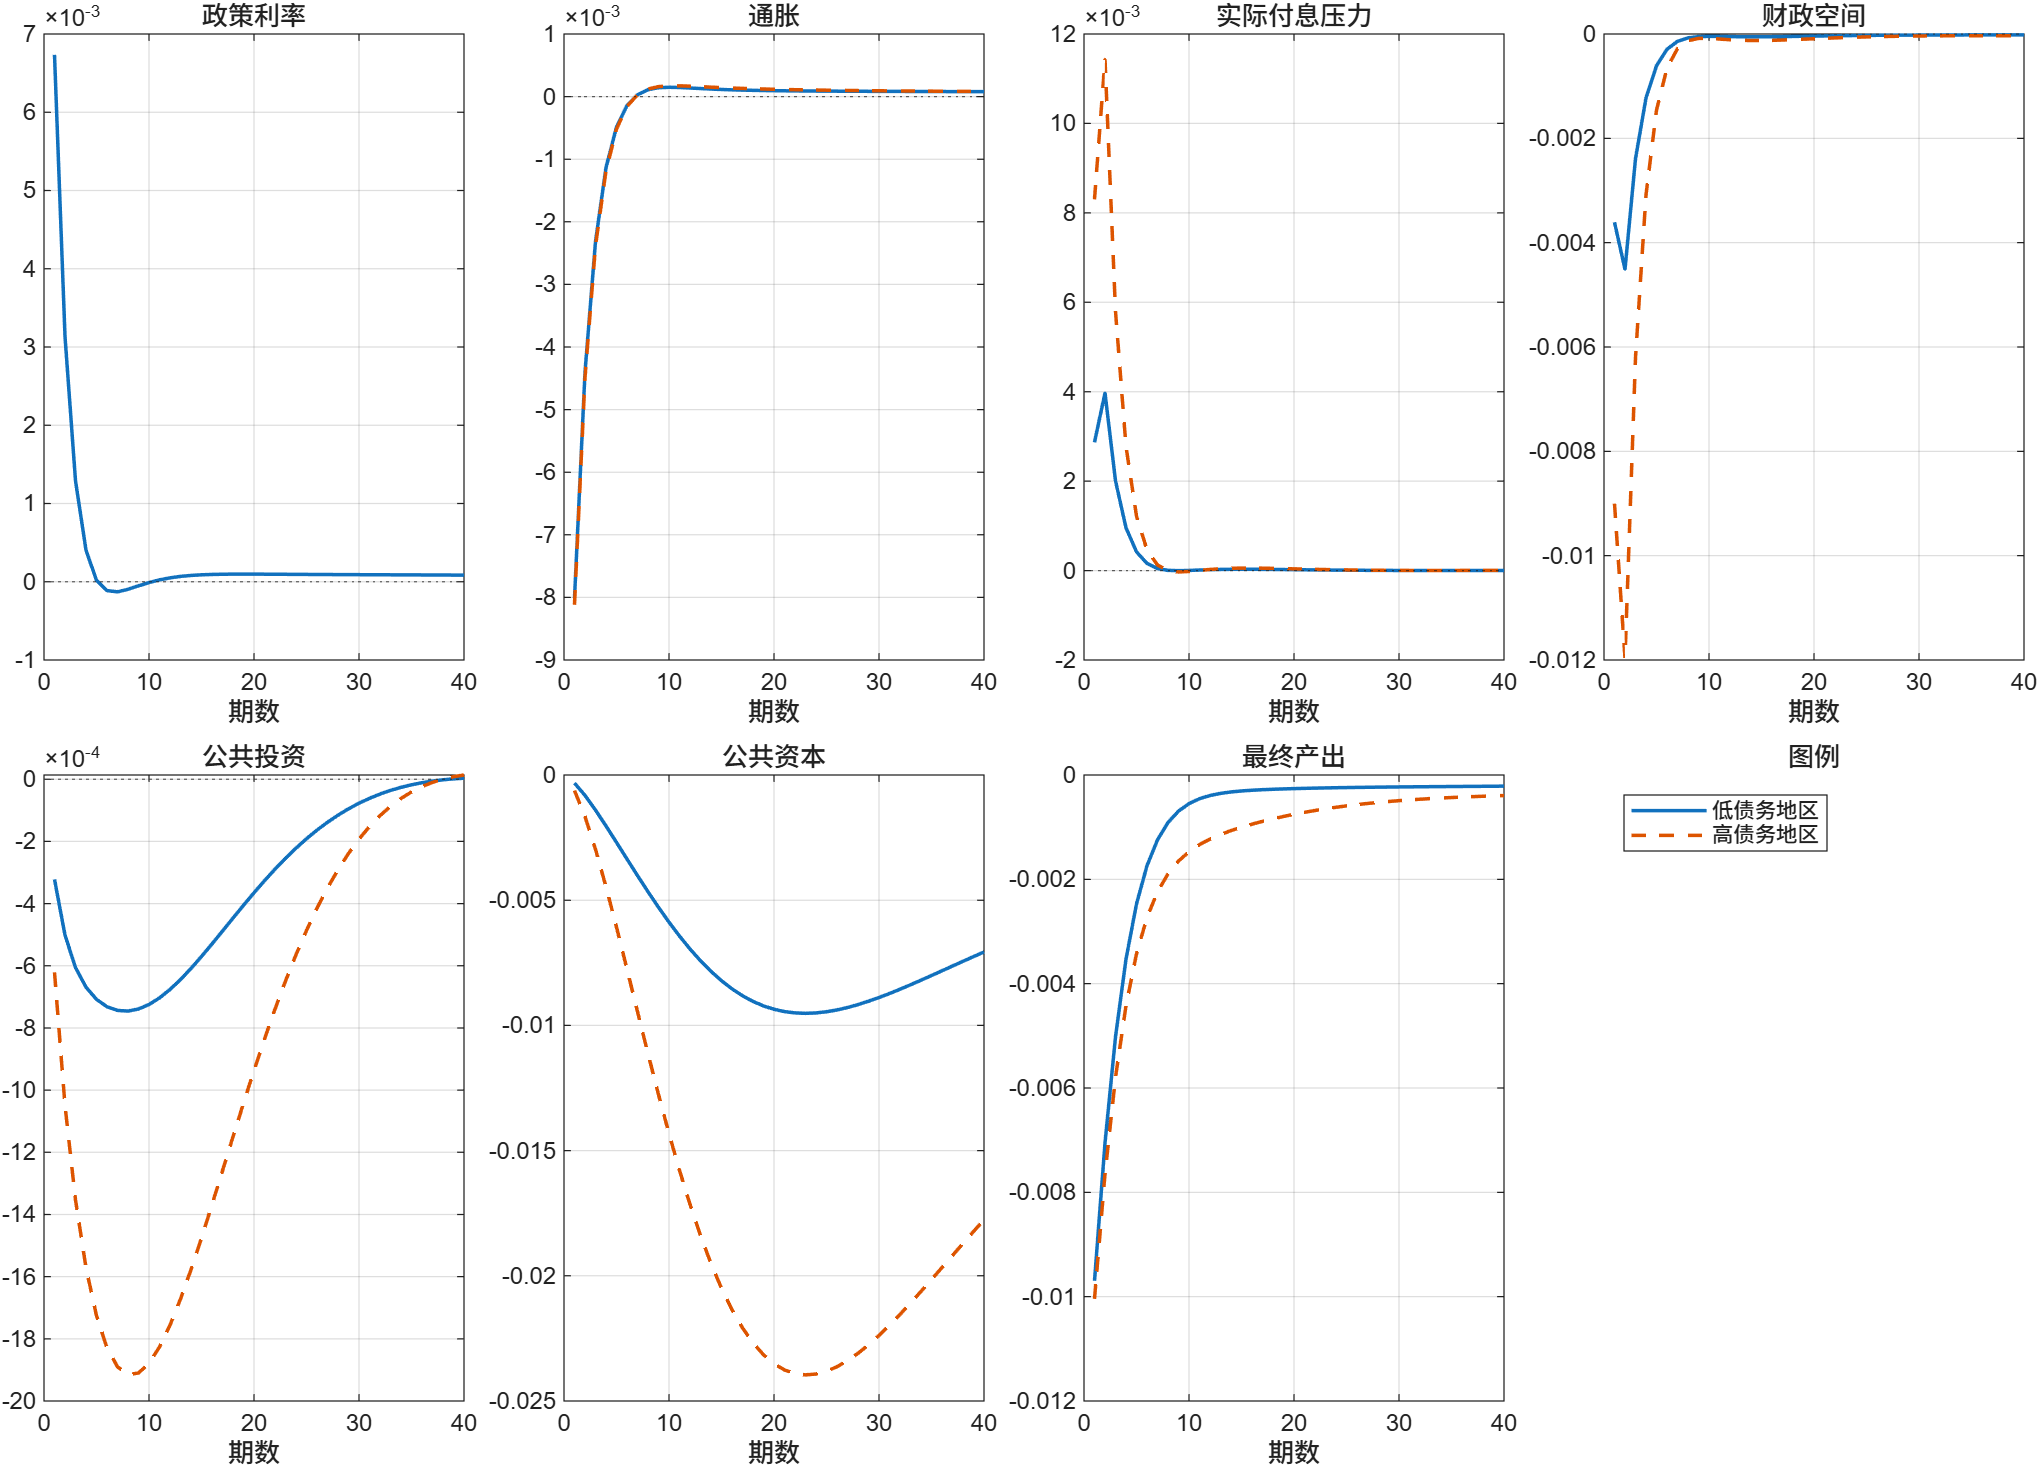
\includegraphics[width=0.90\textwidth]{code/baseline/baseline_irf_comparison.png}
			\caption{基准货币紧缩下的地方债务放大机制脉冲响应对比}
			\label{fig:baseline}
		\end{figure}
		
		在冲击引入当期，由于历史形成的到期名义债务规模属于预定变量，统一宏观紧缩伴随的通胀快速回落瞬间抬升了存量债务的实际偿付负担，导致两地区实际债务服务成本发生剧烈分化。脉冲响应结果显示，在第1期，低债务地区的实际付息压力偏离稳态仅上升0.0029，而高债务地区则大幅飙升0.0083，两地当期付息压力缺口瞬间达到0.0054。由于高债务地区面临更庞大的历史债务基数，同样的物价变动和后续再融资利率上行被进一步成倍放大，导致其可支配财政空间在第1期急剧收缩0.0090，显著深于低债务地区的0.0036。这种初期的财政空间分化直接证明，总量无差异的统一货币冲击在高度异质的地方债务分布环境下，会迅速转化为具有强烈不对称性的区域财政空间冲击。
		
		地方政府可支配财政空间的非对称收缩，通过内生预算约束机制深刻地改变了公共资金的影子价格，进而对生产性基础设施投资产生明显的顺周期“挤出”效应。面对陡增的偿债付息压力，高债务地区地方政府预算约束的影子价格上升更为剧烈，在维持刚性公共消费与债务稳定的跨期权衡下，其新增一单位生产性公共投资的边际机会成本大幅攀升。数值模拟表明，在冲击当期，高债务地区公共投资即表现出更深的下行（下降0.0006，而低债务地区下降0.0003）；至冲击后的第4期，随着再融资成本上升的后效显现，高债务地区公共投资降幅进一步拉大至0.0016，约为低债务地区降幅的两倍以上。由于地方公共投资项目具有多年度建设和跨期累积特征，初期的投资缺口在中长期内不断自我加剧，导致第12期时高债务地区公共资本存量累计下行达0.0172，两地公共资本缺口呈现明显的跨期走宽趋势。
		
		公共资本积累的地区分化，通过生产网络的供给侧外部性渠道进一步向实体经济传导，最终引发区域间产出和居民消费的深刻调整。在中间品生产函数中，公共资本存量的加速萎缩直接压低了私人生产要素的边际生产率，导致高债务地区的实际工资和私人资本租金回报承受额外的长期下行压力。第1期产出面板显示，高债务地区最终品总产出下滑0.0100，深于低债务地区的0.0097；而在脉冲响应中后期，随着公共资本缺口的持续累积，高债务地区的产出复苏斜率表现出更强的滞后性与脆弱性。值得注意的是，这一财政渠道在地区层面上还触发了双居民类型的TANK放大机制：缺乏金融资产平滑手段的Hand-to-Mouth（流动性约束）家庭由于实际工资收入和转移支付的系统性受损，被迫在当期更大幅度地削减消费，从而贡献了极高的即期总需求负乘数，进一步加剧了高债务地区的实体经济恶化。
		
		总体而言，上述基准货币紧缩冲击下的区域非对称响应，完整构成了本文所强调的“地方债务实际付息压力渠道”的量化证据链。这一发现表明，地方政府债务存量在宏观经济运行中并不是一个中性的、可被单纯视为背景变量的稳态参数，而是直接决定总量政策区域传导弹性的关键宏观状态变量。中央银行若仅基于全国加总通胀与产出等指标设定总量政策反应强度，将不可避免地忽视地方财政硬约束在微观层面的非对称传导，进而可能在稳定全国总体波动的同时，反向扩大区域间实体经济的不同步性，这为后文反事实政策分析中引入新型多维调控工具提供了核心的理论和定量基础。

		\subsection{债务率强度弹性与地区规模异质性检验}
		
		为了确认基准模型中非对称传导结果并非源于特定债务率校准的偶然产物，本文首先通过调整区域初始稳态债务水平实施了债务率强度弹性实验。在此项反事实检验中，低债务地区的长期稳态债务/GDP比率被固定为40\%，而高债务地区的稳态债务/GDP比率则依次设定为40\%、80\%、120\%和160\%。其中，两地区债务率同为40\%的情形构成了一个近似的安慰剂实验。数值模拟结果显示，在这一对称债务率的情景下，两地区核心宏观变量的脉冲响应几乎完全重合，其高低差异曲线紧密贴合于零轴，从而有力地排除了偏好、技术、价格刚性或要素网络等其他外生结构非对称对基准结果的干扰，证实了区域传导分化完全是由初始债务存量异质性驱动的。
		
		图\ref{fig:debt_intensity}的四个面板集中展示了在不同债务率强度下，“高债务地区减低债务地区”核心变量的差异脉冲响应轨迹。随着高债务地区初始债务负担的递增，统一货币紧缩所引发的实际付息压力缺口、公共投资缺口、公共资本缺口以及最终产出缺口均呈现出清晰且显著的单调放大关系。当高债务地区的债务率跃升至160\%的高危水平时，第1期由通胀回落和再融资利率上升共同引致的实际付息压力缺口剧烈扩大至0.0100，当期地方生产性公共投资缺口随之加深至-0.00055。这种初期的财政紧缩压力沿供给侧跨期链条持续向下游实体扩散，导致第12期地方公共资本缺口大幅下探至-0.0187，而中长期的最终产出缺口仍维持在-0.0015的深位。上述弹性检验表明，地方政府的债务存量在模型中绝非中性的稳态背景变量，而是决定总量货币政策区域传导弹性的关键宏观状态变量。
		
		\begin{figure}[H]
			\centering
			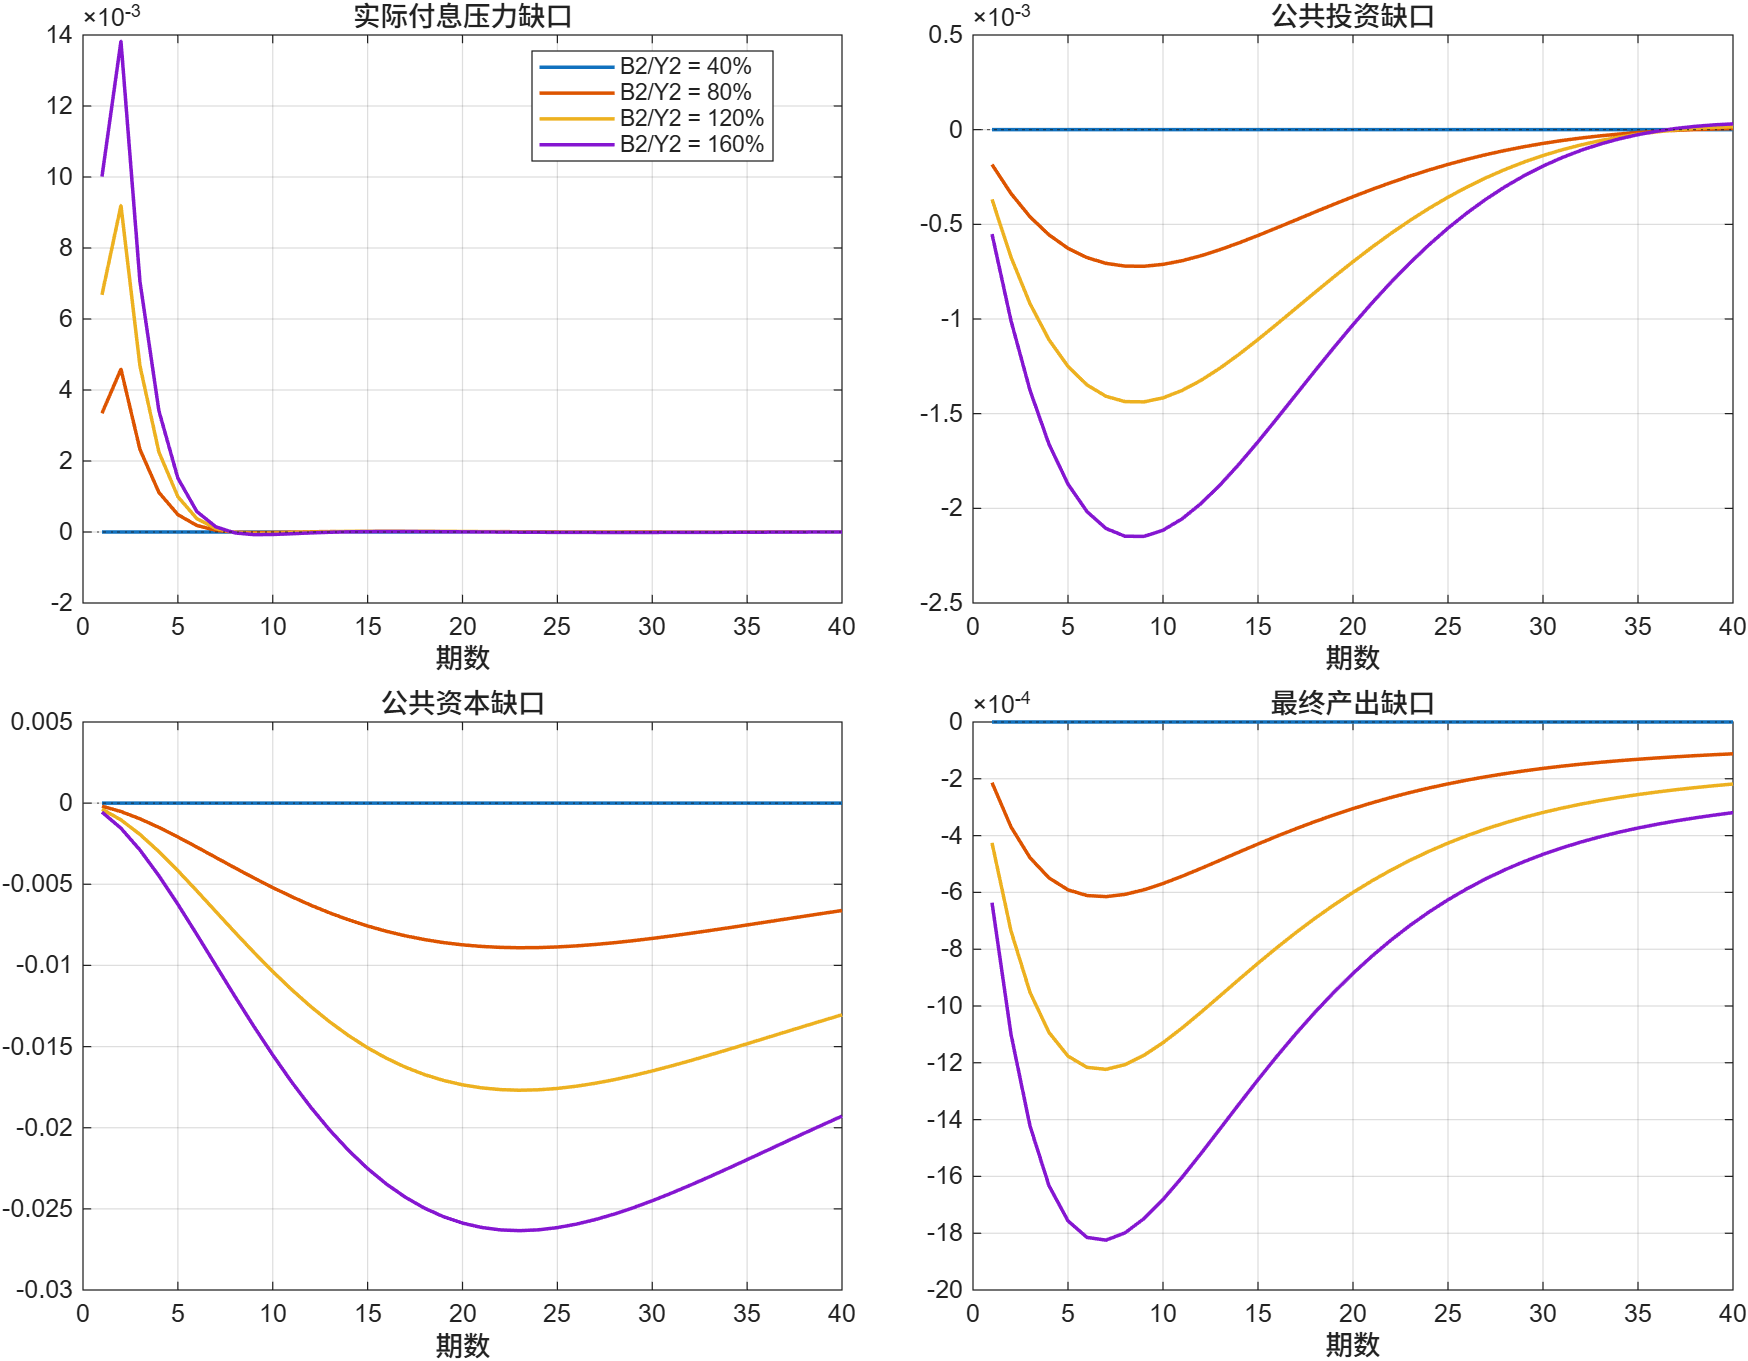
\includegraphics[width=0.90\textwidth]{code/debt_intensity/figure2_debt_intensity_gap_irfs.png}
			\caption{稳态债务率强度提高下的高低债务地区差异响应}
			\label{fig:debt_intensity}
		\end{figure}
		
		在确立了债务强度的单调放大效应后，第二个稳健性检验进一步考察了区域经济规模与发展水平的非均衡设定是否会动摇上述传导机理。在现实宏观经济体中，高债务负担省份往往伴随着欠发达的实体特征，其经济体量占比也与发达低债务地区存在显著差异。为此，本文将发达低债务地区与欠发达高债务地区的稳态产出规模比例 $Y^1/Y^2$ 依次设定为1.0（基准完全对称）、1.5和2.0，并依据产出体量在中央银行的加权 Taylor 利率规则中相应调整各地区的决策权重 $s_1$（分别对应0.500、0.600和0.667）。该项实验旨在检验，当高债务地区在全国总量宏观目标中的代表性下降时，其面临的财政空间紧缩与公共投资挤出机制是否会发生结构性异变。 
		
		表\ref{tab:scale_development_robustness}汇总了高债务欠发达地区在不同规模权重设定下的第1期核心变量响应，而其完整的动态收敛轨迹则由附录图8提供。数值结果表明，随着低债务地区在全国经济体量中权重的持续上升，高债务欠发达地区的核心脉冲响应表现出极高的结构稳健性，各主要变量的峰值偏离几乎保持不变。具体而言，在 $Y^1/Y^2$ 从1.0跃升至2.0的过程中，高债务地区第1期的实际付息压力仅在0.00829至0.00835的极窄区间内微幅浮动，生产性公共投资的即期降幅极其稳定地维持在-0.000620至-0.000623之间，而本地最终产出的当期跌幅则局限在-0.01003至-0.01006的稳定量级。
				
		\begin{table}[H]
			\centering
			\caption{规模与发展异质性稳健性检验：高债务地区第 1 期响应}
			\label{tab:scale_development_robustness}
			\small
			\begin{tabular}{ccccc}
				\toprule
				$Y^1/Y^2$ & Taylor 权重 $s_1$ & $DS_t^2$ & $I_{G,t}^2$ & $Y_t^2$ \\
				\midrule
				1.0 & 0.500 & 0.00829 & -0.000620 & -0.01003 \\
				1.5 & 0.600 & 0.00833 & -0.000622 & -0.01005 \\
				2.0 & 0.667 & 0.00835 & -0.000623 & -0.01006 \\
				\bottomrule
			\end{tabular}
		\end{table}
		
		这一规模异质性检验结果深刻说明，本文所揭示的传导渠道并不是全国 Taylor 规则加权方式变化所导致的机械性或技术性结果。在典型的财政分权与央地税收分成制度环境下，只要地方政府面临着刚性的历史债务付息流与内生的生产性公共投资跨期选择，高昂的债务存量基数就必然会系统性地推高顺周期的财政资金影子价格。无论该地区的绝对经济体量在大国总量决策中占据何种份额，统一货币紧缩引发的“债务实际化”与“再融资成本抬升”都将稳定且持续地通过地方政府资产负债表内生挤出基础设施投资，并在空间层面上强化高债务负担腹地的跨期调整压力。

		\begin{table}[H]
			\centering
			\caption{扩展情景稳健性：高债务地区减低债务地区的差异响应}
			\label{tab:extension_robustness}
			\small
			\resizebox{\textwidth}{!}{%
			\begin{tabular}{lcccccc}
				\toprule
				\textbf{情景} & \multicolumn{2}{c}{\textbf{实际付息压力差异}} & \multicolumn{2}{c}{\textbf{公共投资差异}} & \multicolumn{2}{c}{\textbf{最终产出差异}} \\
				\cmidrule(lr){2-3}\cmidrule(lr){4-5}\cmidrule(lr){6-7}
				& 第 1 期 & 第 12 期 & 第 1 期 & 第 12 期 & 第 1 期 & 第 12 期 \\
				\midrule
				基准 & 0.00543 & 0.000005 & -0.000299 & -0.001080 & -0.000347 & -0.000835 \\
				地方债风险溢价 & 0.00550 & 0.000530 & -0.000554 & -0.001948 & -0.000615 & -0.001409 \\
				中央转移支付缓冲 & 0.00558 & -0.000222 & 0.000734 & 0.003660 & 0.000929 & 0.002917 \\
				强跨地区投入产出联系 & 0.00538 & 0.000015 & -0.000300 & -0.001098 & -0.000342 & -0.001062 \\
				弱跨地区投入产出联系 & 0.00547 & 0.000001 & -0.000299 & -0.001071 & -0.000334 & -0.000697 \\
				\bottomrule
			\end{tabular}}
		\end{table}
		
		\subsection{全国性负向需求冲击下的货币政策稳定反应权衡}
		
		在识别货币紧缩冲击的区域传导后，本文进一步考察全国性负向需求冲击下的政策权衡。需求冲击以阻尼楔子的形式进入 Ricardian 家庭跨期 Euler 方程 \eqref{a2}，其外生过程由式 \eqref{a41D} 给出，并设定持续性 $\rho_D=0.80$。实验将 Taylor 规则中的通胀反应系数设为 $\phi_\pi \in \{1.1, 1.5, 2.0, 2.5, 3.0\}$，用于评估更强的通胀稳定反应是否一定能够改善整体宏观表现。图 \ref{fig:stability_sync} 将各情形的动态路径压缩为“总体波动--区域不同步”二维空间。
		
		\begin{figure}[H]
			\centering
			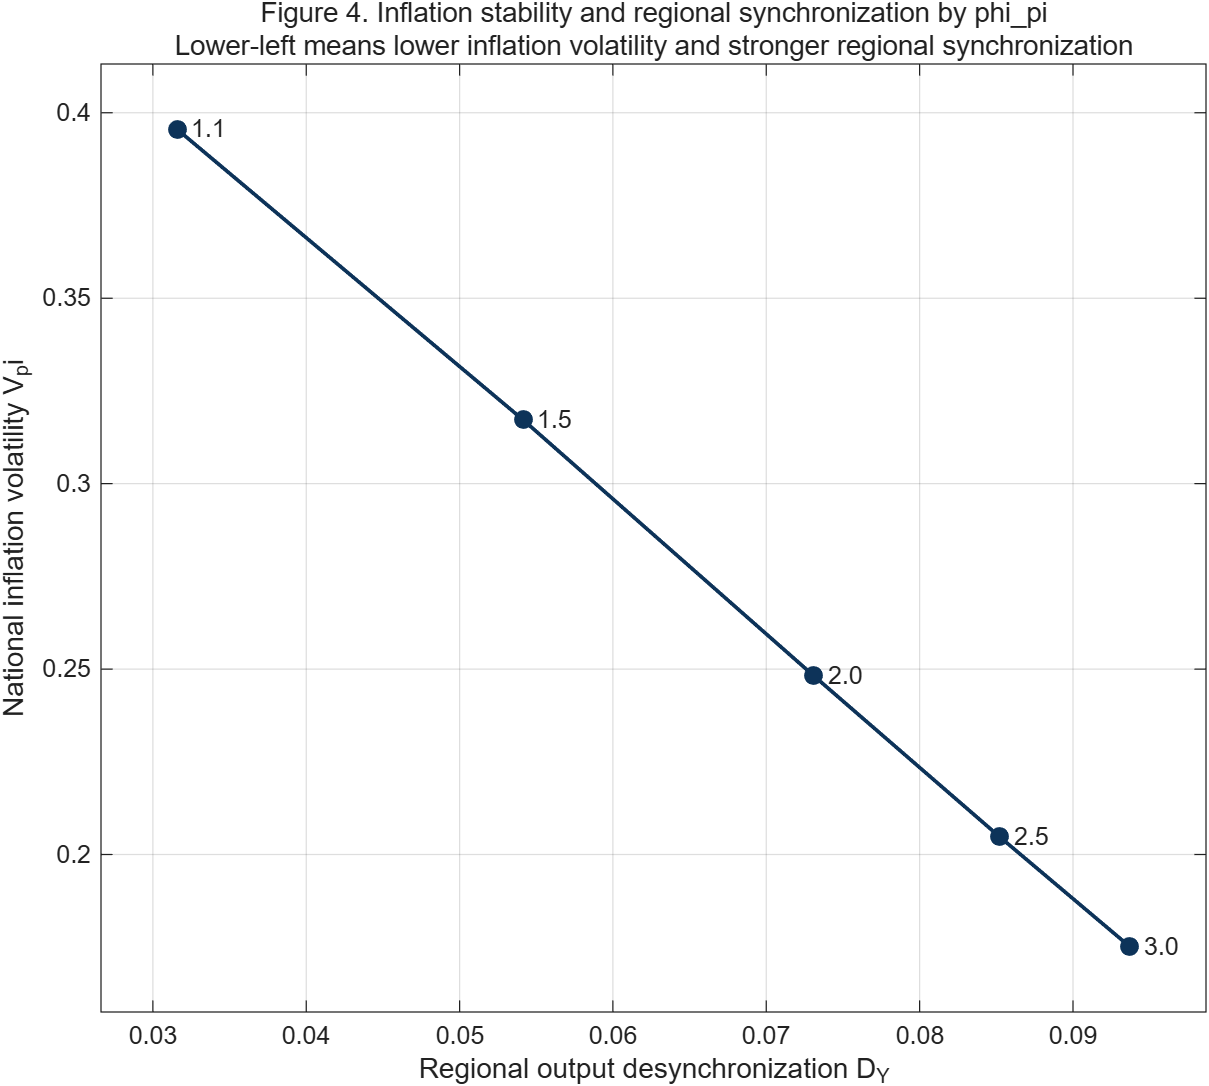
\includegraphics[width=0.80\textwidth]{code/demand_monetary/figure4_negative_demand_stability_sync_map.png}
			\caption{负向需求冲击下货币政策通胀反应系数的稳定性--同步性两难权衡}
			\label{fig:stability_sync}
		\end{figure}
		
		图 \ref{fig:stability_sync} 的横轴为地区间产出不同步程度，纵轴为全国通胀波动范数，因而越接近左下方代表同时实现更低总量波动和更高区域同步性。图中点旁数字表示 Taylor 规则中的通胀反应系数 $\phi_\pi$。随着 $\phi_\pi$ 从 1.1 提高至 3.0，全国通胀波动范数由 $0.396$ 降至 $0.175$，全国总产出波动范数由 $0.511$ 降至 $0.216$。这说明更强的通胀稳定反应能够有效压低全国层面的价格和产出波动。
		
		然而，总量稳定的改善并未自动转化为区域同步性的改善。地区间产出不同步程度 $\mathcal D_Y$ 从 $0.0316$ 单调上升至 $0.0937$。其原因在于，统一利率规则只能针对全国加总变量作出反应，无法直接补偿地区财政空间的异质性约束；当高债务地区公共投资对实际付息压力更敏感时，更强的总量稳定政策会改变实际利率、税基、公共投资和公共资本的相对调整时序，从而扩大地区产出路径差异。因此，在存在地方债务异质性的经济中，中央银行若只依据全国通胀和全国产出缺口设定反应强度，可能面对“总量更稳定、区域更不同步”的政策两难。
		
		\subsection{两类反事实政策工具的治理成效评估与比较}
		
		上述两难说明，单一货币政策难以同时完成全国稳定和区域协调目标。为此，本文在基准模型之外设计两类反事实政策工具，以识别财政制度安排对债务放大机制的缓冲或约束作用。第一类是严格债务余额限额，其核心目标是压低地方债务风险暴露；第二类是反周期中央转移支付稳定器，其核心目标是在冲击期补充高债务地区财政空间。二者并非同一政策目标下的简单优劣比较，而是分别代表“风险约束”和“稳定缓冲”两种治理逻辑。
		
		为与基准模型保持清晰区分，以下规则仅在反事实实验中启用。债务余额限额规则不再采用平滑惩罚函数，也不再直接约束当期 $B/Y$ 比例，而是设定为高债务地区地方债务余额的硬性上限：
		\begin{equation}
			B_t^2\leq \bar B_{\max}^2,\qquad
			\mathcal U_t^2\equiv \frac{B_t^2}{\bar B_{\max}^2}\leq 1.
			\label{eq:strict_debt_cap}
		\end{equation}
		这一设定更接近中国地方政府债务余额限额管理：法定约束对象是经批准的债务余额，而非随当期产出波动而机械变化的债务率分母。本文将高债务地区的严格余额上限校准为 $\bar B_{\max}^2=1.00$，即稳态债务余额本身就是法定上限，代表高债务地区在冲击期不得继续净新增债务余额；低债务地区的参照上限设为 $0.37$，使其稳态限额使用率低于高债务地区。技术上，本文使用 OccBin 方法求解偶尔绑定约束：当放松 regime 下 $B_t^2-\bar B_{\max}^2>0$ 时，模型切换到绑定 regime，并以 $B_t^2=\bar B_{\max}^2$ 替代债务限额松弛条件；当债务限额影子价格转负时，模型返回放松 regime。该设定刻画硬性债务余额限额对地方再融资空间的直接约束，而不是在地方政府目标函数中额外加入连续惩罚项。需要强调的是，图中水平边界对应的是限额使用率 $\mathcal U_t^2=B_t^2/\bar B_{\max}^2$，而 $B_t^2/Y_t^2$ 仍会因为 $Y_t^2$ 的变化而波动，因此不应要求债务率本身机械水平。
		
		中央转移支付稳定器则保持地方政府预算约束 \eqref{eq:gov_budget} 的结构不变，仅将 $Z_t^j$ 从稳态财政闭合项拓展为对地方财政压力作出反周期反应的政策工具：
		\begin{equation}
			\log\left(\frac{Z_t^j}{\bar Z^j}\right)
			=\rho_Z\log\left(\frac{Z_{t-1}^j}{\bar Z^j}\right)
			+\phi_{Z,DS}\left(\frac{DS_t^j}{\bar{DS}^j}-1\right)
			+\phi_{Z,B}\left(\frac{B_{t-1}^j/Y_{t-1}^j}{\bar B^j/\bar Y^j}-1\right).
			\label{eq:Z_rule_ext}
		\end{equation}
		该规则不再引入独立的中央转移支付随机冲击，而是使转移支付随地方实际付息压力和债务率偏离内生调整。本文设定 $\phi_{Z,DS}=0.015$、$\phi_{Z,B}=0.005$，即中央财政对短期付息压力的反应强于对债务存量偏离的反应，但总体强度保持在部分缓冲而非完全对冲的范围内。这一设定体现了中央财政在局部流动性压力上升时提供定向缓冲、但不完全兜底地方债务存量风险的制度含义。由于 $Z_t^j$ 作为地方政府预算收入项进入 \eqref{eq:gov_budget}，其稳定作用通过降低财政资金影子价格 $\Lambda_{G,t}^j$ 间接支撑条件最优公共投资。

		为避免将中央转移支付误解为无成本政策，本文同时定义中央财政的当期净转移成本：
		\begin{equation}
			\Delta Z_t^{C}
			\equiv
			\sum_{j=1}^{2}s_j\left(Z_t^j-\bar Z^j\right).
			\label{eq:central_transfer_cost}
		\end{equation}
		若将中央政府预算约束显式展开，则该成本需要由当期中央税收、中央债务或未来一次性税收融资。本文的反事实实验暂不把未来中央融资税负反馈到家庭福利和地方需求中，因此图 \ref{fig:central_transfer} 报告的是中央转移支付对地方财政空间的总缓冲效应，而不是扣除中央财政融资成本后的净社会福利效应。若采用严格收入中性的实施方式，稳定器对福利的正向作用会被未来税负部分抵消。
		
		债务余额限额实验将高债务地区硬性上限设为 $B_t^2\leq 1.00$。在标准货币紧缩冲击下，基准模型中高债务地区债务余额限额使用率峰值为 $1.0257$，意味着若没有硬性余额约束，债务余额会超过法定上限约 $2.57\%$；严格限额规则将该指标压在 $1.0000$。图 \ref{fig:debt_limit_high_debt} 聚焦高债务地区在基准模型与严格余额限额规则下的 IRF；图 \ref{fig:debt_limit_diff} 进一步报告“严格余额限额规则减基准模型”的差异响应。两地区完整核心变量 IRF 列于附录图 \ref{fig:app_debt_limit_regions}。
		
		\begin{figure}[H]
			\centering
			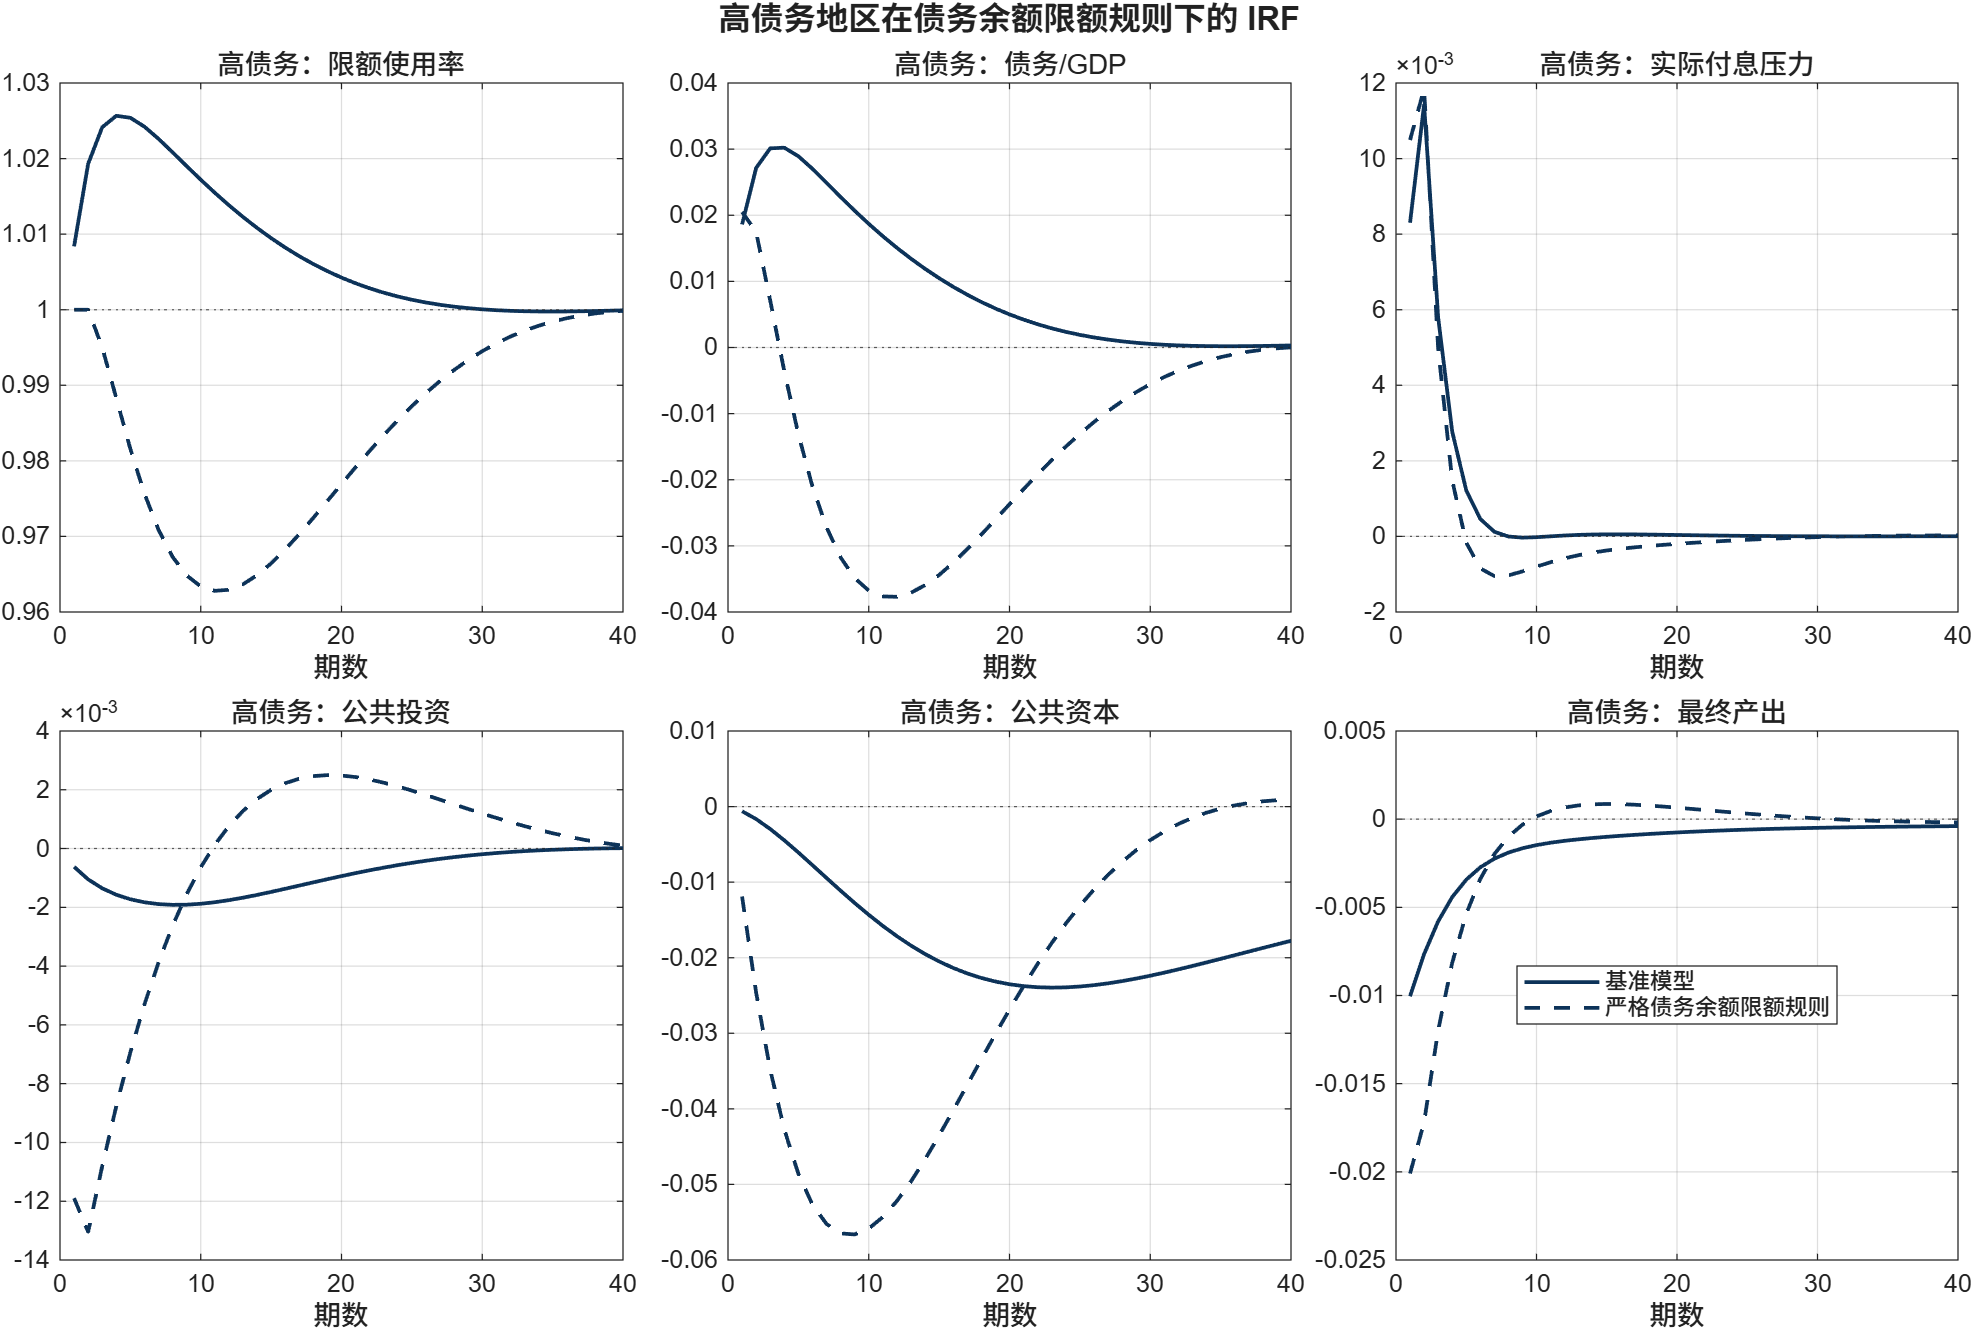
\includegraphics[width=0.90\textwidth]{code/policy_counterfactual/figure5_debt_limit_high_debt_irfs.png}
			\caption{反事实政策实验：高债务地区在严格债务余额限额规则下的 IRF}
			\label{fig:debt_limit_high_debt}
		\end{figure}
		
		图 \ref{fig:debt_limit_high_debt} 显示，硬性余额限额使高债务地区限额使用率在绑定期内被压在 $\mathcal U_t^2=1$ 的上限处，随后随着公共投资压缩和预算调整转入上限以下。与基准路径相比，严格限额明显降低了债务余额风险暴露，并使债务/GDP 峰值由 $1.0302$ 降至 $1.0205$。但是，债务约束并非无成本稳定器。绑定期内，地方政府不能完全依靠新增债务吸收付息压力，公共投资需要承担更大的预算调整，最终产出也出现额外损失。
		
		\begin{figure}[H]
			\centering
			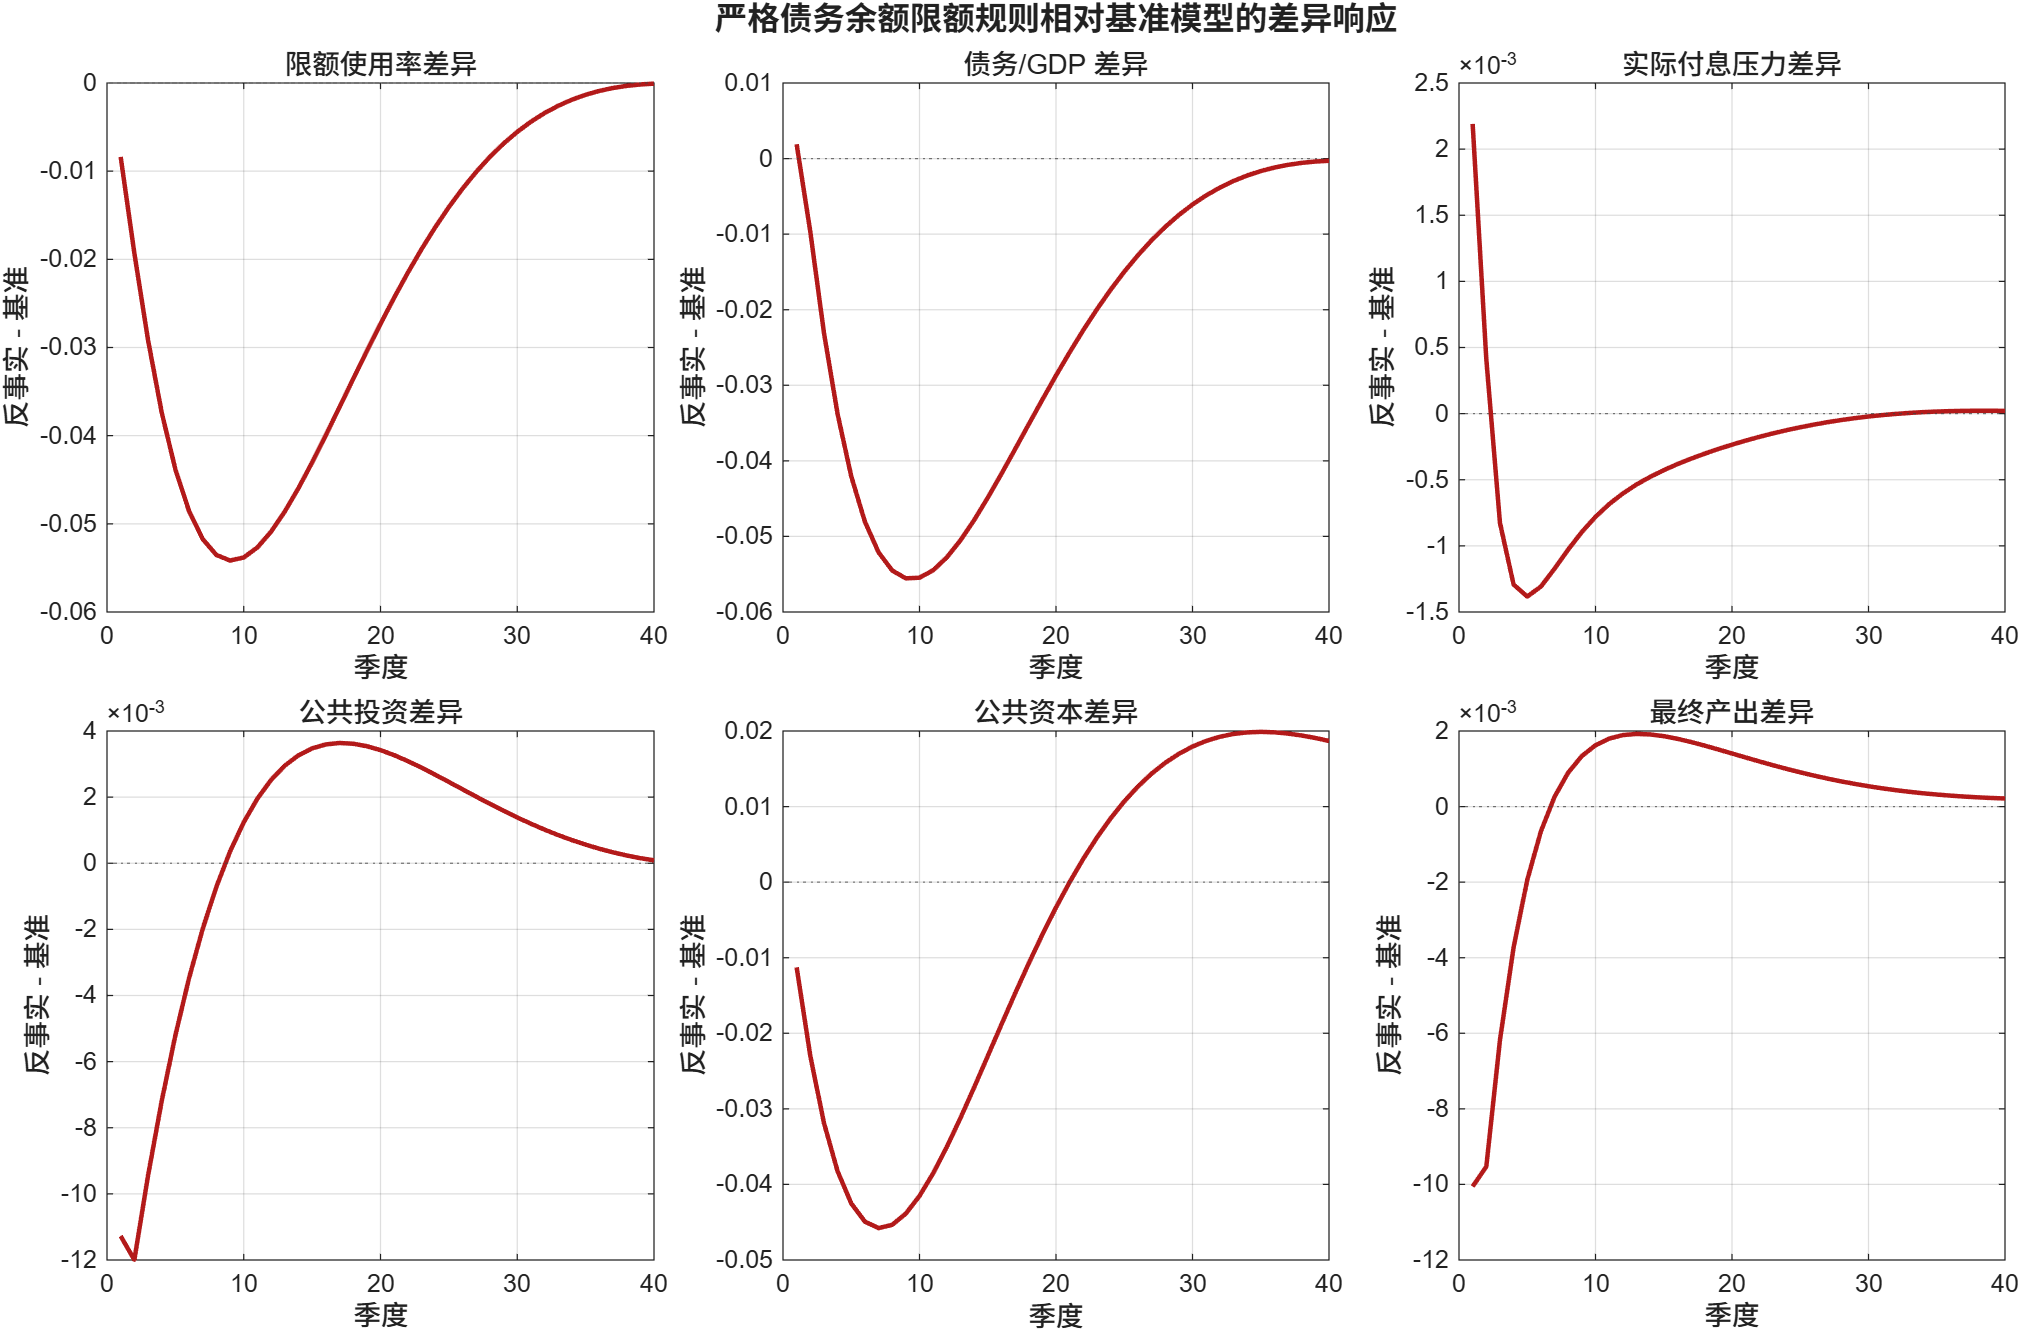
\includegraphics[width=0.90\textwidth]{code/policy_counterfactual/figure5_debt_limit_diff_irfs.png}
			\caption{反事实政策实验：严格债务余额限额规则相对基准模型的差异响应}
			\label{fig:debt_limit_diff}
		\end{figure}
		
		图 \ref{fig:debt_limit_diff} 将严格余额限额规则的增量效应单独画出，零线表示基准路径，红线低于零表示严格限额规则下该变量低于基准情形。数值结果表明，冲击后高债务地区限额使用率峰值由基准情形的 $1.0257$ 降至 $1.0000$，超限压力降至零；债务/GDP 峰值由 $1.0302$ 降至 $1.0205$。与此同时，公共投资谷值由 $-0.0019$ 加深至 $-0.0130$，最终产出谷值由 $-0.0100$ 加深至 $-0.0201$。因此，硬性债务余额上限能够直接压低债务风险暴露，但其治理逻辑具有明显顺周期调整成本：当地方政府不能通过新增债务平滑冲击时，公共投资和产出需要承担更大的短期调整。
		
		与债务余额限额规则不同，反周期中央转移支付稳定器直接作用于地方预算收入端。本文激活式 \eqref{eq:Z_rule_ext} 描述的定向转移规则，并比较其相对于无稳定器情形的缓冲效果。图 \ref{fig:central_transfer} 报告高债务地区核心变量的响应。
		
		\begin{figure}[H]
			\centering
			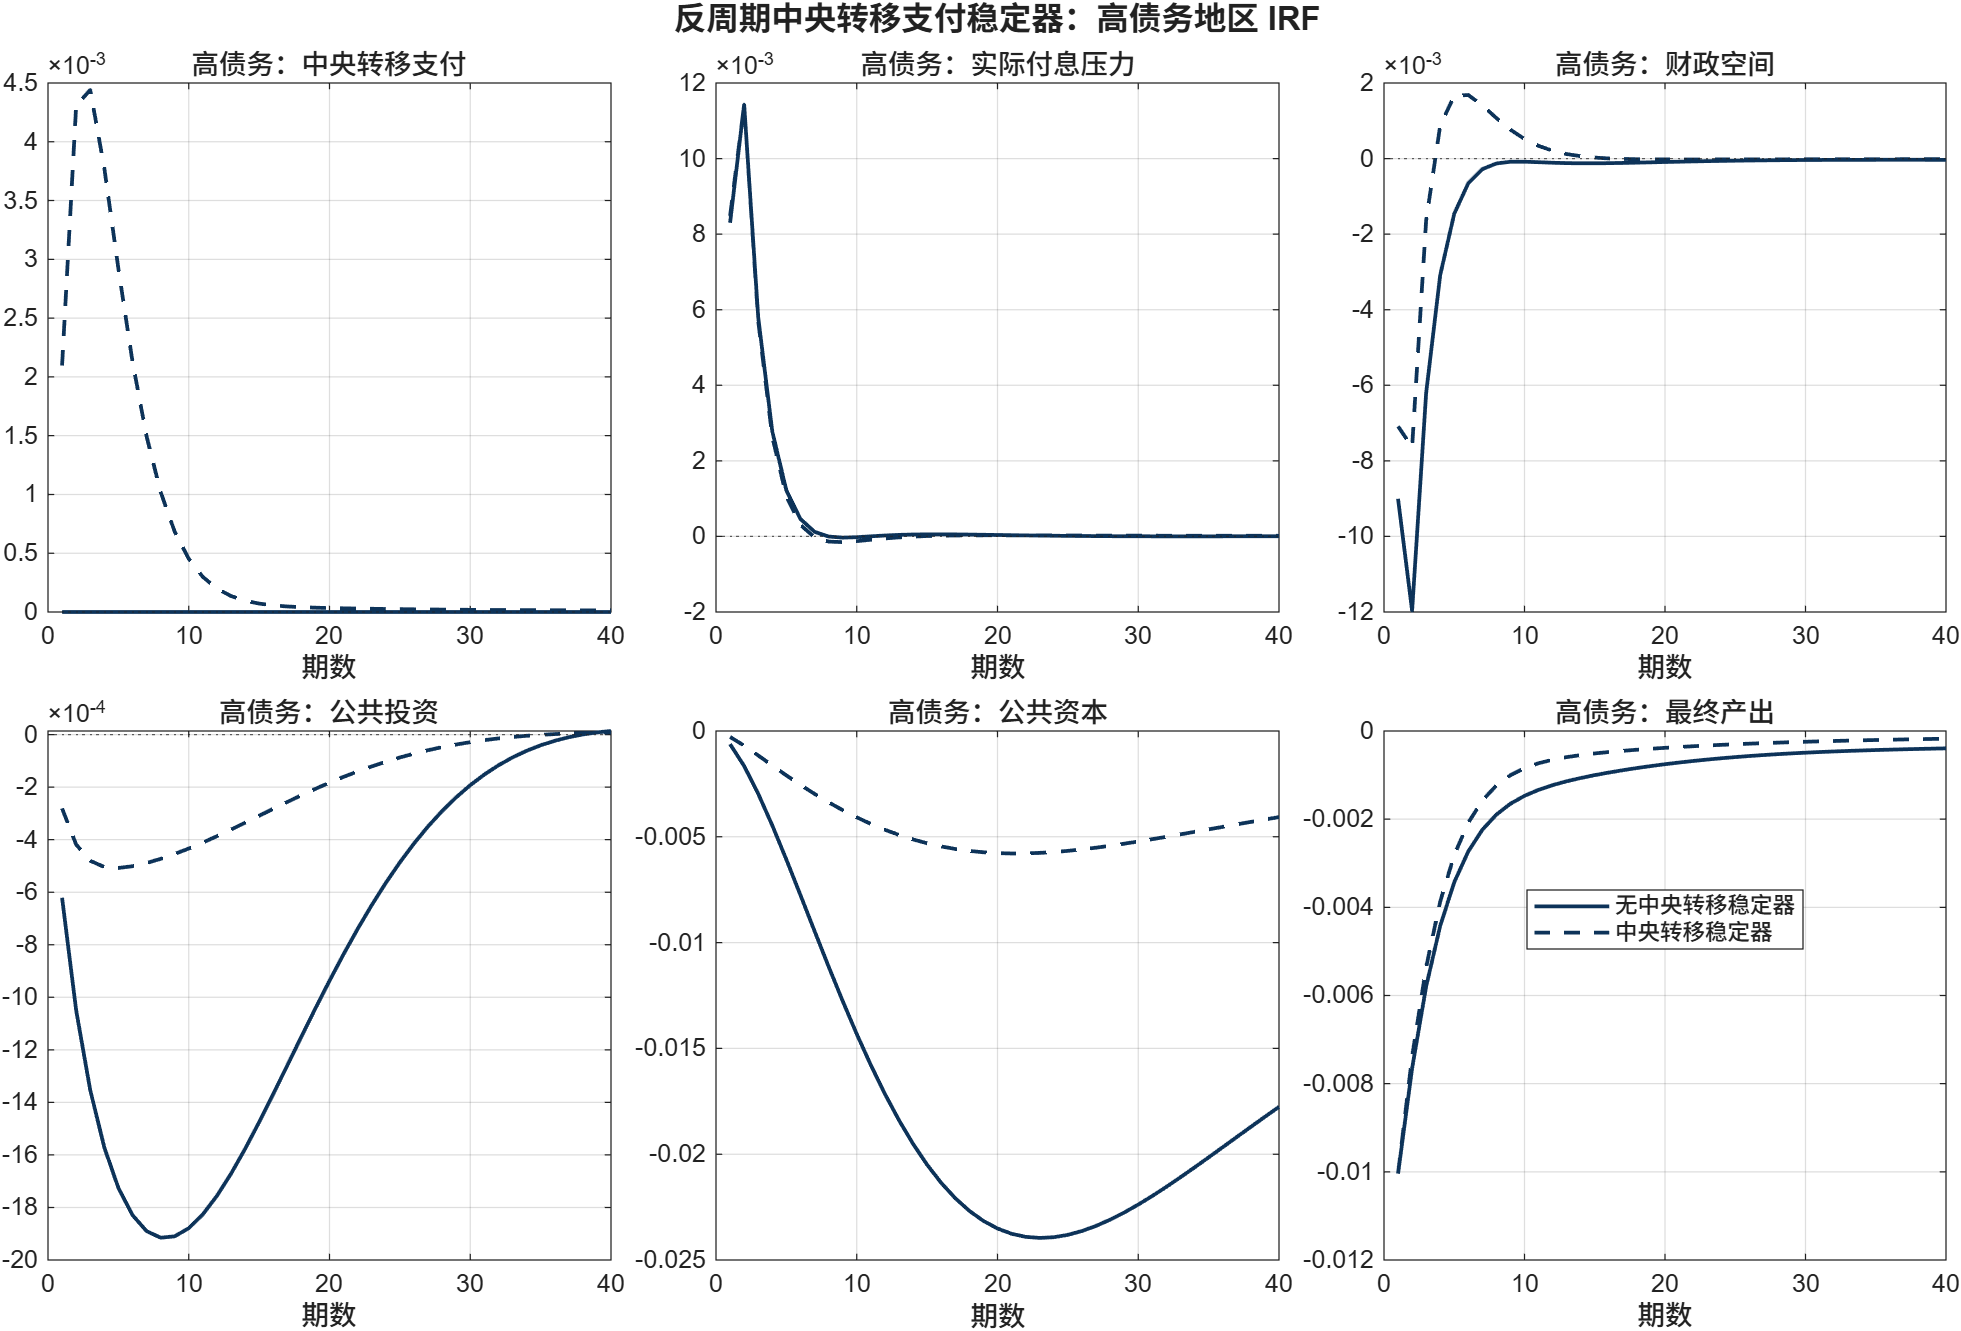
\includegraphics[width=0.90\textwidth]{code/policy_counterfactual/figure6_central_transfer_high_debt_irfs.png}
			\caption{反事实政策实验：反周期中央转移支付稳定器对高债务地区的平抑缓冲效应}
			\label{fig:central_transfer}
		\end{figure}
		
		图 \ref{fig:central_transfer} 的关键在于比较“无中央转移稳定器”和“中央转移稳定器”两条路径。中央转移支付面板显示，稳定器在冲击初期自动增加拨付；财政空间面板显示，该拨付缓解了高债务地区预算收缩；公共投资和公共资本面板则展示这一缓冲如何继续传导到实体供给侧。数值上，高债务地区公共投资 $I_{G,t}^2$ 的谷值由基准情形下的 $-0.0019$ 改善至 $-0.0005$，公共资本 $K_{G,t}^2$ 的谷值由 $-0.0240$ 改善至 $-0.0058$。同时，高低债务地区产出差异峰值由 $0.0010$ 降至 $0.00082$。这说明，中央转移支付稳定器的主要作用不是改变公共投资响应方向，而是在保持负向调整方向的同时削弱其幅度，从而缓和“付息压力--财政空间收缩--公共投资下降”的传导链条；但这一结论应与式 \eqref{eq:central_transfer_cost} 所提示的中央财政成本一并理解。

		表 \ref{tab:central_transfer_cost} 进一步把这一成本显式量化。中央转移稳定器下，高债务地区转移支付偏离的峰值为 $0.0044$，全国加权净转移成本 $\Delta Z_t^C$ 的峰值为 $0.0043$；按 12 期和 40 期累计分别为 $0.0224$ 与 $0.0225$。该结果意味着，中央转移支付稳定器在模型中确实能缓冲地方财政空间，但其政策评价必须同时考虑中央财政融资、跨地区再分配和兜底预期。

		\begin{table}[H]
			\centering
			\caption{中央转移支付稳定器的缓冲效应与财政成本}
			\label{tab:central_transfer_cost}
			\small
			\begin{tabular}{lcc}
				\toprule
				\textbf{指标} & \textbf{无中央转移稳定器} & \textbf{中央转移稳定器} \\
				\midrule
				高债务地区转移支付峰值 $Z_t^2-\bar Z^2$ & 0.0000 & 0.0044 \\
				全国加权净转移成本峰值 $\max_t \Delta Z_t^C$ & 0.0000 & 0.0043 \\
				前 12 期累计净转移成本 $\sum_{t=1}^{12}\Delta Z_t^C$ & 0.0000 & 0.0224 \\
				前 40 期累计净转移成本 $\sum_{t=1}^{40}\Delta Z_t^C$ & 0.0000 & 0.0225 \\
				高债务地区公共投资谷值 $\min_t I_{G,t}^2$ & -0.0019 & -0.0005 \\
				地区产出差异峰值 $\max_t |Y_t^2-Y_t^1|$ & 0.0010 & 0.00082 \\
				\bottomrule
			\end{tabular}
		\end{table}
		
		\subsection{总体波动与多维异质性居民福利的综合定量评估}
		
		最后，本文对不同货币政策通胀反应强度进行规范性评价。表 \ref{tab:policy_eval} 在负向需求冲击下同时报告全国总体波动、地区不同步程度、区域实际付息压力差异以及基于两地区、两类家庭计算得到的有限期条件消费等价福利变化（CEV）。其中，$\phi_\pi=1.5$ 作为经典 Taylor 规则基准，其他情形的福利变化均相对于该基准计算。

		具体而言，给定 Dynare 一阶 IRF 生成的消费和劳动水平路径，家庭类型 $h\in\{R,H\}$、地区 $j$ 的有限期条件福利定义为
		\begin{equation}
			W_h^j
			=
			\sum_{t=0}^{T-1}\beta^t
			\left[
			\frac{(C_{h,t}^j)^{1-\sigma}}{1-\sigma}
			-\chi_N\frac{(N_{h,t}^j)^{1+\varphi}}{1+\varphi}
			\right],
			\qquad T=40.
			\label{eq:welfare_def}
		\end{equation}
		地区和全国福利分别按照人口权重 $\lambda_j$ 与地区产出权重 $s_j$ 加总。对任一备择政策规则 $r$，其相对于基准规则 $0$ 的消费等价变化 $\xi_r$ 由下式隐含定义：
		\begin{equation}
			\sum_{j,h}\omega_h^j
			\sum_{t=0}^{T-1}\beta^t
			u\left((1+\xi_r)C_{h,t}^{j,0},N_{h,t}^{j,0}\right)
			=
			\sum_{j,h}\omega_h^j
			\sum_{t=0}^{T-1}\beta^t
			u\left(C_{h,t}^{j,r},N_{h,t}^{j,r}\right),
			\label{eq:cev_def}
		\end{equation}
		其中 $\omega_R^j=s_j(1-\lambda_j)$、$\omega_H^j=s_j\lambda_j$。因此，$\xi_r>0$ 表示若要使基准规则达到备择规则的有限期条件福利，需要把基准路径上的消费等比例提高 $\xi_r$。由于本文使用一阶近似 IRF 和有限期路径，表 \ref{tab:policy_eval} 的福利排序应理解为条件福利比较，而非完整二阶近似下的无条件福利排序。该福利度量也没有内生计入中央转移支付政策的未来融资税负，因此更适合作为不同货币政策反应强度下居民类型暴露差异的诊断指标，而不是最终政策福利判据。
		
		\begin{table}[H]
			\centering
			\caption{负向需求冲击下不同通胀反应系数的波动与多维居民福利评估表}
			\label{tab:policy_eval}
			\small
			\resizebox{\textwidth}{!}{%
				\begin{tabular}{lccccc}
					\toprule
					\textbf{核心评估指标} & $\bm{\phi_\pi=1.1}$ & $\bm{\phi_\pi=1.5}$ & $\bm{\phi_\pi=2.0}$ & $\bm{\phi_\pi=2.5}$ & $\bm{\phi_\pi=3.0}$ \\
					\midrule
					全国总体通胀波动范数 $\mathcal V_\pi$ & 0.396 & 0.317 & 0.248 & 0.205 & 0.175 \\
					全国总体产出波动范数 $\mathcal V_Y$ & 0.511 & 0.398 & 0.308 & 0.253 & 0.216 \\
					地区间产出不同步程度 $\mathcal D_Y$ & 0.0316 & 0.0541 & 0.0731 & 0.0852 & 0.0937 \\
					地区间通胀不同步程度 $\mathcal D_\pi$ & 0.0013 & 0.0024 & 0.0034 & 0.0041 & 0.0045 \\
					区域间实际付息压力差异 $\mathcal D_{DS}$ & 0.255 & 0.225 & 0.207 & 0.202 & 0.201 \\
					\midrule
					全国总体福利 CEV（\%） & 0.0030 & 0.0000 & -0.0030 & -0.0050 & -0.0064 \\
					低债务地区总体福利 CEV（\%） & 0.0022 & 0.0000 & -0.0024 & -0.0039 & -0.0050 \\
					高债务地区总体福利 CEV（\%） & 0.0038 & 0.0000 & -0.0037 & -0.0061 & -0.0078 \\
					全社会 Ricardian 家庭福利 CEV（\%） & 0.0124 & 0.0000 & -0.0111 & -0.0183 & -0.0232 \\
					全社会 Hand-to-Mouth 家庭福利 CEV（\%） & -0.0189 & 0.0000 & 0.0159 & 0.0259 & 0.0328 \\
					\bottomrule
			\end{tabular}}
			\begin{flushleft}
				\footnotesize 注：福利指标为以 $\phi_\pi=1.5$ 的经典规则为基准、根据 40 期一阶 IRF 路径所解得的有限期条件消费等价变化。若 $\text{CEV}>0$ 代表该政策相比基准增进了该主体的条件福利。波动与不同步指标均基于 Dynare 一阶 IRF 数值扩大 100 倍后计算 L2 范数得到。本表比较货币政策反应强度，不扣除前文中央转移支付反事实中的未来中央融资税负，也不包含二阶风险修正项。
			\end{flushleft}
		\end{table}
		
		表 \ref{tab:policy_eval} 表明，货币政策强度的条件福利排序并不等同于总量波动排序。高强度通胀稳定反应（$\phi_\pi=3.0$）使全国通胀和产出波动最低，但相对于基准规则带来全社会总体 CEV 损失（$-0.0064\%$），且高债务地区 CEV 损失（$-0.0078\%$）深于低债务地区（$-0.0050\%$）。相反，较弱通胀反应（$\phi_\pi=1.1$）在本校准下提高了总体 CEV，但代价是更高的全国通胀和产出波动。因此，表 \ref{tab:policy_eval} 的含义不是给出无条件最优 Taylor 系数，而是提示政策评价不能只依据单一总量波动指标，还应同时报告宏观稳定、区域同步和异质性居民福利暴露。
		
		居民类型之间的福利分化同样值得重视。相较于基准规则，$\phi_\pi=3.0$ 使全社会 Ricardian 家庭的 CEV 下降 $0.0232\%$，但使 Hand-to-Mouth 家庭的 CEV 上升 $0.0328\%$。这一结果反映出两类家庭在模型中的风险暴露不同：Ricardian 家庭能够跨期平滑消费并持有资本与金融资产，其福利更受跨期价格、利率和资产回报路径影响；Hand-to-Mouth 家庭缺乏储蓄缓冲，其福利更依赖当期劳动收入、转移支付和价格稳定环境。由此可见，在存在地方债务财政空间约束的经济中，代表性居民框架会掩盖地区之间和家庭类型之间的福利再分配效应。
		
		综合来看，本节的定量结果形成了相互衔接的证据链：统一货币紧缩通过高债务地区更高的实际付息压力压缩财政空间，进而抑制公共投资和公共资本积累；该机制随债务率提高而增强，并对地区规模设定保持稳健；在全国性需求收缩下，更强的通胀稳定反应虽然降低总量波动，却可能扩大地区产出不同步；严格债务余额限额有助于约束风险暴露，但短期内可能强化公共投资收缩；中央转移支付稳定器则能够更直接地缓冲高债务地区的财政空间压力。这些结果为下一节的政策启示提供了定量基础。

		\subsection{数值实现与可复现性说明}

		本文所有数值实验均基于 Dynare 一阶近似求解，并使用 \texttt{stoch\_simul}（\texttt{order=1, irf=40}）生成 40 期脉冲响应。实现文件和输出口径如下：
		\begin{itemize}[leftmargin=2em,itemsep=0.1em]
			\item 基准模型文件：\path{code/baseline/TANK_two_region_baseline.mod}。
			\item 实验脚本目录：\path{code/debt_intensity/}、\path{code/scale_development/}、\path{code/demand_monetary/} 与 \path{code/policy_counterfactual/}。
			\item 数值输出文件：各实验目录下的 \path{status.csv}、\path{summary.csv} 与 \path{irf_series.csv}。
		\end{itemize}
		正文表格中的核心数值直接来自这些汇总文件，图形则由相同 IRF 序列绘制。

		本文修订稿的数值结果在 Windows 环境下使用 MATLAB R2026a 与 Dynare 7.0 生成。复现顺序为：先运行 \path{code/baseline/run_baseline.m} 生成基准结果，再分别运行各实验目录下以 \path{run_*.m} 命名的脚本生成债务率强度、地区规模、需求冲击、政策反事实和扩展情景输出。各目录中 \path{*_status.csv} 用于记录实验是否成功收敛，\path{*_summary.csv} 或 \path{*_key_diffs.csv} 用于生成正文表格，\path{*_irf_series.csv} 用于绘制正文和附录图形。正文新增表格均由这些 CSV 输出直接整理得到。

		由于本文报告的是确定性脉冲响应而非随机模拟样本，图表生成不依赖随机种子。所有 IRF 默认为变量相对于确定性稳态的水平偏离；在负向需求冲击政策评价表中，波动和不同步指标使用扩大 100 倍后的序列计算 L2 范数。本文暂未使用二阶近似计算无条件福利，因此福利结果不应与包含风险修正项的二阶福利分析混同。
		
		\section{研究结论与政策启示}
		
		本文围绕统一货币政策在地方债务异质性背景下的区域传导问题，构建了一个两地区、双居民类型的 TANK--DSGE 模型。模型将央地税收分成、地方政府名义债务、内生公共投资、跨地区投入网络以及 Ricardian 与 Hand-to-Mouth 居民并入同一分析框架，旨在说明同一货币政策冲击为何会在不同债务负担地区产生不同的财政调整和实体经济后果。与仅从居民异质性或总需求渠道解释货币政策传导的框架相比，本文的核心结论是：地方政府资产负债表本身可以成为统一货币政策区域非对称效应的重要放大器。
		
		数值模拟首先表明，统一货币紧缩通过名义利率上升和通胀回落共同抬高地方债务的实际付息压力。由于高债务地区的债务存量基数更大，同样的利率和价格变化会带来更强的预算挤压，进而压缩可支配财政空间并提高公共资金的影子价格。地方政府在预算约束下削减生产性公共投资，短期投资缺口随后累积为公共资本缺口，并通过要素报酬和税基渠道传导至地区产出。这一链条说明，地方债务并非中性的稳态背景变量，而是连接统一货币政策和地区实体经济分化的关键状态变量。
		
		进一步的稳健性和反事实实验支持了上述机制。债务率强度实验显示，高低债务地区的实际付息压力、公共投资和公共资本差异随稳态债务率提高而单调扩大；地区规模与发展水平异质性检验表明，该结果并不依赖完全对称的地区规模设定。面对全国性负向需求冲击时，提高 Taylor 规则中的通胀反应系数能够降低全国通胀和产出波动，但也可能扩大地区产出不同步程度，并在地区与居民类型之间形成福利再分配。反事实政策分析进一步表明，严格债务余额限额有助于压低债务风险暴露，但在冲击期可能加剧公共投资收缩；反周期中央转移支付稳定器则通过补充高债务地区财政空间，更直接地缓冲“付息压力--公共投资收缩”的传导链条，但其政策收益需要与中央财政融资成本和潜在道德风险一并评估。
		
		上述结论具有三方面政策含义。第一，统一货币政策评估不应只依赖全国通胀、总产出或平均产出缺口等加总指标，还应将地方政府债务率、债务期限结构、实际付息压力和财政空间等区域财政状态纳入前瞻性分析。本文并不意味着货币政策应直接承担地方债务管理职能，而是强调在地方债务高度异质的经济中，总量政策的区域后果需要被显式识别和量化。
		
		第二，债务风险治理应避免在宏观紧缩期形成过强的顺周期约束。债务余额限额和预算硬约束对于防范中长期财政风险是必要的，但若在冲击发生后机械压缩短期举债空间，可能通过压缩公共投资放大实体经济下行。因此，更合理的制度安排是在坚持债务纪律的同时，提高债务置换、期限结构优化和项目续建资金安排的跨周期协调能力，降低短期付息压力向生产性公共支出的传导强度。
		
		第三，中央转移支付制度可以在统一宏观冲击下发挥更明确的区域稳定功能。与无条件扩大转移支付不同，本文的反事实实验强调将转移支付规则与地方实际付息压力、债务率偏离和财政空间收缩相联系，使其成为有触发条件、有缓冲边界的反周期稳定器。此类规则有助于缓解高债务地区的短期流动性压力，但不应被理解为无成本兜底：中央转移支付需要通过中央税收、中央债务或未来财政调整融资，因此政策设计必须同时约束持续期限、触发条件和退出机制。
		
		本文仍存在若干可拓展之处。当前模型采用两地区结构、完全风险分担假设、一时期有效滚动债务和一阶近似求解，重点识别地方债务放大机制的方向和相对强度；地方政府问题也采用缩约型发展目标，而不是完整地方福利最大化框架。未来研究可以进一步引入更多地区、非完全风险分担、本地持债偏好、多期限地方债和债务置换、显性违约风险、隐性债务化解、非线性债务限额、二阶福利近似以及基于省级面板数据的结构估计，特别是对 $\chi_I$、$\varphi_B$、$\gamma_G$ 和债务期限参数进行联合识别，以检验本文机制在更复杂财政制度环境下的定量重要性。总体而言，本文的分析表明，在地方债务分布不均衡的经济体中，货币政策、债务管理和中央转移支付需要在统一宏观稳定目标与区域协调目标之间形成更精细的政策组合。
		
	\end{spacing}
	
	\begin{thebibliography}{99}
		\addtolength{\itemsep}{-0.3em}
		\setstretch{1.1}
		
		\bibitem{auerbach2020}
		Auerbach, A. J., Gorodnichenko, Y., and Murphy, D. (2020). Local fiscal multipliers and fiscal spillovers in the USA. \textit{IMF Economic Review}, 68(1), 195--229.
		
		\bibitem{auclert2019}
		Auclert, A. (2019). Monetary policy and the redistribution channel. \textit{American Economic Review}, 109(6), 2333--2367.
		
		\bibitem{bai2016}
		Bai, C.-E., Hsieh, C.-T., and Song, Z. (2016). The long shadow of China's fiscal expansion. \textit{Brookings Papers on Economic Activity}, 2016(2), 129--181.
		
		\bibitem{baxter1993}
		Baxter, M., and King, R. G. (1993). Fiscal policy in general equilibrium. \textit{American Economic Review}, 83(3), 315--334.
		
		\bibitem{bilbiie2025}
		Bilbiie, F. O. (2025). Monetary policy and heterogeneity: An analytical framework. \textit{Review of Economic Studies}, 92(4), 2398--2436.
		
		\bibitem{chen2020}
		Chen, Z., He, Z., and Liu, C. (2020). The financing of local government in China: Stimulus loan wanes and shadow banking waxes. \textit{Journal of Financial Economics}, 137(1), 42--71.
		
		\bibitem{chodorowreich2019}
		Chodorow-Reich, G. (2019). Geographic cross-sectional fiscal spending multipliers: What have we learned? \textit{American Economic Journal: Economic Policy}, 11(2), 1--34.
		
		\bibitem{cong2019}
		Cong, L. W., Gao, H., Ponticelli, J., and Yang, X. (2019). Credit allocation under economic stimulus: Evidence from China. \textit{Review of Financial Studies}, 32(9), 3412--3460.
		
		\bibitem{farhi2016}
		Farhi, E., and Werning, I. (2016). Fiscal multipliers: Liquidity traps and currency unions. \textit{Handbook of Macroeconomics}, 2, 2417--2492.
		
		\bibitem{gali2007}
		Galí, J., López-Salido, J. D., and Vallés, J. (2007). Understanding the effects of government spending on consumption. \textit{Journal of the European Economic Association}, 5(1), 227--270.
		
		\bibitem{gali2015}
		Galí, J. (2015). \textit{Monetary Policy, Inflation, and the Business Cycle}. Princeton University Press.
		
		\bibitem{kaplan2018}
		Kaplan, G., Moll, B., and Violante, G. L. (2018). Monetary policy according to HANK. \textit{American Economic Review}, 108(3), 697--743.
		
		\bibitem{leeper2010}
		Leeper, E. M., Walker, T. B., and Yang, S.-C. S. (2010). Government investment and fiscal stimulus. \textit{Journal of Monetary Economics}, 57(8), 1000--1012.
		
		\bibitem{nakamura2014}
		Nakamura, E., and Steinsson, J. (2014). Fiscal stimulus in a monetary union: Evidence from US regions. \textit{American Economic Review}, 104(3), 753--792.
		
		\bibitem{oates1972}
		Oates, W. E. (1972). \textit{Fiscal Federalism}. Harcourt Brace Jovanovich.
		
		\bibitem{ramey2018}
		Ramey, V. A., and Zubairy, S. (2018). Government spending multipliers in good times and in bad: Evidence from U.S. historical data. \textit{Journal of Political Economy}, 126(2), 850--901.
		
		\bibitem{chenshuyue2024}
		陈舒悦, 刘悦, 张际 (2024). 基于上市企业微观杠杆率的货币政策传导效率的研究——地方政府隐性债务视角. \textit{经济学（季刊）}, 24(1), 237--253.
		
		\bibitem{fan2025}
		樊成杰, 张屹山, 赵子英 (2025). 地方债务置换的宏观经济效应与财政政策选择. \textit{数量经济技术经济研究}, 42(7), 25--46.
		
		\bibitem{fengchen2026}
		冯晨, 王照进, 刘冲, 罗添元 (2026). 地方政府债务压力下的预算结构调整与非税扩张. \textit{金融研究}, (3), 57--74.
		
		\bibitem{gaoran2022}
		高然, 祝梓翔, 陈忱 (2022). 地方债与中国经济波动：金融加速器机制的分析. \textit{经济研究}, 57(6), 83--100.
		
		\bibitem{jiang2016}
		姜子叶, 胡育蓉 (2016). 财政分权、预算软约束与地方政府债务. \textit{金融研究}, (2), 198--206.
		
		\bibitem{jifuxing2025}
		吉富星, 杨小科, 张可萦, 武威 (2025). 地方政府债务限额管理与融资平台市场化转型——基于政府行为与企业运营视角. \textit{中国工业经济}, (11), 56--73.
		
		\bibitem{lidaokui2024}
		李稻葵, 张鹤 (2024). 中国地方政府债务规模研究. \textit{财贸经济}, 45(12), 5--21.
		
		\bibitem{liudebt2022}
		刘蓉, 李娜 (2022). 地方政府举债的货币扩张效应及其政策协同. \textit{财贸经济}, 43(1), 27--43.
		
		\bibitem{liulei2025}
		刘磊, 王辉 (2025). 中国地方财政支出乘数研究. \textit{经济学动态}, (3), 188--206.
		
		\bibitem{liurong2021}
		刘蓉, 李娜 (2021). 地方债务密集度攀升的乘数和双重挤出效应研究. \textit{管理世界}, 37(3), 51--66+160+5.
		
		\bibitem{ma2019}
		马光荣, 张凯强, 吕冰洋 (2019). 分税与地方财政支出结构. \textit{金融研究}, (8), 20--37.
		
		\bibitem{mei2021}
		梅冬州, 温兴春, 王思卿 (2021). 房价调控、地方政府债务与宏观经济波动. \textit{金融研究}, (1), 31--50.
		
		\bibitem{zhu2018}
		朱军, 许志伟 (2018). 财政分权、地区间竞争与中国经济波动. \textit{经济研究}, 53(1), 21--34.
		
		\bibitem{wangtian2014}
		王国静, 田国强 (2014). 政府支出乘数. \textit{经济研究}, 49(9), 4--19.
		
		\bibitem{wangwenfu2020}
		王文甫, 王召卿, 郭柃沂 (2020). 财政分权与经济结构失衡. \textit{经济研究}, 55(5), 49--65.
		
		\bibitem{wangxi2017}
		王曦, 汪玲, 彭玉磊, 宋晓飞 (2017). 中国货币政策规则的比较分析——基于DSGE模型的三规则视角. \textit{经济研究}, 52(9), 24--38.
		
		\bibitem{wangxi2024}
		王曦, 温瑞昌, 汪玲 (2024). 异质性家庭、消费品结构与消费刺激政策效果. \textit{中国工业经济}, (10), 5--23.
		
		\bibitem{wuhu2022}
		吴文锋, 胡悦 (2022). 财政金融协同视角下的地方政府债务治理——来自金融市场的证据. \textit{中国社会科学}, (8), 143--162+207.
		
		\bibitem{xing2015}
		邢曙光, 黄梅波 (2015). 最优区域间转移支付规则. \textit{金融研究}, (11), 98--114.
		
		\bibitem{xiong2021}
		熊琛, 金昊 (2021). 地方政府债务的宏观经济效应——基于信贷错配视角的研究. \textit{经济学（季刊）}, 21(5), 1545--1570.
		
		\bibitem{xuchao2020}
		徐超, 庞雨蒙, 刘迪 (2020). 地方财政压力与政府支出效率——基于所得税分享改革的准自然实验分析. \textit{经济研究}, 55(6), 138--154.
		
		\bibitem{xu2019uncertainty}
		许志伟, 刘建丰 (2019). 收入不确定性、资产配置与货币政策选择. \textit{经济研究}, 54(5), 30--46.
		
		\bibitem{zhangpeng2025}
		张鹏, 张明, 张冲 (2025). 如何应对地方债务风险：基于宏观政策取向一致性的视角. \textit{中国工业经济}, (6), 24--42.
		
		\bibitem{zhao2017land}
		赵扶扬, 王忏, 龚六堂 (2017). 土地财政与中国经济波动. \textit{经济研究}, 52(12), 46--61.
		
		\bibitem{zhaomacro2021}
		赵扶扬, 陈斌开, 刘守英 (2021). 宏观调控、地方政府与中国经济发展模式转型：土地供给的视角. \textit{经济研究}, 56(7), 4--23.
		
		\bibitem{zhao2022landprice}
		赵扶扬 (2022). 地价高估、公共投资与资源错配. \textit{经济研究}, 57(3), 155--172.
		
		\bibitem{zhao2024space}
		赵扶扬, 刘睿智 (2024). 土地空间配置、地方政府债务分化与区域协调发展. \textit{数量经济技术经济研究}, 41(4), 26--47.
		
		\bibitem{zhou2025}
		周上尧, 骆哲翀 (2025). 异质性家庭视角下的中国货币政策传导与不平等效应——基于具有金融摩擦异质性的HANK模型. \textit{管理世界}, 41(8), 73--111.
		
	\end{thebibliography}
	
	\newpage
	\appendix
	\section{长期稳态求解与财政配平}
	\label{app:steady_state}
	
	本附录给出正文“稳态校准原则”所概述的确定性稳态求解细节。在确定性长期稳态下，名义变量完全收敛，全国统一总体通胀率与两地区最终品、中间品通胀率均满足 $\bar{\Pi} = \bar{\Pi}^j = \bar{\Pi}_M^j = 1$。跨地区中间品相对价格完全对称出清，即 $\bar{Q}_{k}^j = 1$。统一名义无风险利率与地方债再融资利率相等，均由贴现因子唯一决定：
	\begin{equation}
		\bar{R} = \bar{R}_B^j = \frac{1}{\beta}.
	\end{equation}
	由 Calvo 定价辅助变量 \eqref{eq:x1}--\eqref{eq:pstar} 可解得，稳态中间品实际边际成本为：
	\begin{equation}
		\bar{MC}^j = \frac{\epsilon_p-1}{\epsilon_p} = \frac{5}{6}.
	\end{equation}
	为了精准量化异质性债务负担的宏观后果，本文将低债务地区（地区 1）的长期稳态债务/GDP 比例设定为 $\frac{\bar{B}^1}{\bar{Y}^1} = 0.35$，将高债务地区（地区 2）的长期稳态债务/GDP 比例设定为 $\frac{\bar{B}^2}{\bar{Y}^2} = 1.00$。根据两地区在全国宏观决策中拥有同等经济规模的设定，基准实验中两地区的产出规模权重设定为 $s_1 = s_2 = 0.50$，从而确定两地的稳态初始产出相等：$\bar{Y}^1 = \bar{Y}^2$。
	
	其余核心宏观变量的稳态值通过以下联立方程系统进行精确配平：
	\begin{enumerate}
		\item \textbf{私人资本--产出比}：
		根据要素需求方程 \eqref{eq:rk_demand}，稳态私人资本实际租金为 $\bar{R}_K^j = \alpha \bar{MC}^j \frac{\bar{Y}^j}{\bar{K}^j}$。结合资本跨期 Euler 方程 \eqref{eq:euler_capital}，稳态租金率满足 $\bar{R}_K^j = \frac{1}{\beta} - (1-\delta_K)$。由此唯一决定了稳态私人资本--产出比：
		\begin{equation}
			\frac{\bar{K}^j}{\bar{Y}^j} = \frac{\alpha \bar{MC}^j}{\frac{1}{\beta} - (1-\delta_K)}.
		\end{equation}
		
		\item \textbf{公共资本与公共投资--产出比}：
		在内生公共投资版本中，两地区稳态公共投资占产出的比重仍依据中国结构数据统一锚定为
		\begin{equation}
			\frac{\bar I_G^j}{\bar Y^j}=\kappa_G=0.12.
		\end{equation}
		根据公共资本积累方程 \eqref{eq:KG_law}，稳态公共资本--产出比为
		\begin{equation}
			\frac{\bar K_G^j}{\bar Y^j}=\frac{\kappa_G}{\delta_G}.
		\end{equation}
		给定 $\beta_G$、$\delta_G$、$\gamma_G$、$\tau_Y$、$\theta_T$ 和 $\omega_Y$，稳态公共资本 Euler 方程与公共投资一阶条件共同决定地方财政资金影子价格。由于稳态中公共投资调整成本为零，公共投资一阶条件给出 $\bar\Lambda_G^j=\bar Q_G^j$。结合公共资本 Euler 方程可得
		\begin{equation}
			\bar\Lambda_G^j\left(\frac{1}{\beta_G}-1+\delta_G\right)
			=
			\omega_Y\frac{\gamma_G}{\bar K_G^j}
			+
			\bar\Lambda_G^j(1-\theta_T)\tau_Y\gamma_G\frac{\bar Y^j}{\bar K_G^j}.
		\end{equation}
		因此，稳态财政资金影子价格为
		\begin{equation}
			\bar\Lambda_G^j
			=
			\frac{\omega_Y\gamma_G/\bar K_G^j}
			{\left(\frac{1}{\beta_G}-1+\delta_G\right)-(1-\theta_T)\tau_Y\gamma_G\frac{\bar Y^j}{\bar K_G^j}},
			\qquad
			\bar Q_G^j=\bar\Lambda_G^j.
		\end{equation}
		该式要求分母为正，即公共资本带来的财政税基收益不能完全覆盖公共资本的跨期持有成本。若需要使模型精确匹配给定的稳态公共投资--产出比，数值实现中应优先检查 $\gamma_G$、$\kappa_G$ 与 $\tau_Y$ 的组合是否满足该正性条件，而不是额外引入独立的公共资本效用权重。
		
		\item \textbf{地方财政国库配平}：
		在稳态下，由于 $\bar{\Pi} = 1$，由式 \eqref{eq:DS} 可知，各地区实际债务付息压力等同于净利息成本：
		\begin{equation}
			\bar{DS}^j = (\bar{R} - 1)\frac{\bar{B}^j}{\bar{Y}^j} = \left(\frac{1}{\beta}-1\right)\frac{\bar{B}^j}{\bar{Y}^j}.
		\end{equation}
		显然，高债务地区在稳态下面临更高的刚性付息流：$\bar{DS}^2 > \bar{DS}^1$。由地方政府预算约束方程 \eqref{eq:gov_budget}，为了维持长期债务率的稳定，各地区包含中央规则型转移支付（$\bar{Z}^j$）、地方行政消费（$\bar{G}^j$）以及居民民生转移支付（$\bar{TR}_H^j$）在内的综合财政支出净额必须严格满足长期余质约束：
		\begin{equation}
			\frac{\bar{G}^j + \bar{I}_G^j + \lambda_j \bar{TR}_H^j - \bar{Z}^j}{\bar{Y}^j} = (1-\theta_T)\tau_Y - \bar{DS}^j.
		\end{equation}
		其中，设定稳态下行政消费占比 $\frac{\bar{G}^j}{\bar{Y}^j} = 0.10$，民生转移支付占比 $\frac{\lambda_j\bar{TR}_H^j}{\bar{Y}^j} = 0.05$。上式意味着高债务地区（地区 2）为了弥补因历史名义债务存量偏高而产生的稳态付息压力 $\bar{DS}^2$，其对应的稳态可支配财政空间 $\bar{FS}^2$ 被系统性压缩，或者需要更多的中央稳态净转移支付补贴 $\bar{Z}^2$ 进行内生配平。
		
		\item \textbf{私人消费与市场总出清}：
		由最终品资源出清条件 \eqref{eq:resource}，稳态私人投资--产出比满足 $\frac{\bar{I}^j}{\bar{Y}^j} = \delta_K \frac{\bar{K}^j}{\bar{Y}^j}$。由此，稳态地区总消费--产出比作为残差项完全出清：
		\begin{equation}
			\frac{\bar{C}^j}{\bar{Y}^j} = 1 - \frac{\bar{I}^j}{\bar{Y}^j} - \frac{\bar{G}^j}{\bar{Y}^j} - \frac{\bar{I}_G^j}{\bar{Y}^j}.
		\end{equation}
	\end{enumerate}
	至此，通过严格求解上述确定性非线性代数方程组，确立了系统的长期零通胀确定性稳态。该稳态作为分界基准，确保两地区除了初始债务杠杆率差异之外，排除了任何外生效率或技术扭曲。
	
	\section{补充附录：模型其余技术响应图（供审稿人备查）}
	
	为了保持正文论证的高度聚焦，本附录汇报系统在不同扩展情景下的完整补充脉冲响应轨迹，从而构成对正文定量结论的有力支撑。
	
	\subsection{债务余额限额规则下各地区完整 IRF}
	
	图 \ref{fig:app_debt_limit_regions} 展示正文图 \ref{fig:debt_limit_high_debt} 与图 \ref{fig:debt_limit_diff} 背后的两地区完整响应。将该图置于附录可以保留低债务地区的参照信息，同时避免正文反事实讨论被八面板全量图稀释。
	
	\begin{figure}[H]
		\centering
		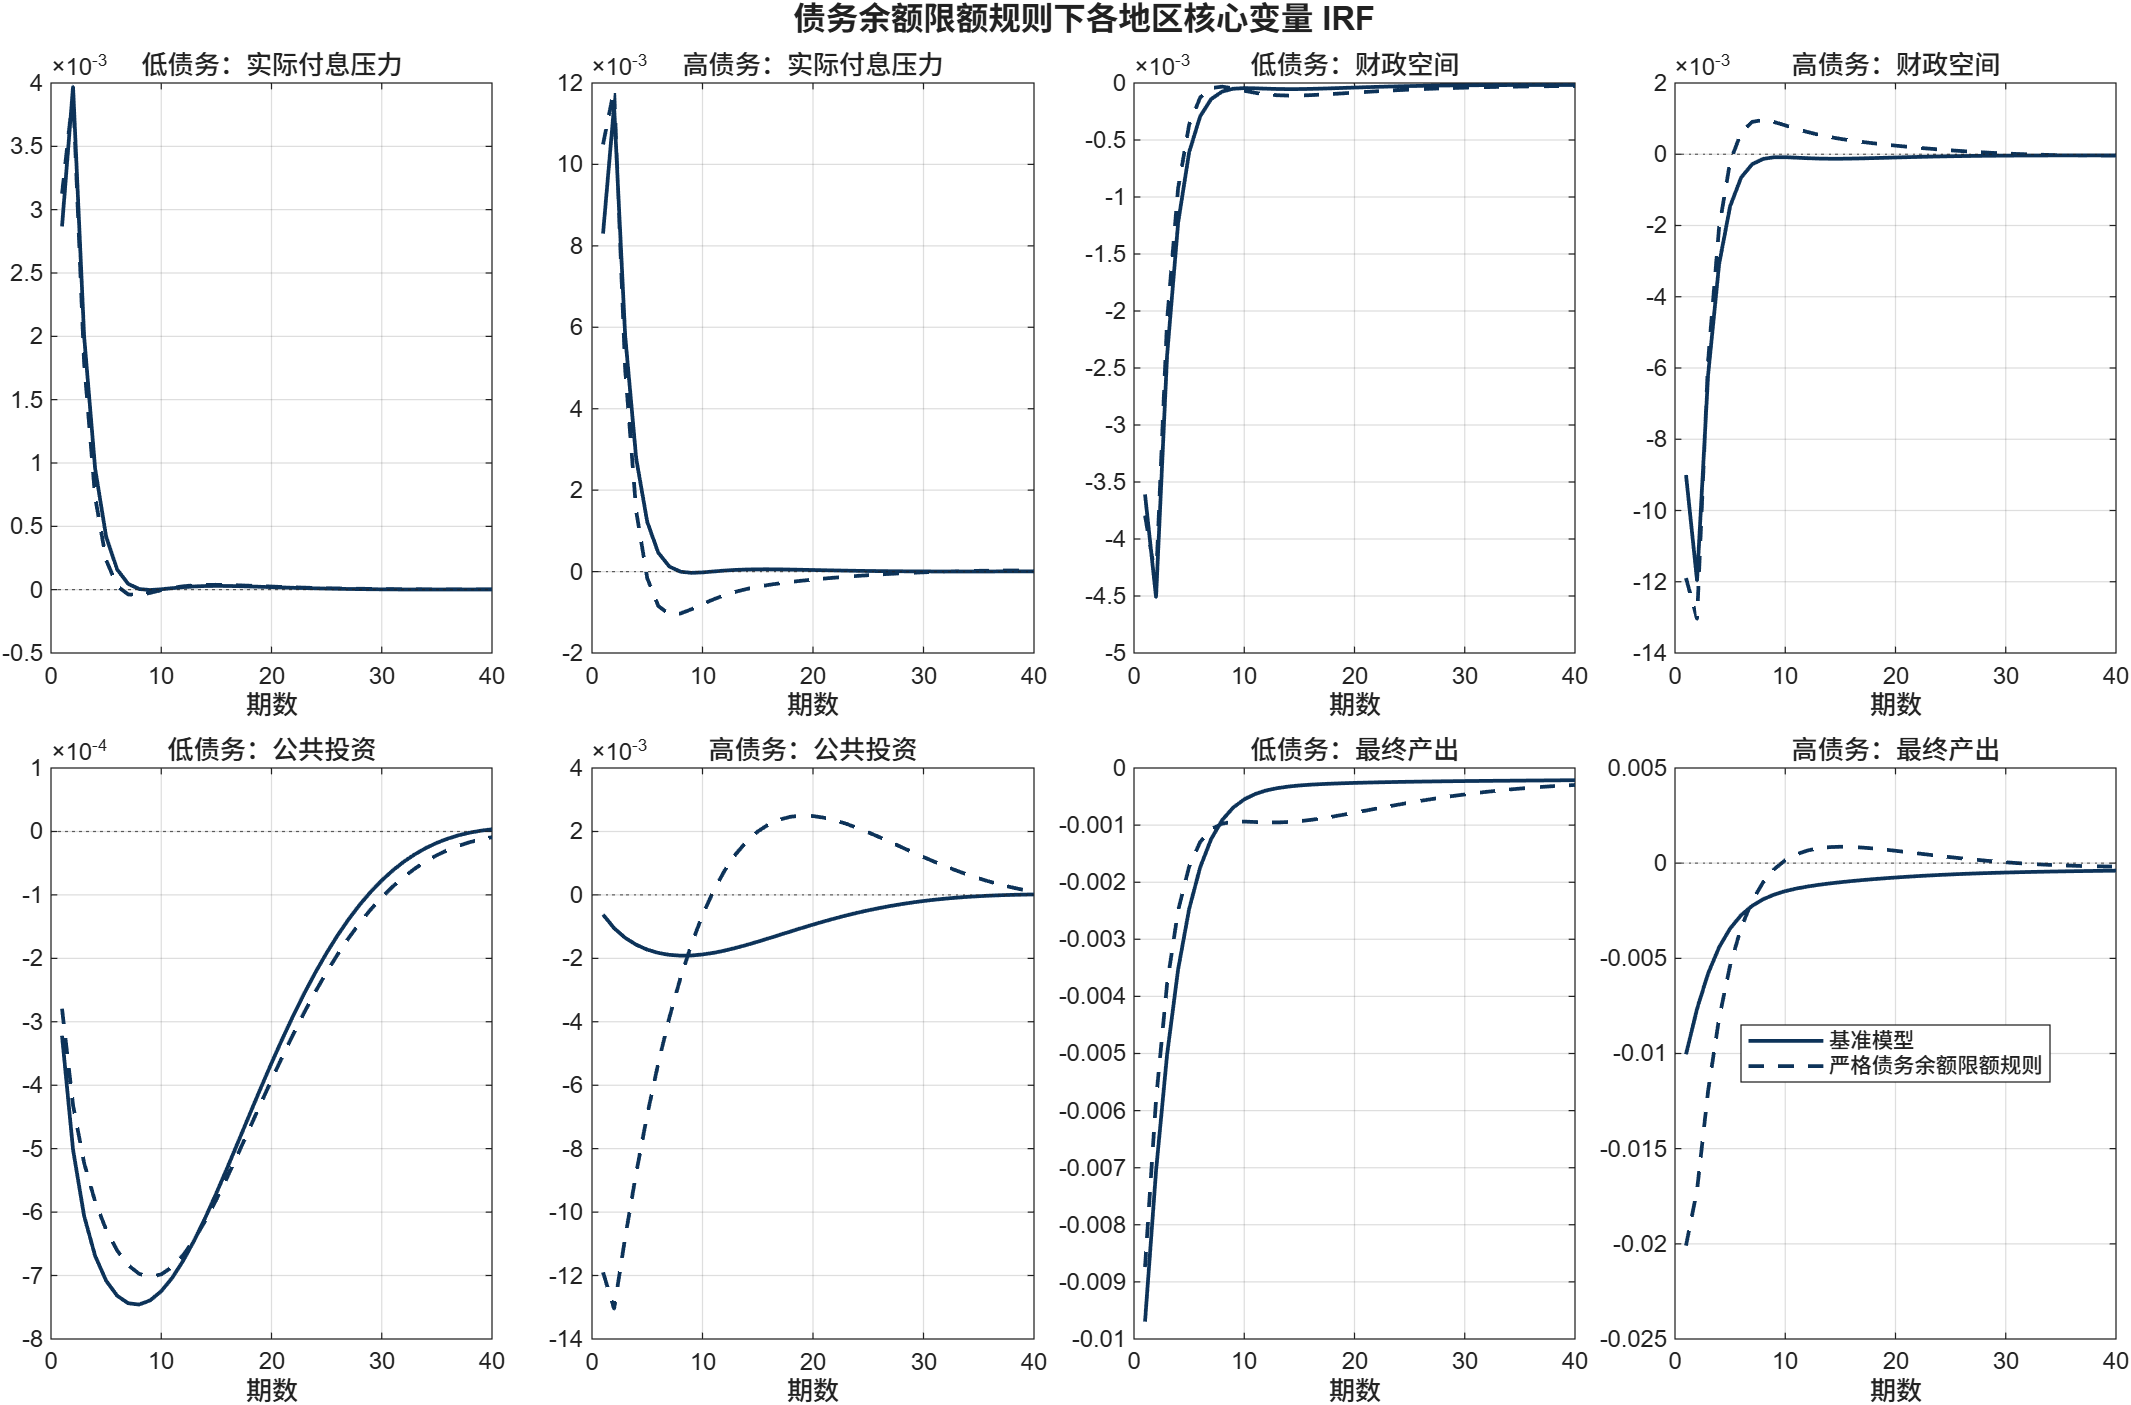
\includegraphics[width=0.92\textwidth]{code/policy_counterfactual/figure5_debt_limit_region_irfs.png}
		\caption{反事实政策实验：债务余额限额规则下各地区核心变量完整 IRF}
		\label{fig:app_debt_limit_regions}
	\end{figure}
	
	\subsection{经济规模与发展水平异质性稳健性检验}
	
	图 \ref{fig:app_scale_development} 展示了正文表 \ref{tab:scale_development_robustness} 所对应的完整动态轨迹。三组情景下高债务欠发达地区的政策利率、实际付息压力、财政空间、公共投资、公共资本、最终产出、消费与通胀响应高度贴合，说明区域规模权重变化并未改变地方债务--公共投资渠道的核心传导方向。
	
	\begin{figure}[H]
		\centering
		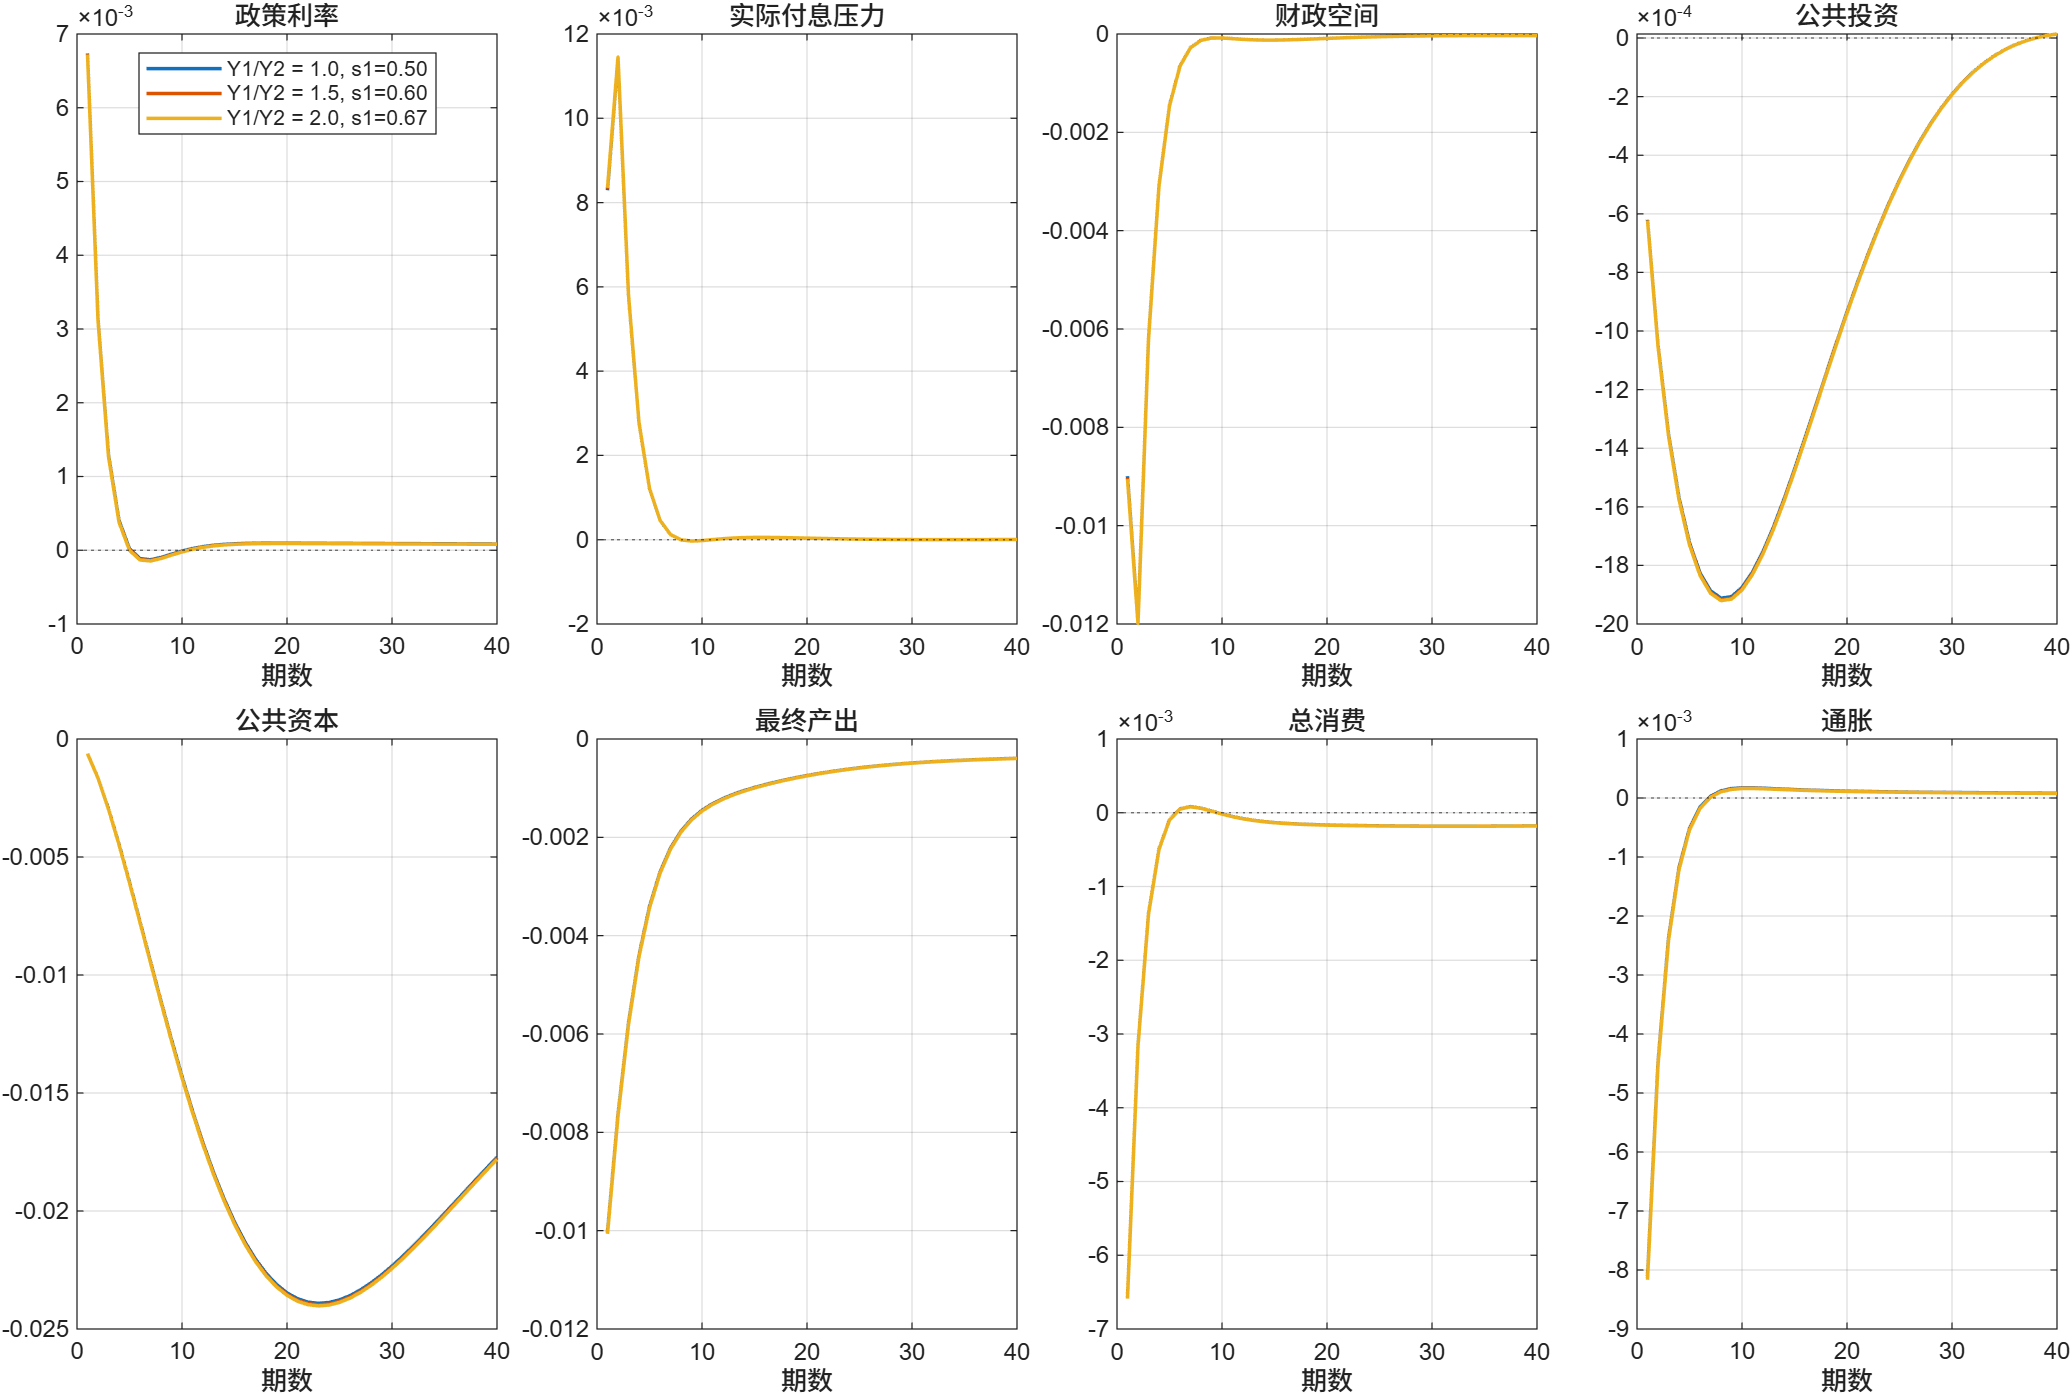
\includegraphics[width=0.90\textwidth]{code/scale_development/figure3_scale_development_region2_irfs.png}
		\caption{经济规模与发展水平异质性设定下的高债务地区完整脉冲响应}
		\label{fig:app_scale_development}
	\end{figure}
	
	\subsection{非对称扩展情景与跨地区投入产出网络密度检验}
	
	图 \ref{fig:app_extension_diff} 集中展示了当模型系统进一步激活地方债风险溢价内生化（$\mu_B>0$）、中央转移支付对地方赤字前瞻反应以及调节两地区最终品 CES 生产网络中的跨地区相互依赖弹性（更强或更弱的区域间投入产出联系密度）时，高低债务地区关键核心变量差异响应（Gap IRFs, 即地区 2 减地区 1）的演化轨迹。
	
	\begin{figure}[H]
		\centering
		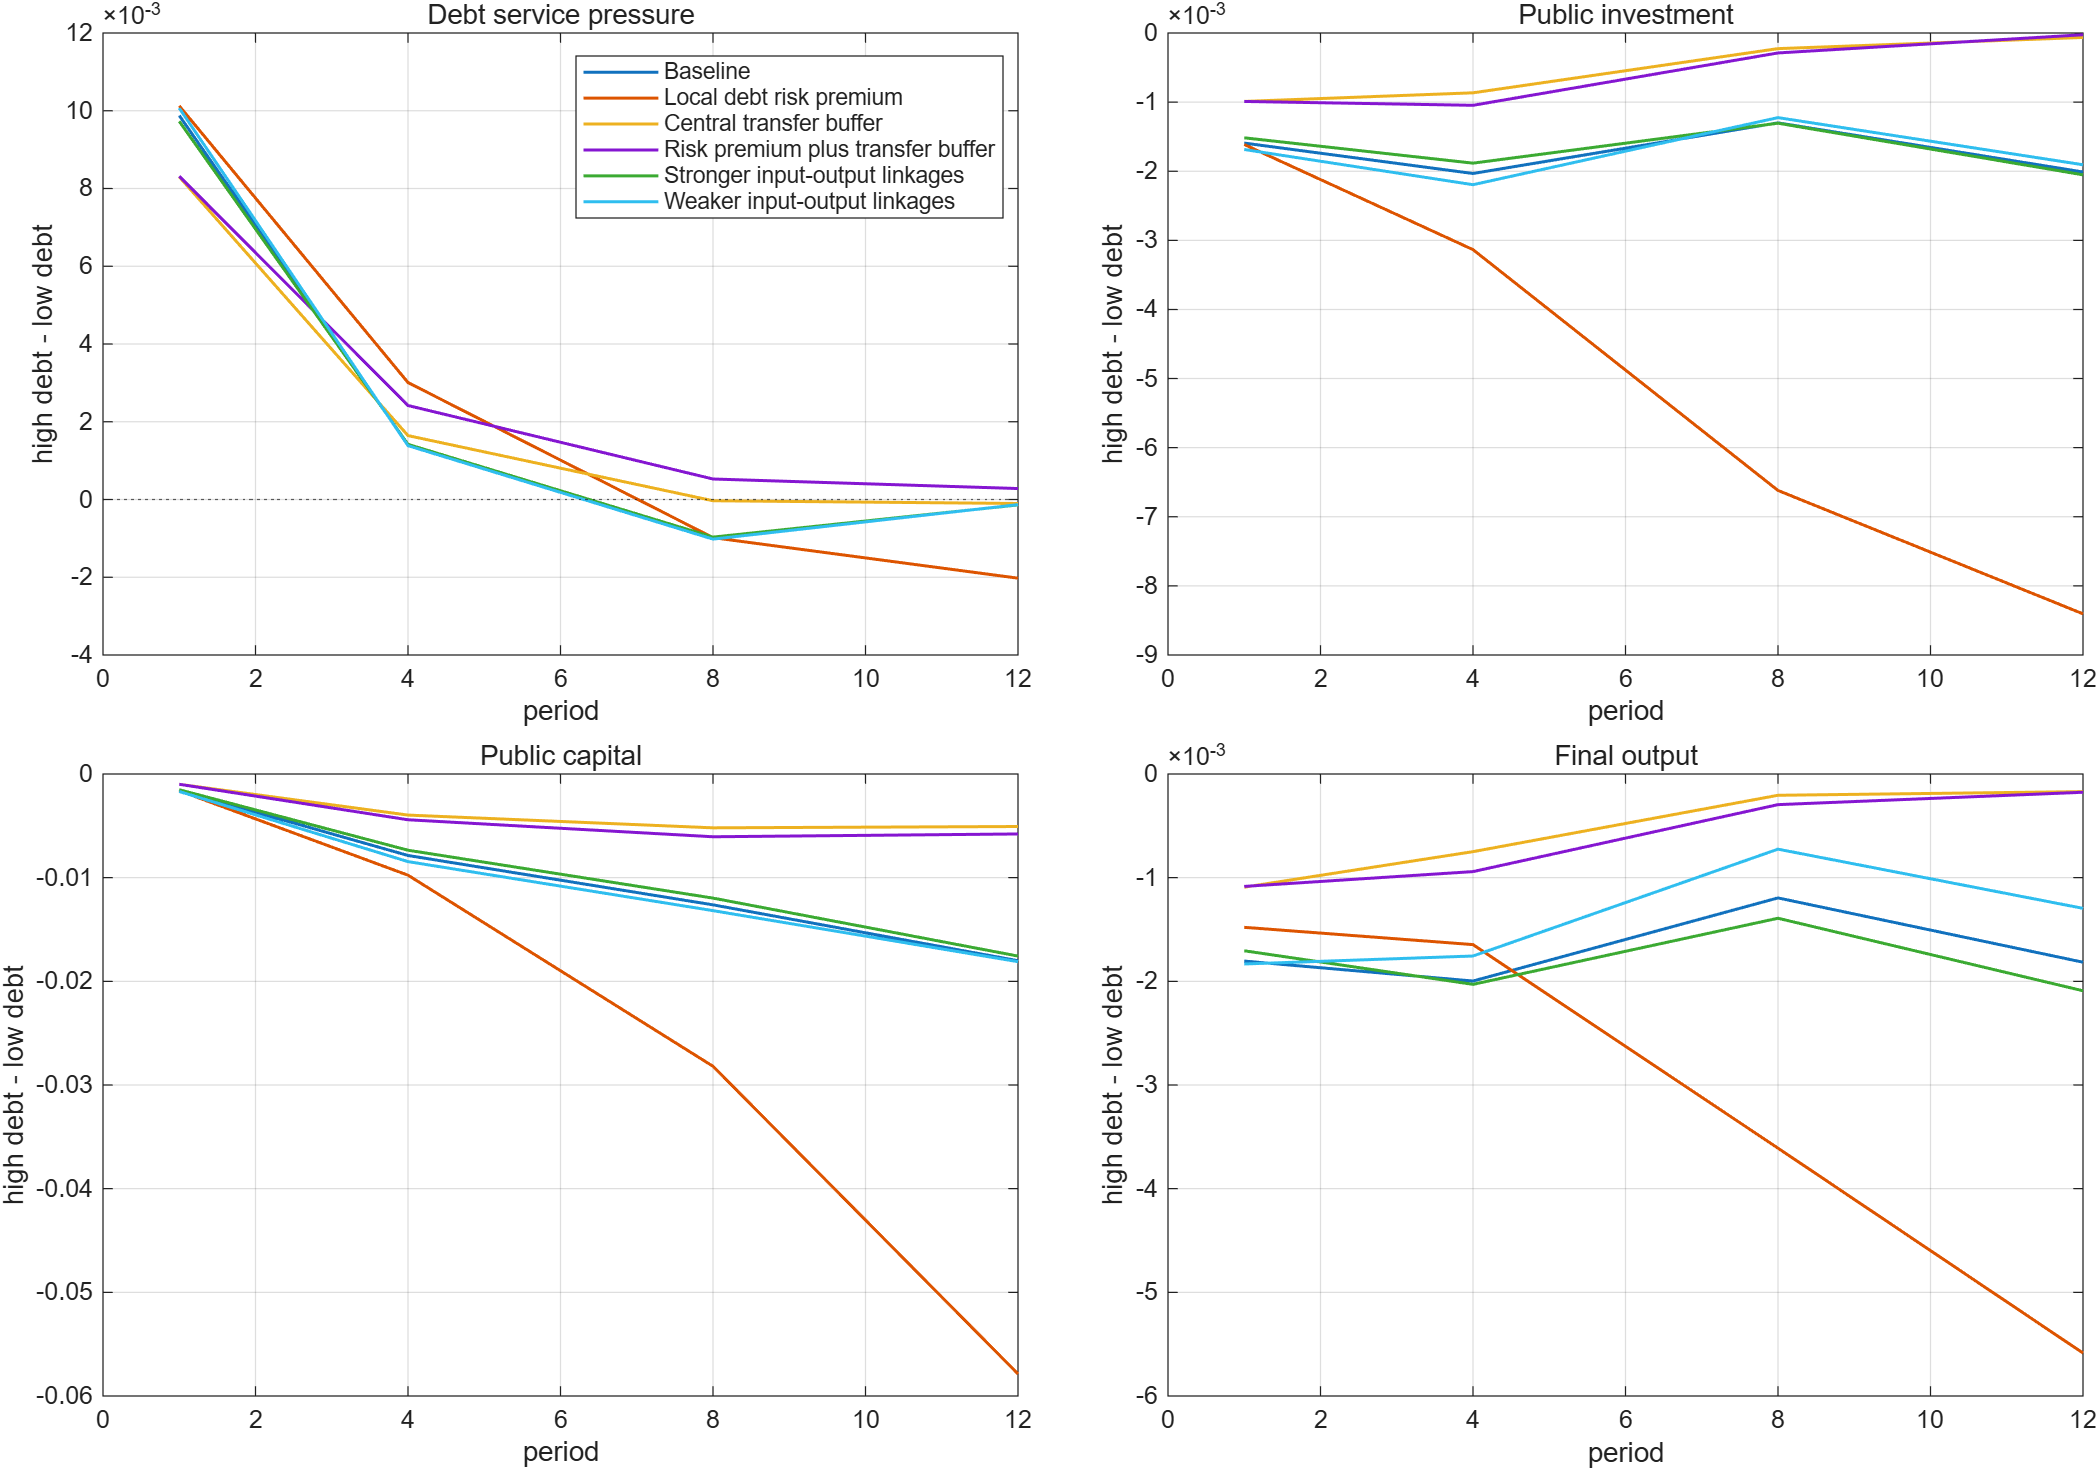
\includegraphics[width=0.90\textwidth]{code/extension_scenarios/extension_scenario_diff_irfs.png}
		\caption{多维扩展情景下高低债务地区关键核心变量差异响应脉冲对比}
		\label{fig:app_extension_diff}
	\end{figure}
	
	技术结果表明，当地方债利息溢价渠道被激活（即高债务地区面临更高的再融资边际风险惩罚）时，两地间的公共投资差距与总产出失衡缺口将呈现进一步跨期走宽趋势；而当跨地区投入产出网络密度增强（相对替代弹性 $\eta$ 下降）时，地区间的总需求外溢更强，高债务地区的生产放缓会通过供应链网络更大程度地影响低债务地区的最终产出，从而使得虽然两地实体层面的非对称不同步程度有所缓和，但付息压力的异质性负担依然存在。这说明本文核心渠道能够与供应链一般均衡网络机制相容。本附录所涉及的其余 6 类具体情景（包含纯粹风险溢价、强弱 IO 联系等）对应的独立绝对轨迹已完整保存在数值计算输出目录中，其结论与正文第四节的系统性评述一致。
	
	\subsection{探索性反事实：具有地区平衡特征的 Taylor 利率规则评估}
	
	图 \ref{fig:app_regional_balance_gap} 展示了一类探索性反事实场景：若中央银行在 Taylor 利率规则中显式纳入高债务地区相对于低债务地区的产出非对称分化项（式 \eqref{a41}，设定区域均衡目标参数 $\phi_{reg}=2.0$），系统核心变量差异的演化特征。该设定用于度量区域同步目标在模型中的边际稳定收益，并不表示现实中央银行应直接承担地方债务风险协调职能。
	
	\begin{figure}[H]
		\centering
		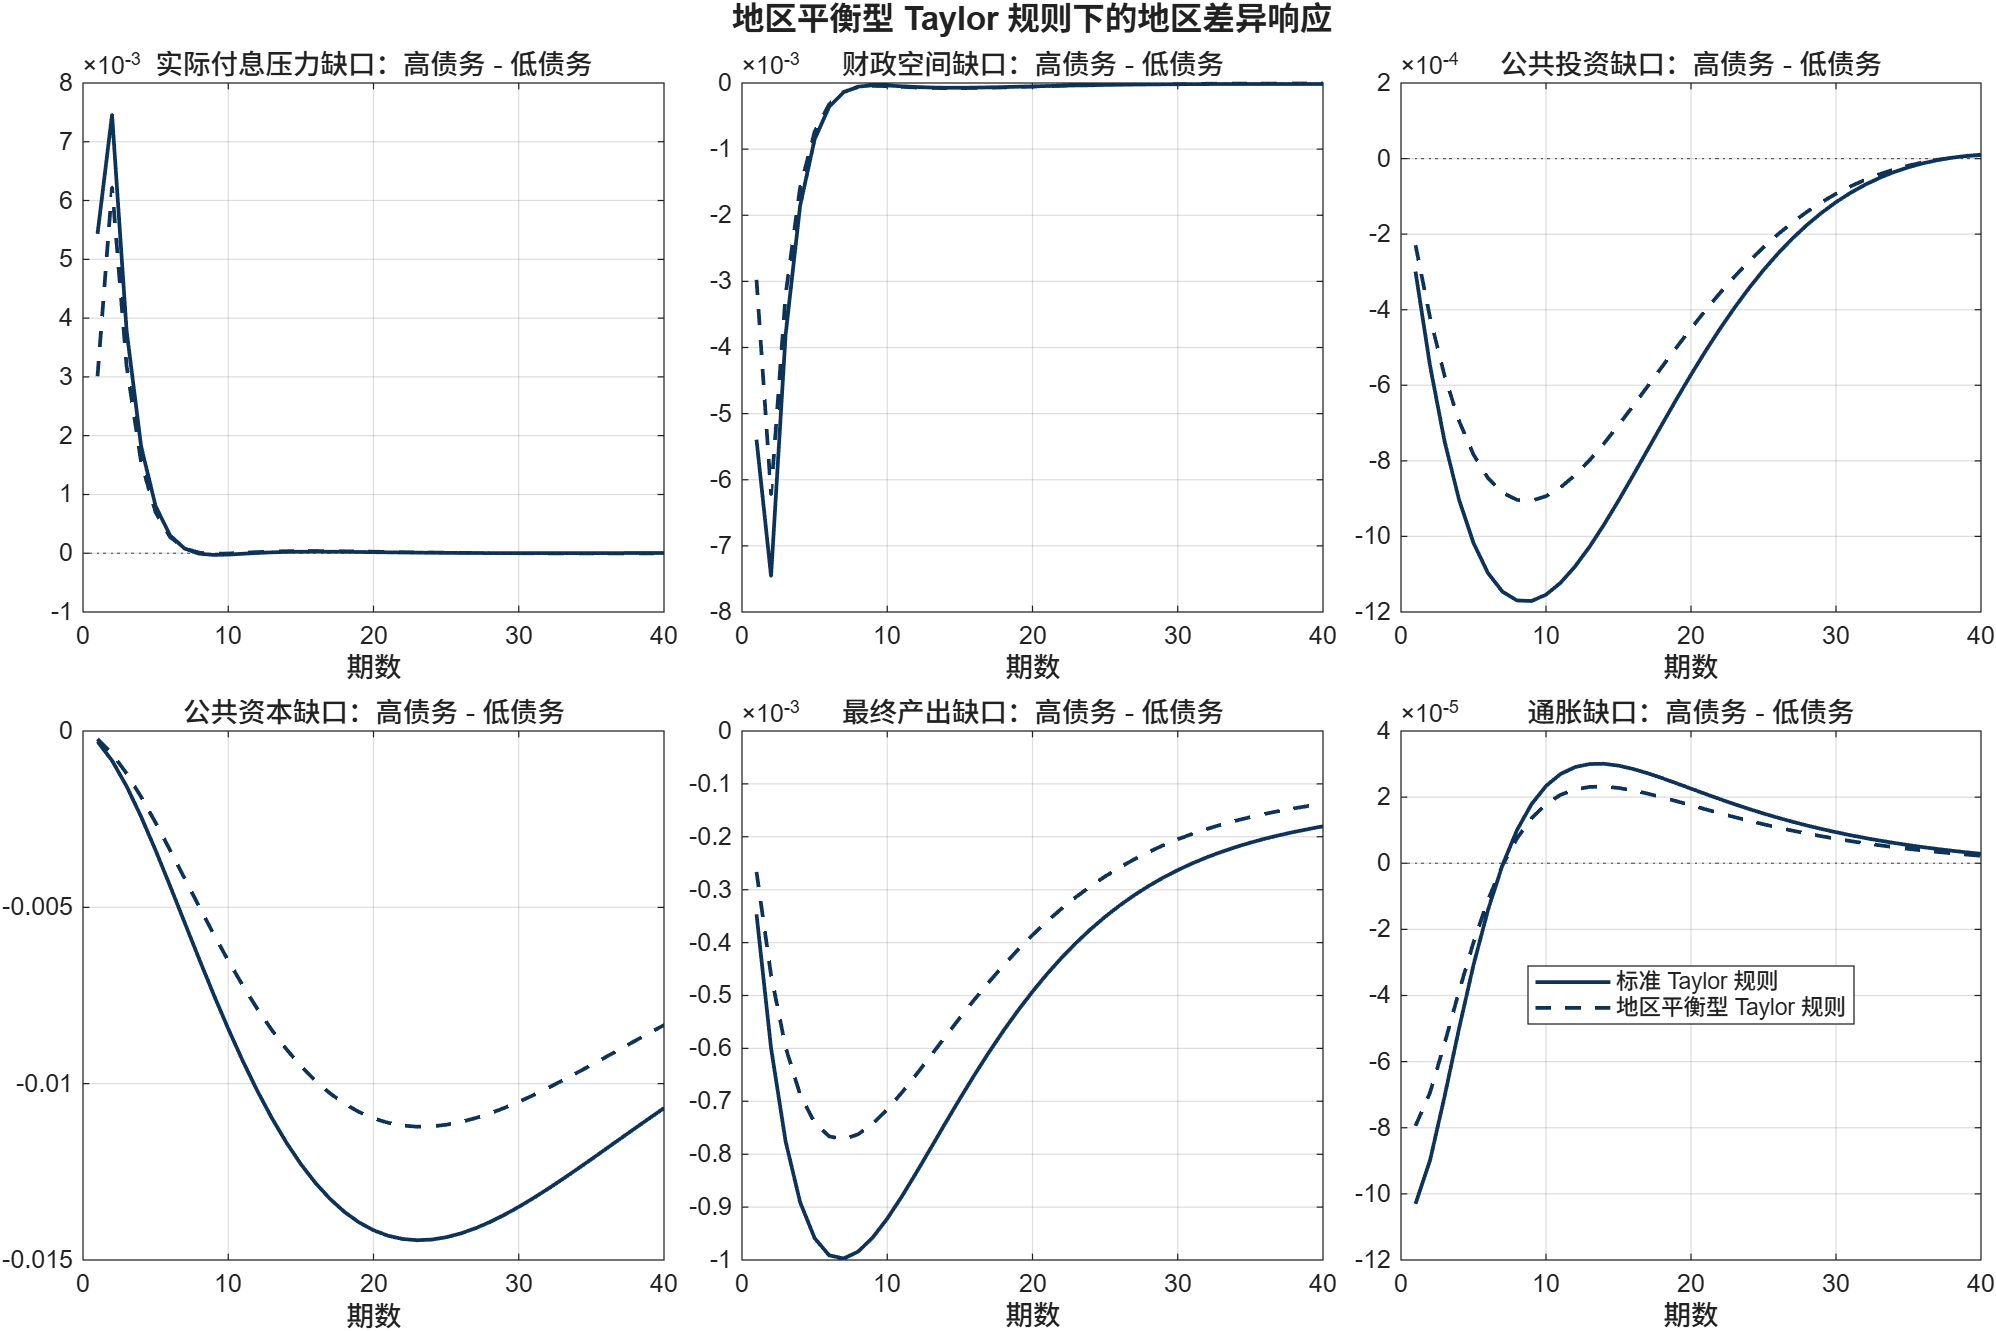
\includegraphics[width=0.90\textwidth]{code/policy_counterfactual/figure7_regional_balance_gap_irfs.png}
		\caption{探索性反事实：地区平衡型 Taylor 货币规则下的区域差异对冲成效}
		\label{fig:app_regional_balance_gap}
	\end{figure}
	
	定量轨迹表明：当统一中央银行在规则中考虑区域协调目标后，面对统一紧缩冲击，规则会对高债务地区的额外产出下行作出反应，从而推动无风险利率实施更有弹性的跨期调整。两地区产出缺口峰值由基准 Taylor 规则下的 $0.000997$ 降至 $0.000772$，公共投资缺口峰值由 $0.001171$ 降至 $0.000905$，地区间公共投资缺口与最终产出缺口更快向零轴收敛。这一探索性实验说明，区域同步性目标在模型中可能具有稳定收益，但其现实可行性取决于中央银行职责边界、区域产出缺口实时测度误差以及财政政策能否承担更直接的地区协调功能。
	
	\section{非线性动态方程组}
	
	本节列出与正文基准模型对应的非线性动态方程系统。与规则型公共投资版本不同，地方公共投资不再由简化式反应函数决定，而是由地方政府预算约束、公共资本积累约束、公共投资一阶条件、公共资本 Euler 方程和债务 Euler 方程共同内生决定。除货币政策创新和需求楔子外，基准系统不设置独立的技术、地方支出或转移支付随机冲击。
	
	\subsection{金融资产、TANK 居民行为与私人资本动态（对 \texorpdfstring{$j=1,2$}{j=1,2}）}
	\begin{align}
		\Lambda_{R,t}^1 &=(C_{R,t}^1)^{-\sigma} \label{a1}\\
		\Lambda_{R,t}^1 &=\beta E_t\left[\Lambda_{R,t+1}^1\frac{R_t}{\Pi_{t+1}^1}\right]\exp(-D_t) \label{a2}\\
		\Lambda_{R,t}^2 &=(C_{R,t}^2)^{-\sigma} \label{a3}\\
		\Lambda_{R,t}^2 &=\Lambda_{R,t}^1\frac{Q_{1,t}^1}{Q_{1,t}^2} \label{a4}\\
		\chi_N(N_{R,t}^j)^{\varphi} &=\Lambda_{R,t}^jW_t^j \label{a5}\\
		C_{H,t}^j &=W_t^jN_{H,t}^j+TR_{H,t}^j \label{a6}\\
		\chi_N(N_{H,t}^j)^{\varphi} &=(C_{H,t}^j)^{-\sigma}W_t^j \label{a7}\\
		C_t^j &=(1-\lambda_j)C_{R,t}^j+\lambda_jC_{H,t}^j \label{a8}\\
		N_t^j &=(1-\lambda_j)N_{R,t}^j+\lambda_jN_{H,t}^j \label{a9}\\
		K_{t+1}^j &=(1-\delta_K)K_t^j+ \left[1-\frac{\phi_I}{2}\left(\frac{I_t^j}{I_{t-1}^j}-1\right)^2\right]I_t^j \label{a10}\\
		Q_{K,t}^j
		&=\beta E_t\left[
		\frac{\Lambda_{R,t+1}^j}{\Lambda_{R,t}^j}
		\left(R_{K,t+1}^j+(1-\delta_K)Q_{K,t+1}^j\right)
		\right] \label{a11}\\
		1
		&=Q_{K,t}^j
		\left[
		1-\frac{\phi_I}{2}\left(\frac{I_t^j}{I_{t-1}^j}-1\right)^2
		-\phi_I\left(\frac{I_t^j}{I_{t-1}^j}-1\right)\frac{I_t^j}{I_{t-1}^j}
		\right] \notag\\
		&\quad+\beta E_t\left[
		\frac{\Lambda_{R,t+1}^j}{\Lambda_{R,t}^j}
		Q_{K,t+1}^j
		\phi_I\left(\frac{I_{t+1}^j}{I_t^j}-1\right)
		\left(\frac{I_{t+1}^j}{I_t^j}\right)^2
		\right] \label{a12}
	\end{align}
	
	\subsection{最终品 CES 制造与跨区域相对价格动态（对 \texorpdfstring{$j=1,2$}{j=1,2}）}
	\begin{align}
		1 &=\left[ \omega_j(Q_{j,t}^j)^{1-\eta} +(1-\omega_j)(Q_{-j,t}^j)^{1-\eta} \right]^{\frac{1}{1-\eta}} \label{a13}\\
		M_{j,t}^j &=\omega_j(Q_{j,t}^j)^{-\eta}Y_t^j \label{a14}\\
		M_{-j,t}^j &=(1-\omega_j)(Q_{-j,t}^j)^{-\eta}Y_t^j \label{a15}
	\end{align}
	对于全部四种区域交互组合（对所有 $k \in \{1,2\}$ 与 $j \in \{1,2\}$），其计价相对价格跨期闭合满足：
	\begin{equation}
		\frac{Q_{k,t}^j}{Q_{k,t-1}^j}=\frac{\Pi_{M,t}^k}{\Pi_t^j} \label{a16}
	\end{equation}
	
	\subsection{中间品供给网络、要素分成与 Calvo 定价辅助递归（对 \texorpdfstring{$j=1,2$}{j=1,2}）}
	\begin{align}
		A_t^j &=1 \label{a17}\\
		Y_{M,t}^j &=\frac{A_t^j(K_{G,t}^j)^{\gamma_G}(K_t^j)^{\alpha}(N_t^j)^{1-\alpha}}{V_t^j} \label{a18}\\
		W_t^j &=(1-\alpha)Q_{j,t}^jMC_t^j\frac{Y_{M,t}^jV_t^j}{N_t^j} \label{a19}\\
		R_{K,t}^j &=\alpha Q_{j,t}^jMC_t^j\frac{Y_{M,t}^jV_t^j}{K_t^j} \label{a20}\\
		Y_{M,t}^j &=M_{j,t}^1+M_{j,t}^2 \label{a21}\\
		1 &=(1-\theta_p)(p_{*,t}^j)^{1-\epsilon_p}+\theta_p(\Pi_{M,t}^j)^{\epsilon_p-1} \label{a22}\\
		X_{1,t}^j &=\Lambda_{R,t}^jQ_{j,t}^jMC_t^jY_{M,t}^j +\beta\theta_pE_t\left[(\Pi_{M,t+1}^j)^{\epsilon_p}X_{1,t+1}^j\right] \label{a23}\\
		X_{2,t}^j &=\Lambda_{R,t}^jQ_{j,t}^jY_{M,t}^j +\beta\theta_pE_t\left[(\Pi_{M,t+1}^j)^{\epsilon_p-1}X_{2,t+1}^j\right] \label{a24}\\
		p_{*,t}^j &=\frac{\epsilon_p}{\epsilon_p-1}\frac{X_{1,t}^j}{X_{2,t}^j} \label{a25}\\
		V_t^j &=(1-\theta_p)(p_{*,t}^j)^{-\epsilon_p}+\theta_p(\Pi_{M,t}^j)^{\epsilon_p}V_{t-1}^j \label{a26}
	\end{align}
	
	
	
\subsection{地方国库、内生公共资本与地方政府最优选择系统（对 \texorpdfstring{$j=1,2$}{j=1,2}）}

为便于核对地方政府最优条件，本小节同时保留预算约束、公共资本积累方程和两条 Euler 方程。式 \eqref{a34} 左侧括号中的三项分别来自新增一单位公共投资的直接预算成本、当期公共投资调整成本的一阶导数以及调整成本随投资规模变化形成的附加边际项；右侧的前瞻项来自 $I_{G,t}^j$ 作为下一期调整成本分母时对未来预算成本的影响。式 \eqref{a37} 左侧为新增债务带来的当期可用财政资源，并扣除债务管理成本的边际占用；右侧为下一期实际偿还成本，其中括号内的 $\mu_B$ 项来自地方债利率对当期债务率的边际反应。正文基准取 $\mu_B=0$ 时，该风险溢价边际项退化为 1。
\begin{align}
	DS_t^j
	&=\left(\frac{R_{B,t-1}^j}{\Pi_t^j}-1\right)\frac{B_{t-1}^j}{Y_t^j}, \label{a27}\\
	FS_t^j
	&=(1-\theta_T)\tau_Y Y_t^j+Z_t^j
	-\left(\frac{R_{B,t-1}^j}{\Pi_t^j}-1\right)B_{t-1}^j
	-G_t^j-\lambda_jTR_{H,t}^j, \label{a28}\\
	\Phi_{I,t}^j
	&=\frac{\chi_I}{2}
	\left(\frac{I_{G,t}^j}{I_{G,t-1}^j}-1\right)^2 I_{G,t}^j, \label{a29}\\
	\Phi_{B,t}^j
	&=\frac{\varphi_B}{2}
	\left(\frac{B_t^j}{\bar Y^j}-\bar b^j\right)^2\bar Y^j, \label{a30}\\
	\frac{R_{B,t}^j}{R_t}
	&=\exp\left[
	\mu_B\left(
	\frac{B_t^j/Y_t^j}{\bar B^j/\bar Y^j}-1
	\right)
	\right], \label{a31}\\
	B_t^j
	&=\frac{R_{B,t-1}^j}{\Pi_t^j}B_{t-1}^j
	+G_t^j+I_{G,t}^j+\Phi_{I,t}^j+\Phi_{B,t}^j+\lambda_jTR_{H,t}^j
	-(1-\theta_T)\tau_Y Y_t^j-Z_t^j, \label{a32}\\
	K_{G,t+1}^j
	&=(1-\delta_G)K_{G,t}^j+I_{G,t}^j, \label{a33}\\
	\Lambda_{G,t}^j
	&\left[
	1+\chi_I\left(\frac{I_{G,t}^j}{I_{G,t-1}^j}-1\right)
	\frac{I_{G,t}^j}{I_{G,t-1}^j}
	+\frac{\chi_I}{2}
	\left(\frac{I_{G,t}^j}{I_{G,t-1}^j}-1\right)^2
	\right] \notag\\
	&=Q_{G,t}^j
	+\beta_G E_t\left[
	\Lambda_{G,t+1}^j\chi_I
	\left(\frac{I_{G,t+1}^j}{I_{G,t}^j}-1\right)
	\left(\frac{I_{G,t+1}^j}{I_{G,t}^j}\right)^2
	\right], \label{a34}\\
	Q_{G,t}^j
	&=\beta_G E_t\left[
	MB_{G,t+1}^j+(1-\delta_G)Q_{G,t+1}^j
	\right], \label{a35}\\
	MB_{G,t}^j
	&=\omega_Y\frac{\gamma_G}{K_{G,t}^j}
	+\Lambda_{G,t}^j(1-\theta_T)\tau_Y\gamma_G\frac{Y_t^j}{K_{G,t}^j}, \label{a36}\\
	\Lambda_{G,t}^j
	&\left[
	1-\varphi_B\left(\frac{B_t^j}{\bar Y^j}-\bar b^j\right)
	\right] \notag\\
	&=\beta_G E_t\left[
	\Lambda_{G,t+1}^j
	\frac{R_{B,t}^j}{\Pi_{t+1}^j}
	\left(
	1+\mu_B\frac{B_t^j/Y_t^j}{\bar B^j/\bar Y^j}
	\right)
	\right], \label{a37}\\
	\log\left(\frac{G_t^j}{\bar G^j}\right)
	&=\rho_G\log\left(\frac{G_{t-1}^j}{\bar G^j}\right), \label{a38}\\
	\log\left(\frac{TR_{H,t}^j}{\bar{TR}_H^j}\right)
	&=\rho_{TR}\log\left(\frac{TR_{H,t-1}^j}{\bar{TR}_H^j}\right), \label{a39}\\
	\log\left(\frac{Z_t^j}{\bar Z^j}\right)
	&=\rho_Z\log\left(\frac{Z_{t-1}^j}{\bar Z^j}\right)
	+\phi_{Z,DS}\left(\frac{DS_t^j}{\bar{DS}^j}-1\right) \notag\\
	&\quad
	+\phi_{Z,B}
	\left(
	\frac{B_{t-1}^j/Y_{t-1}^j}{\bar B^j/\bar Y^j}-1
	\right). \label{a40z}
\end{align}
	
\subsection{总体加权模块、Taylor 货币政策与总体市场资源出清}
	\begin{align}
		Y_t &=s_1Y_t^1+s_2Y_t^2 \label{a39y}\\
		\Pi_t &=(\Pi_t^1)^{s_1}(\Pi_t^2)^{s_2} \label{a39pi}\\
		MP_t &=\rho_{MP}MP_{t-1}+\varepsilon_{MP,t} \label{a39mp}\\
		D_t &=\rho_D D_{t-1} - \varepsilon_{D,t} \label{a41D}\\
		\frac{R_t}{\bar R}
		&=\left(\frac{R_{t-1}}{\bar R}\right)^{\rho_R}
		\left[
		\left(\frac{\Pi_t}{\bar\Pi}\right)^{\phi_\pi}
		\left(\frac{Y_t}{\bar Y}\right)^{\phi_Y}
		\right]^{1-\rho_R}
		\exp(MP_t) \label{a41}
	\end{align}
	最终品总体出清资源约束对 $j=1,2$：
	\begin{equation}
		Y_t^j=C_t^j+I_t^j+G_t^j+I_{G,t}^j+\Phi_{I,t}^j+\Phi_{B,t}^j \label{a42}
	\end{equation}
	
\end{document}
